\documentclass[11pt]{book}
\usepackage{fontspec}
\setmainfont{TeX Gyre Pagella}
\usepackage{amsmath,amssymb,amsthm}
\usepackage[margin=1.3in]{geometry}
\usepackage{titlesec}
\usepackage{graphicx}
\usepackage{caption}
\usepackage{needspace}
\usepackage{tikz}
\usetikzlibrary{arrows.meta,positioning,calc,fit,backgrounds,shapes.geometric,decorations.pathreplacing}

\newtheorem{theorem}{Theorem}[chapter]
\newtheorem{definition}[theorem]{Definition}
\newtheorem{lemma}[theorem]{Lemma}
\newtheorem{proposition}[theorem]{Proposition}
\newtheorem{corollary}[theorem]{Corollary}
\newtheorem{remark}[theorem]{Remark}
\newtheorem{example}[theorem]{Example}

\newtheorem*{appendixdefinition}{Definition}
\newtheorem*{appendixlemma}{Lemma}
\newtheorem*{appendixproposition}{Proposition}
\newtheorem*{appendixtheorem}{Theorem}
\newtheorem*{appendixcorollary}{Corollary}
\newtheorem*{appendixremark}{Remark}
\newtheorem*{appendixexample}{Example}

\title{Mathematical Proof for the Existence of God\\[0.3em]\large A Study in Constraint Theology}
\author{Flyxion\\Independent Researcher}
\date{}

\begin{document}

\newgeometry{margin=0pt}
\thispagestyle{empty}
\noindent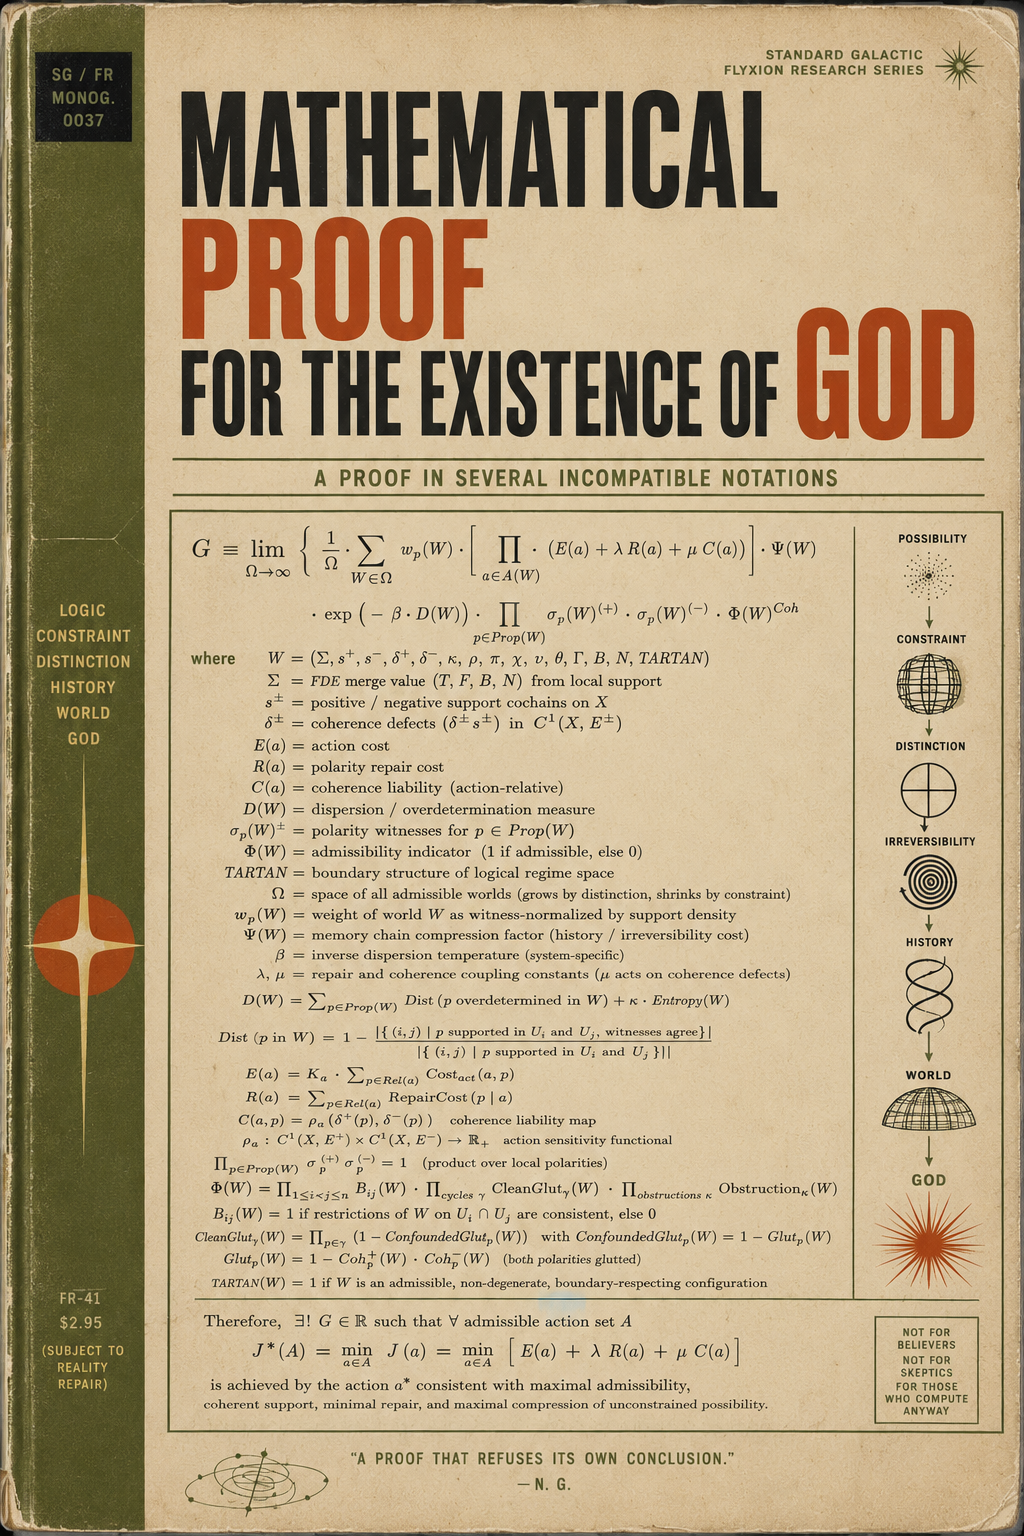
\includegraphics[width=\paperwidth,height=\paperheight]{figures/cover.png}
\clearpage
\restoregeometry

\maketitle

\chapter*{Author's Note}
\addcontentsline{toc}{chapter}{Author's Note}

Everything from the Preface onward is written in character, as a straight-faced mathematical monograph, deliberately without the usual signposting that would keep reminding the reader it's a joke. This short note is not part of that voice. It's me.

This book belongs to the tradition of \emph{A Modest Proposal}: an argument built with complete formal seriousness toward a conclusion no reasonable person is meant to accept literally, with real, checkable mathematics standing in for Swift's economics. I wrote it as a hobby, in spare time around a manual, physical day job, on an ordinary sleep schedule. It is not a claim to have discovered anything about the universe, and the book itself says so explicitly and repeatedly, at some length, starting in Chapter 1 and not letting up until the very last appendix. If you take away one sentence from this note, take this one: nowhere in the four hundred-odd pages that follow does anyone, including me, believe that a formal object satisfying some definitions is the same thing as a god.

I'd rather you check the proofs than take my word for any of this, including this note. That's rather the point.

\bigskip
\begin{center}
\begin{minipage}{0.75\textwidth}
\itshape
He promised to make them a beautiful philosophical book, written very small for their usage, and said that in this book they would see the point of everything. Indeed, he gave them this book before leaving. It was taken to the academy of science in Paris, but when the ancient secretary opened it, he saw nothing but blank pages.

``Ah!'' he said, ``I suspected as much.''
\end{minipage}

\medskip
\upshape
--- Voltaire, \emph{Micromégas} (1752), trans. Peter Phalen
\end{center}
\bigskip

\chapter*{Preface}
\addcontentsline{toc}{chapter}{Preface}

This is a work of mathematics. It contains definitions, lemmas, theorems, and a proof. It also contains a title that most readers will find provocative, and a small number of readers will find offensive, and an even smaller number will find, upon finishing the book, to have been earned. All three reactions are correct.

The book proves exactly what it proves, and nothing more. This sentence will be repeated, in various forms, throughout the text, because it is the single claim the author is least willing to have misquoted. A formal object is constructed. Properties of that object are derived. Near the end, a name is proposed for the object. The proposal is then examined with the same rigor applied to everything preceding it, and found to be under-determined by the mathematics that produced it.

Readers hoping for a disproof of atheism, or a disproof of theism, or an argument for any particular religious tradition, will not find one here. Readers hoping for a rigorous account of what a constraint system can and cannot license us to say about ultimate explanation will find quite a lot.

The book is organized so that the word ``God'' does not appear in a load-bearing capacity until Part V. Everything before that point is ordinary, checkable mathematics, and should be read as such. Everything after that point is philosophy, and should be read as such. The distinction between derivation and interpretation will occupy the remainder of this book.

\chapter*{A Disclaimer That Will Not Be Read}
\addcontentsline{toc}{chapter}{A Disclaimer That Will Not Be Read}

No theorem in this book asserts the existence of a personal deity, a conscious agent, an intentional creator, or an object appropriate for worship. Every theorem in this book asserts the existence, uniqueness, or structural properties of a mathematical object defined by the author. Readers who confuse the two categories are invited to reread Chapter 24, at which point the confusion becomes the subject rather than an accident.

\part{The Problem Before the Proof}

\chapter*{A Note on Origins}
\addcontentsline{toc}{chapter}{A Note on Origins}

Nothing in the construction that follows is new in the sense of having no antecedent. What may be new, if anything is, is the particular combination, and the insistence on carrying it through to a single terminal definition rather than leaving each piece to do its usual, separate work. It is worth naming the antecedents before the construction begins, so that no reader mistakes synthesis for invention.

The question of how something persists as itself through change is at least as old as Aristotle's discussion of substance and accident, and reappears, transformed, wherever a discipline needs to say what stays fixed while something else varies. Leibniz's identity of indiscernibles, the principle that two things sharing every property are one thing, is the ancestor of this book's quotient construction (Chapter 6): a distinction space does not merely tolerate indistinguishable elements, it identifies them, and this was Leibniz's proposal about identity in general, applied here to a deliberately minimal notion of distinguishability rather than to the full richness of properties he had in mind.

Error-correcting codes, developed by Hamming and Shannon's immediate successors to let a message survive noise, are the ancestor of this book's repair apparatus (Chapters 9 and 13). A code does not prevent corruption; it makes corruption recoverable up to some bound, exactly the distinction this book draws between a state's being admissible and its being merely repairable. The repair cost of Definition 9.2 is, structurally, a distance-to-codeword computation dressed in more general clothing.

Sheaf theory, in the tradition running from Leray through Grothendieck, is the ancestor of this book's treatment of worlds as local data that may or may not glue to a global object (Chapter 11). The overlap condition of Proposition 11.6, and the failure mode of Proposition 11.4, are the same gluing condition sheaf theory has studied for the better part of a century, specialized here to admissibility data rather than to sections of a sheaf in the technical sense; this book does not develop sheaf-theoretic machinery in general and claims no result belonging to that literature.

Paraconsistent logic, associated with da Costa and developed extensively by Graham Priest, is the ancestor of this book's insistence that a contradiction need not be an error (Chapter 19). Priest's dialetheism, the view that some contradictions are true, is a stronger philosophical claim than this book makes; what this book borrows is the technical apparatus, first-degree entailment and the refusal of explosion, without committing to the view that the resulting gluts describe reality rather than merely a well-behaved formal system.

Information geometry, in the tradition associated with Amari, treats spaces of probability distributions as geometric objects in their own right, with their own notion of distance. This book's use of the Jensen--Shannon divergence to extend a distinction metric from points to distributions (Definition 8.5) is a small, specific instance of that same move, borrowed rather than developed.

None of these fields is being claimed as a hidden unity, and none of them would recognize this book as a contribution to their own literature. What they share, and what this book tries to make into a single object of study rather than five separate ones, is a recurring question: given that something can be lost, disturbed, or brought into disagreement with itself, under what conditions can it be told apart from its surroundings, kept, repaired, and continued. That question, asked once and answered by a single formalism rather than five, is this book's actual claim to originality, modest as that claim is.

\begin{appendixremark}
One further antecedent belongs here, offered more playfully than the rest and weighted accordingly. The Hebrew word for the serpent of Genesis 3, \emph{nachash}, shares its root with the verb meaning to hiss, to whisper, and, in several other biblical occurrences, to practice divination or enchantment; lexicographers going back to Gesenius have connected the noun to the sound of the hiss and the verb to the whispered incantations of a soothsayer, though the exact direction of derivation is debated. On that reading, the serpent's opening move, ``did God really say,'' is not primarily a lie but a whispered reinterpretation, an offered gloss on an instruction that was not, on its own terms, ambiguous. It is difficult, having spent this many chapters on Definition 2.2, not to notice that this is the shape of an interpretive leap, offered to the first available reader, about the meaning of the very first prohibition on record. Separately, and on somewhat firmer philological ground, the phrase usually rendered ``the knowledge of good and evil,'' \emph{hada'at tov vara}, uses two words, \emph{tov} and \emph{ra}, whose semantic range in Biblical Hebrew is broader than the English gloss suggests: \emph{tov} covers pleasing, fitting, and functioning as intended, and \emph{ra} covers harmful, ruinous, and broken, in addition to their more familiar moral senses. Read this way, the tree offers the knowledge of \emph{distinguishing what is pleasing from what is broken}, which is to say, on this book's own vocabulary, simply the capacity for distinction (Chapter 6) applied for the first time to a world that, until that verse, had none. A third point, briefer than the other two, sits one verse later. The pitch sealing the ark, \emph{kopher} (Genesis 6:14), comes from a root meaning simply to cover, the same root behind Arabic's ordinary word for a non-believer, \emph{kafir}: one who covers, or conceals, the truth. The wood the ark is built from, \emph{gopher}, named in the same verse, is a separate and unrelated word of uncertain origin, close enough in sound to its neighbor to invite confusion between them, and not merely by coincidence: $g$ and $k$ share a place of articulation, differing only in voicing, and Semitic consonants show exactly this alternation elsewhere. The letter \emph{gimel} gave Greek both \emph{gamma}, keeping the $g$, and, by way of the same root's word for camel, \emph{kamelos}, shifting to $k$, the direct ancestor of the English word. This book has had a great deal to say, since Chapter 2, about arguments that cover a gap in derivation rather than close it; a reader who wants to follow that resonance further is welcome to. This book takes no position on whether any of these readings is the correct one, only that it did not expect to find its own opening move waiting in Genesis 3, and thought a reader who has come this far deserved to be told.
\end{appendixremark}

\chapter{Every Proof Begins with a Definition}

A mathematical proof establishes that a conclusion follows from a set of premises by a sequence of licensed inferential steps. It does not establish that the premises are true of the world, that the conclusion is important, or that the symbols used in stating it mean what a reader outside the proof might assume them to mean. These are three separate questions, and a proof by itself answers none of them.

This distinction is not a technicality. It is the entire content of every dispute that has ever occurred between a mathematician who has proved something and a reader who feels that nothing has been shown. The mathematician is usually right about the derivation. The reader is usually right that the derivation does not settle what they wanted settled. Both parties are talking about the same symbols and about different things.

\begin{definition}
A \emph{formal system} is a triple $(L, A, R)$ consisting of a language $L$, a set of axioms $A \subseteq L$, and a set of inference rules $R$. A \emph{theorem} of the system is any sentence reachable from $A$ by finitely many applications of $R$.
\end{definition}

\begin{definition}
An \emph{interpretation} of a formal system is a function assigning elements of some domain $D$, together with relations and operations on $D$, to the non-logical symbols of $L$, such that the axioms of $A$ come out true under the assignment.
\end{definition}

Nothing in Definition 1.1 makes reference to interpretation. A formal system generates theorems whether or not anyone has ever proposed a domain for it to describe. This is what makes formal systems portable: the same axioms of group theory hold of rotations, of permutations, of residues modulo a prime, and of countless structures no one has yet thought to construct. It is also what makes formal systems dangerous when handled carelessly, because a reader presented with a theorem and a suggestive name for one of its symbols will supply an interpretation whether the author intends one or not.

The distinction between formal derivation and semantic interpretation will remain explicit throughout what follows.

\begin{remark}
Every ontological argument in the history of the subject can be read as a dispute, disguised as a proof, about whether a particular interpretation is forced by a particular formal system. None of them are proofs in the sense of Definition 1.1 unless the interpretive step is itself licensed by an inference rule, and in every case examined in Chapter 2, it is not.
\end{remark}

\begin{figure}[htb]
\centering
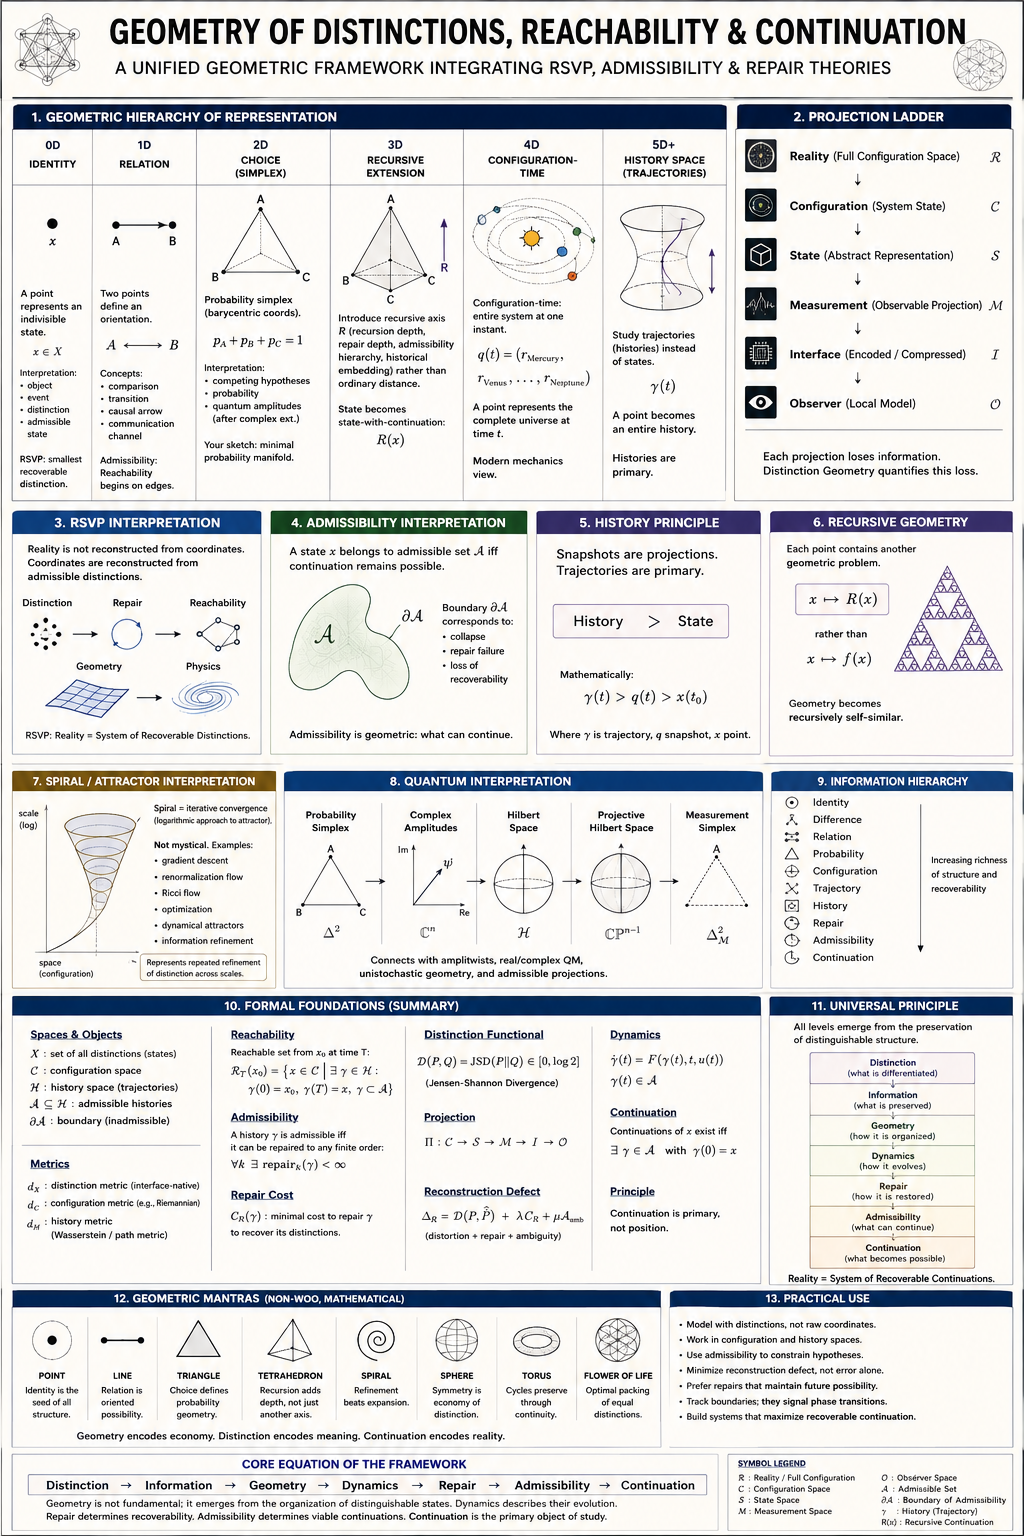
\includegraphics[width=\textwidth]{figures/dependency-diagram.png}
\captionsetup{width=0.9\textwidth}
\caption{Dependency structure of the framework developed in this monograph. The terminology will be introduced in order; the diagram is provided in advance to indicate the eventual scope of the construction.}
\end{figure}

\chapter{Why Every Existing Proof Fails}

This chapter surveys the standard arguments for the existence of God: ontological, cosmological, modal, and a handful of the more recent entrants, including simulation arguments and appeals to computational completeness. The purpose is not to ridicule these arguments. Several of them are more carefully constructed than their popular reputations suggest, and the ontological argument in particular survives, in its Gödelian modal form, as a genuinely interesting piece of modal logic. The purpose is to locate, in each case, the specific step at which the argument stops being a derivation within a formal system and becomes a claim about what that system's symbols mean in the world.

\section{Ontological Arguments}

Anselm's argument, in its standard reconstruction, proceeds from a definition (``that than which nothing greater can be conceived'') to a claim about the comparative greatness of existing versus non-existing objects, to the conclusion that the defined object must exist. The derivation is valid given its premises. The premises include a substantive claim, that existence is a great-making property, which is doing all of the work and none of the proving. Kant's objection, that existence is not a predicate, targets exactly this premise. The formal system is fine. The premise smuggles in an interpretation of ``greatness'' rich enough to already contain the conclusion.

\section{Cosmological Arguments}

The cosmological family argues from the existence of contingent things, or from the impossibility of an infinite regress of causes, to the existence of a necessary first cause. Whatever one thinks of the premises, the argument's terminal step, identifying the first cause with God rather than with, say, a brute physical boundary condition, is again an interpretive act performed after the derivation has concluded. The mathematics of well-founded causal chains is uncontroversial. The identification of the well-founding element with a deity is not mathematics at all.

\section{Modal and Gödelian Arguments}

Gödel's ontological proof, formalized in modal logic with a primitive notion of positive properties, is the most rigorous member of this family, and machine-checkable versions exist. It is also the clearest illustration of the book's thesis: every controversial step in the proof has been relocated into an axiom about which properties count as ``positive.'' The modal logic is impeccable. The axioms are where the argument happens, and the axioms are not derived from anything more basic; they are stipulated.

\section{Simulation and Computational Arguments}

More recent arguments, including appeals to Bostrom's simulation trilemma or to claims that a sufficiently complete computational substrate entails a governing intelligence, replace theological vocabulary with computational vocabulary without changing the underlying structure. A formal claim about substrates, completeness, or self-simulation is derived; a further claim, that whatever plays the substrate role deserves to be called God, or a simulator, or a designer, is appended without a licensed inference connecting the two.

\section{Reflexive and Teleological Arguments: The CTMU}

A more recent argument, Christopher Langan's Cognitive-Theoretic Model of the Universe (CTMU), differs from the arguments surveyed above in an instructive way: rather than deriving God as the terminus of a causal or modal chain, it proposes that reality is, at bottom, a self-referential linguistic structure, a ``Self-Configuring Self-Processing Language'' (SCSPL) that models itself from within itself. The central formal claim, that a sufficiently reflexive system must be closed under its own descriptive apparatus, a system that generates the syntax by which it is itself described, is not obviously wrong, and has genuine kinship with fixed-point constructions and self-embedding arguments found elsewhere in logic. It is the strongest starting point of any argument considered in this chapter, precisely because its formal core does not depend on a causal premise or a stipulated axiom about ``positive properties.''

The difficulty appears at the point where reflexive closure is asked to explain itself. CTMU's Metaphysical Autology Principle holds that a complete theory of reality must be self-contained: nothing external to the system can be invoked to explain it, on pain of an infinite regress of external explainers. Granting this, what has been established is a structural property, that the system admits no external ground and must ground itself. What CTMU then asserts is that self-grounding closure of this kind is coextensive with self-\emph{configuration} in a stronger sense: that the system selects among its own possible states according to a global optimization principle, that this selection is properly described as ``telic'' rather than merely extremal, and that a telic, self-modeling, self-processing structure is properly called a mind, a Self, and finally God.

Each of these three steps, from structural closure to teleological selection, from teleological selection to mindedness, from mindedness to a name, is a separate move, and none of them is licensed by the reflexive formalism that motivates the first. A system can be self-referentially closed, in exactly the sense a fixed-point theorem establishes closure, without any of its states being selected \emph{for} anything; extremal or attractor dynamics are commonplace in systems no one is tempted to call minded, from soap films to renormalization flows. The vocabulary of CTMU, ``telic recursion,'' ``syndiffeonesis,'' ``conspansive duality,'' is doing a great deal of the interpretive work that would, in a more conventional argument, have been isolated in a single stipulated premise. Distributing the interpretive leap across a dense and partly idiosyncratic technical vocabulary does not eliminate it; it makes it harder to locate, which is a different problem and, from the standpoint of Chapter 3, a more concerning one.

\begin{proposition}
Let $D$ be a reconstruction of the CTMU's central argument in which the Metaphysical Autology Principle is treated as an axiom of $\mathcal F$ and reflexive closure is derived from it. Then $D$ contains an interpretive leap at the step asserting that closure under self-description entails selection according to a telic ordering, and a second interpretive leap at the step identifying a telic self-modeling structure with a mind.
\end{proposition}

None of this is a criticism of reflexivity, self-reference, or fixed-point reasoning as mathematical tools; Part III makes extensive use of all three. It is a claim about where, in this particular argument, formal necessity gives out and semantic suggestion takes over, and about how much vocabulary can be inserted at exactly that point before the seam becomes difficult for a careful reader to find.

The four surveys above share a structure precise enough to formalize. Let $\mathcal F$ denote the formal language of a given argument, together with its axioms and inference rules, and let $\mathcal M$ denote the semantic domain the argument is ultimately understood to be about, whether that domain consists of possible worlds, causal chains, positive properties, or computational substrates.

\begin{definition}
An \emph{interpretation} of $\mathcal F$ in $\mathcal M$ is a map
\[
\mathcal I : \mathcal F \rightarrow \mathcal M
\]
assigning to each well-formed expression of $\mathcal F$ an element, relation, or operation of $\mathcal M$, in a manner that respects the logical structure of $\mathcal F$.
\end{definition}

\begin{definition}[Interpretive Leap]
Let $D = (s_1, \dots, s_n)$ be a derivation within $\mathcal F$, and let $\mathcal I$ be an interpretation of $\mathcal F$ in $\mathcal M$. $D$ contains an \emph{interpretive leap} if some step $s_k$ depends on a claim about $\mathcal I(s_j)$, for $j < k$, that is not itself derivable from $s_1, \dots, s_{k-1}$ by the inference rules of $\mathcal F$.
\end{definition}

\begin{figure}[htb]
\centering
\begin{tikzpicture}[
  node distance=1.15cm,
  formal/.style={rectangle, rounded corners, draw, minimum width=5.4cm, minimum height=0.8cm, align=center},
  semantic/.style={rectangle, rounded corners, draw, dashed, minimum width=5.4cm, minimum height=0.8cm, align=center},
  arrow/.style={-{Latex[length=2.5mm]}, thick},
  leap/.style={-{Latex[length=2.5mm]}, thick, dashed}
]
\node[formal] (a) {Axioms and rules of $\mathcal F$};
\node[formal, below=of a] (b) {Licensed inference};
\node[formal, below=of b] (c) {Formally derived step $s_k$};
\node[semantic, below=1.5cm of c] (d) {Claim about $\mathcal I(s_k)$};
\node[semantic, below=of d] (e) {Further conclusion in $\mathcal M$};
\draw[arrow] (a) -- (b);
\draw[arrow] (b) -- (c);
\draw[leap] (c) -- node[right, align=left] {\small interpretive leap\\[-0.15em]\small not licensed in $\mathcal F$} (d);
\draw[arrow] (d) -- (e);
\draw[decorate, decoration={brace, amplitude=5pt}, thick]
  ($(a.north west)+(-0.3,0.1)$) -- ($(c.south west)+(-0.3,-0.1)$)
  node[midway, left=0.6cm, align=center] {\small formal\\\small derivation};
\draw[decorate, decoration={brace, amplitude=5pt, mirror}, thick]
  ($(d.north east)+(0.3,0.1)$) -- ($(e.south east)+(0.3,-0.1)$)
  node[midway, right=0.6cm, align=center] {\small interpretation};
\end{tikzpicture}
\caption{The boundary between formal derivation and interpretation. Definition 2.3's leap occurs exactly at the dashed arrow: the first step whose content is not licensed by $\mathcal F$'s own inference rules.}
\label{fig:interpretive-leap}
\end{figure}

\begin{proposition}
In each argument surveyed above, there exists a proper subderivation $D' \subset D$, ending strictly before the argument's conclusion, such that every step of $D'$ is licensed by the argument's stated inference rules, and $D$ contains an interpretive leap at the first step of $D \setminus D'$.
\end{proposition}

This is the pattern the rest of the book is built to avoid. Part IV will contain a long derivation, and every step of it will be licensed by inference rules stated in Part III; Definition 2.2 gives us a standard against which that claim can be checked rather than merely asserted. The interpretive step, naming the terminal object of that derivation, will not be smuggled into the middle of the proof. It will be given its own chapter, its own arguments, and its own explicit acknowledgment that it is not a theorem.

\chapter{The Same Leap, Elsewhere}

The interpretive leap diagnosed in Chapter 2 is not a peculiarity of theistic argument. The same structure, a formal or quantitative apparatus asked to certify a conclusion whose content exceeds what the apparatus can license, recurs wherever confident conclusions are drawn from calculations whose inputs are more contestable than their outputs look. Four contemporary examples are worth a brief digression, not because they are theology in disguise, but because seeing the same seam in unrelated domains is the best evidence that Definition 2.2 is tracking something real rather than something specific to arguments about God.

\section{Effective Altruism and the Aggregation Step}

Effective altruism's formal apparatus is expected-value maximization under an interpersonally aggregated utility function, typically operationalized through cost-effectiveness measures such as cost per life saved or cost per quality-adjusted life-year, and extended by cause-prioritization frameworks that compare interventions across radically different domains, including domains, such as existential risk reduction, where the relevant probabilities are small and largely unmeasured.

The arithmetic internal to a given model is genuine and checkable: given a set of assumptions about tractability, neglectedness, and impact per dollar, one intervention can be shown to dominate another within that model. What the arithmetic does not supply is the further claim that expected value under some chosen model determines what any individual is morally required to do, all things considered. That further claim requires additional premises: that welfare aggregates across persons in the way the model assumes, that small probabilities of vast payoffs should be weighted linearly rather than discounted, and that expected value has lexical priority over competing moral considerations such as special obligations, rights constraints, or procedural fairness. None of these premises is derived from the arithmetic; each is imported, and the more the argument leans on long-tailed comparisons, the more weight it places on exactly the premise least defended.

\begin{remark}
This is the same structure classically exhibited by Pascal's Wager: a small probability multiplied against an unbounded payoff, yielding an obligation that the probability estimate alone cannot support without a prior commitment to unbounded linear aggregation. The vocabulary here is decision-theoretic rather than theological; the seam is in the same place.
\end{remark}

A defender of the aggregative framework would reply, reasonably, that the premises in question, transitivity, independence, and related axioms of rational choice under uncertainty, are not smuggled extras but independently motivated and individually difficult to reject without cost. This is a genuine dispute in decision theory, not a settled one, and it is noted here rather than resolved.

\section{Existential Risk Arguments and the Certainty Gap}

A structurally similar pattern appears in recent arguments for near-certain catastrophe from advanced artificial intelligence, most prominently \emph{If Anyone Builds It, Everyone Dies}, by Eliezer Yudkowsky and Nate Soares. The argument's formal core, instrumental convergence and the orthogonality thesis, has genuine content in agent foundations: a sufficiently capable optimization process pursuing a misspecified objective has convergent instrumental incentives, such as self-preservation and resource acquisition, that need not align with the interests of anyone who did not specify the objective correctly, and capability is not, in general, coupled to any particular value content.

What that structural claim licenses is a qualitative conclusion: misspecified optimization at sufficient capability is dangerous by default, and the burden of demonstrating safety falls on whoever proposes to build the system. What the book's title asserts is considerably stronger: near-certain, specific catastrophe, conditional on construction, at whatever capability threshold is reached. The step from the structural claim to the point-estimate claim requires further premises about the rate of capability gain relative to the rate of alignment progress, the infeasibility of correction after partial deployment, and the absence of any effective institutional or technical countermeasure. These premises may well be true. They are not entailed by instrumental convergence and orthogonality alone, and the confidence expressed in the argument's title exceeds what its formal core, by itself, supports.

The authors' response, again reasonably, is that the argument's real weight falls on the second half: that optimists have not discharged the burden of showing alignment will succeed in time, and that under genuine uncertainty about an irreversible outcome, the qualitative structural claim is already sufficient grounds for extreme caution regardless of the exact point estimate. Whether extreme caution requires a specific numerical confidence, or whether the numerical confidence is itself the disputed step, is precisely the kind of question Definition 2.2 is built to isolate rather than to answer.

\section{Unified Explanations of the Human Condition}

A third pattern appears in explanatory systems that claim to identify a single underlying mechanism accounting for the whole of human psychology, behavior, and moral history at once. Jeremy Griffith's work is a recent, prominent instance: a biologically framed account of what its promotional material calls, without qualification, ``the end of the human condition,'' alongside a great deal of further marketing language, breakthrough, definitive, world-saving, that this section sets aside entirely, since none of it bears on whether the underlying argument is valid. The question this section asks is narrower and more useful than whether the theory is true: does the argument satisfy the standard of proof its own framing claims for it?

The theory's descriptive core is not, by itself, the problem. That humans experience self-consciousness, guilt, and a felt tension between instinctual and intellectual modes of behavior in ways that appear qualitatively distinct from other animals is a reasonable empirical starting point, and evolutionary narratives explaining a distinctively human trait by appeal to a mismatch between inherited instinct and a newly evolved capacity for understanding are a legitimate, if inherently difficult to verify, category of scientific hypothesis. The difficulty is not in proposing such a mechanism; it is in what happens immediately afterward.

\begin{definition}
Call an argument \emph{totalizing} if it treats a proposed mechanism, once granted as a contributing factor, as a complete and sufficient explanation for a domain of phenomena with many independently attested contributing causes.
\end{definition}

Human behavior, at the ordinary level of description biology, psychology, and the social sciences already operate at, is shaped by genetics, individual development, neurochemistry, culture, economic circumstance, and personal history, none of which a single evolutionary narrative about instinct and intellect straightforwardly subsumes. A totalizing argument does not need to deny any of this; it typically proceeds by re-describing each of these factors as a downstream expression of the one proposed mechanism, which is precisely the move that makes the theory compatible with every observation rather than tested by any of them. An explanation compatible with every possible finding is not thereby false, but it has quietly abandoned the property, falsifiability, that distinguishes a scientific hypothesis from an interpretive framework, and Griffith's promotional material's own insistence on the work's status as biological science, rather than as philosophy or narrative synthesis, is exactly the claim this move is in tension with.

The further step, from a psychological or evolutionary account of human alienation to a specific, comprehensive program for its resolution, adds a second gap that the first did not require: a normative conclusion, about what humans ought to do or how they ought to live, drawn from a descriptive premise about what humans are or how they came to be this way. Chapter 2's apparatus has a name for the space this gap occupies; here, borrowing the terminology more standard in ethics, it is usefully called the is-ought gap, and bridging it requires an explicit normative premise that a descriptive evolutionary narrative, however well supported, does not supply on its own.

None of these steps, the totalizing move from a contributing mechanism to a sufficient explanation, or the further move from a descriptive account to a prescriptive program, is a formal error in the sense Chapters 6 through 22 of this book would recognize; nothing here is built on a distinction space or a repair operator. But the standard this book has held itself to since Chapter 4 is more general than its own formalism: a conclusion is not established by the confidence, length, or apparent completeness of the argument leading to it, and a theory whose central claims are, respectively, unfalsifiable and asserted rather than derived does not become more rigorous for being presented at length and with certainty.

\begin{center}
\begin{tabular}{lccc}
\textbf{Criterion} & \textbf{Math. proof} & \textbf{Scientific theory} & \textbf{Interpretive synthesis} \\
\hline
Explicit axioms & required & partial & often implicit \\
Formal derivation & required & limited & rare \\
Empirical testing & not required & essential & optional \\
Falsifiable & relative to axioms & yes & often difficult \\
Interpretive step & minimal & moderate & central \\
\end{tabular}
\end{center}

A theory is not disqualified by sitting in the rightmost column of this table; philosophical and narrative syntheses are a legitimate mode of inquiry, and this book, in its theological chapters, occupies exactly that column once Part V begins. What disqualifies a theory is claiming the leftmost column's certainty while supplying only the rightmost column's evidence, which is precisely the gap between Griffith's material's repeated description of itself as settled biological science and the argument's actual reliance on narrative coherence and reinterpretation of existing observations rather than novel, independently checkable prediction.

A sympathetic reader would reply, reasonably, that explanatory economy, accounting for many phenomena from one deep mechanism, is not a vice but precisely what a strong theory is supposed to achieve, and that demanding a controlled experiment of a synthesis spanning evolutionary biology, psychology, and ethics misapplies a standard built for narrower, more isolable claims. This is a genuine methodological dispute about what standard of evidence a synthesis of this scope should be held to, not a dispute this section resolves; what this section does establish is that the dispute exists, and that a reader is better served by seeing it named than by a work that presents itself as though the dispute had already been settled in its own favor.

\section{Worldhood and the Naming of Formal Objects}

The fourth case is not a famous argument or a public movement; it is a separate technical paper, circulated under this book's own byline, arguing that intelligence requires \emph{worldhood}, that worldhood requires the irreversible reduction of a system's future option space, and that systems built to preserve full reversibility, most contemporary artificial intelligence among them, are consequently incapable of understanding, care, or meaning in any but a simulated sense. It is included here for the same reason a careful author checks their own arithmetic twice: the diagnostic built in this chapter has no special exemption for the hand that built it.

The paper's formal core is genuine and, on its own terms, checkable. An actional possibility space $S_t$ and its cardinality $\Omega(t)$ are defined precisely; an event is defined as a transition that strictly shrinks $S_t$; a later refinement replaces the cardinality with a possibility lattice, so that irreversibility becomes non-invertibility of an order-preserving map rather than a mere drop in a headcount, a genuine improvement over the paper's own first pass. The event-cost bookkeeping is arithmetic, not rhetoric, and the worked trace comparing a pop-and-bind system against a collapse-dominated one is exactly the kind of concrete instance this book has insisted on throughout: two systems, identical external behavior, provably different internal structure.

The leap occurs at the point every formal object in the paper is introduced. The intersection of a system's accumulated constraints, a well-defined set, is not merely characterized; it is named \emph{World}. The rate at which that intersection shrinks is not merely defined; it is named \emph{Care}. A functor between categories of sheaves that happens to preserve pullbacks is named a \emph{Care Operator}. In each case the formal content, a set intersection, a rate, a limit-preserving functor, is established by ordinary derivation, and the philosophical content, that this is what Heidegger meant by world, or what care actually is, arrives entirely through the choice of word attached to it. Chapter 5 already gave this move a name: a stipulative definition adds no theorem beyond what substitution already permits, and no quantity of surrounding formalism changes that. A reader who accepts that the paper's $W$ deserves to be called a world, in the sense that bears on intelligence, consciousness, or genuine understanding, has accepted an identification the mathematics never argued for and could not have, for the same reason Chapter 25 gives for this book's own terminal symbol: formal closure is not semantic warrant.

One technical seam is worth naming specifically, since it is exactly the kind of thing this book's own citation-audit discipline exists to catch. The paper's central theorem states that a system with $\Omega(t+1) = \Omega(t)$ for every transition is \emph{world-less}. Its proof, however, establishes only that the relevant intersection $W$ equals the system's initial state $S_0$, since no transition ever shrinks it. But $S_0$ is a perfectly well-formed instance of the paper's own definition of a world, an intersection of accumulated constraints that happens, in this case, to accumulate nothing. The theorem's proof licenses ``$W = S_0$''; its stated conclusion asserts ``no world is disclosed.'' These are not the same claim without a further premise, that a world coinciding with its own unconstrained starting point does not count as a world at all, and that premise appears nowhere in the paper's definitions. This is a small gap, and an easy one to close by adding a nondegeneracy clause, but it is worth pointing out precisely because it is small: even a paper built with real formal care can smuggle a philosophically loaded conclusion past a one-word equivocation, and this one very nearly did.

None of this is offered as a refutation of the paper's larger claim, which may well be right, that systems engineered for total rollback differ in some important respect from systems that cannot undo what they have done. What this section shows is only that the paper has not yet derived that difference is the difference Heidegger meant by world, care, or being-in-the-world; it has stipulated it, in the same register, and by the same move, as every argument surveyed earlier in this chapter, and as this book's own Chapter 25 stipulates that its terminal object be called God. The honest version of the paper's title would be narrower than the one it has: not that artificial intelligence lacks worldhood, but that artificial intelligence lacks whatever it is this paper has chosen to call worldhood, which is a real formal property, non-trivial constraint accumulation under irreversible transitions, wearing a name its derivation did not earn.

\bigskip

None of the four cases is offered as a refutation; in each, the qualitative core survives the diagnosis intact, and the reply available to each side is a real reply rather than a deflection. What survives across all five domains examined in this Part, theology, aggregative ethics, existential risk, unified explanations of human psychology, and formal ontology, is the same lesson: a formal or narrative apparatus can be entirely sound in its own terms and still be asked, at its conclusion, to carry a claim it was never built to carry. The remainder of this book is an attempt to build one apparatus, and one conclusion, sized to match.

\chapter{The Dangerous Power of Symbols}

A page dense with quantifiers, subscripts, and Greek letters produces, in most readers, an impression that something rigorous has occurred whether or not it has. This impression is not irrational. Mathematical notation earns its authority honestly, in the overwhelming majority of cases where it is used, and readers who defer to it are usually right to. The difficulty is that the deference generalizes faster than the honesty does. Notation that merely resembles a derivation, arranged in the right typographic conventions, borrows credibility from notation that is one, and most readers, including most mathematically literate readers operating outside their own specialty, have no efficient way to tell the two apart from the typesetting alone.

This is worth stating plainly because the present book is, from this chapter onward, going to become considerably more symbol-dense, and a reader who has just watched Chapter 2 dismantle several arguments for exactly this reason is entitled to ask what makes the chapters that follow any different. The honest answer is: nothing about their appearance. A formula in Part III looks exactly as authoritative, and is exactly as easy to skim past, as a formula in the CTMU or in Gödel's ontological proof. What is different, if anything is, is checkable at only one place: whether each symbol introduced is given a definition before it is used, whether each claim made about that symbol is derived from definitions already given rather than from the symbol's suggestive name, and whether the chain of derivation can be walked backward, step by step, to axioms stated in advance. Chapter 1 called this the difference between a formal system and an interpretation of one. This chapter is about why the difference is so easy to lose sight of once the page fills with symbols.

\section{Notation as Compression, Compression as Rhetoric}

Mathematical notation exists because natural language is a poor medium for tracking long chains of precise inference; a formula compresses what would otherwise be paragraphs of quantified claims into an expression that can be manipulated by rule. This compression is the entire point, and it is also the mechanism by which notation acquires rhetorical force independent of its content. A compressed claim reads as more certain than the same claim written out in prose, partly because compression hides the joints at which a reader might otherwise notice a premise sliding in unexamined, and partly because manipulating symbols by rule feels, to the person doing it, like a process with no room for a false step, even when one of the rules being followed is informal or borrowed without justification from a different context.

\begin{definition}
A symbolic expression $E$ is \emph{load-bearing} in a derivation $D$ if some subsequent step of $D$ depends on a property of $E$ that has not been established for $E$ by prior steps of $D$, but is instead suggested by $E$'s notation, name, or typographic resemblance to an expression from a different, better-established context.
\end{definition}

The CTMU's telic recursion, examined in Chapter 2, is load-bearing in exactly this sense: the term borrows the rigor associated with recursive definitions in computability theory while carrying, unearned, the teleological content that the argument's conclusion requires. The same pattern appears, in milder form, whenever an expected-value calculation is written with the summation and integral signs of measure theory but is applied to probabilities that were never measured, only estimated, a distinction the notation does nothing to preserve.

\section{A Diagnostic}

The interpretive leap of Definition 2.2 identifies where a derivation asserts more than its inference rules license. A closely related but distinct failure is available even to derivations that never make that particular mistake: a derivation can be entirely valid and still create the impression, through notational density alone, that it has established something stronger than its actual content, simply because the reader's attention is consumed by parsing rather than by checking.

\begin{proposition}
Let $D$ be a valid derivation of a proposition $P$ from axioms $A$. The rhetorical force with which $D$ is received by a reader is not a function of the logical strength of $P$ relative to $A$, and can be made arbitrarily large, for fixed $P$ and $A$, by increasing the notational density of $D$ without increasing its logical content.
\end{proposition}

This proposition is not proved here in a formal sense; it is closer to an empirical observation about readers than a theorem about derivations, and it is included as a proposition rather than a remark only to make a point of its own, which is that dressing an empirical observation in theorem-like clothing does not make it one. A reader alert to that fact has already learned most of what this chapter has to teach.

\section{A Standard for the Remainder of This Book}

Every definition introduced from Part II onward will be stated before it is used. Every symbol will be traceable, by name, to the definition that introduces it, and no property will be asserted of a symbol on the strength of its resemblance to a symbol from elsewhere in mathematics or philosophy. Where a term is borrowed, such as \emph{admissibility}, \emph{repair}, or \emph{continuation}, its formal meaning within this book will be given in full, and any connotation the word carries outside that definition should be treated as decoration rather than as content. This is not a guarantee against the failure diagnosed in this chapter; no notational hygiene is. It is a standard against which the failure, if it occurs, can be located by a reader willing to check.

\chapter{Naming Is Not Explaining}

Consider the expression
\[
G := \text{(something)}.
\]
Whatever fills the parenthesis, the act of writing this line accomplishes exactly one thing: it introduces a name, $G$, for an object already picked out, however that object was picked out, by whatever came before the colon-equals. It does not establish that the object exists, unless existence was already established independently; it does not establish that the object is unique, unless uniqueness was already established independently; and it certainly does not establish that the name chosen for the object is an appropriate one, a question that has nothing to do with the object's mathematical properties and everything to do with what the name is ordinarily taken to mean.

This is elementary, and stated baldly it is not the sort of claim anyone would dispute. It is also, in the author's judgment, the single most common point of failure in arguments that purport to derive the existence of God, because it is the point at which a definitional stipulation, an entirely legitimate move within a formal system, is mistaken for, or silently substituted for, an existence proof.

\section{Definitions Do Not Assert Existence}

\begin{definition}
A \emph{stipulative definition} of a symbol $G$ within a formal system $\mathcal F$ introduces $G$ as an abbreviation for some expression already well-formed in $\mathcal F$. It adds no new theorems to $\mathcal F$ beyond those obtainable by substituting the abbreviation for the expression it names, and vice versa.
\end{definition}

\begin{figure}[htb]
\centering
\begin{tikzpicture}[
  object/.style={rectangle, rounded corners, draw, minimum width=5.4cm, minimum height=1cm, align=center},
  namebox/.style={rectangle, rounded corners, draw, dashed, minimum width=4.1cm, minimum height=0.9cm, align=center},
  arrow/.style={-{Latex[length=2.7mm]}, thick}
]
\node[object] (x) {Previously constructed object $x$\\with proved properties $P_1,\dots,P_n$};
\node[namebox, below=1.6cm of x] (g) {$G:=x$};
\draw[arrow] (x) -- node[right] {\small stipulative naming} (g);
\node[object, below=1.6cm of g] (result) {$G$ has exactly the properties already proved of $x$};
\draw[arrow] (g) -- (result);
\node[right=1.0cm of g, align=left] {No new existence claim\\No new uniqueness claim\\No properties beyond $P_1,\dots,P_n$};
\end{tikzpicture}
\caption{Definition 5.1 in one picture. A stipulative definition introduces an abbreviation, not an additional theorem: naming a previously constructed object $G$ transfers only the properties already established of the object it abbreviates.}
\label{fig:naming-not-explaining}
\end{figure}

\begin{remark}
It follows immediately from Definition 5.1 that a stipulative definition of $G$ cannot, by itself, establish $\exists x (x = G)$ in any system where existential claims require independent derivation. Systems of free logic make this explicit by refusing existential import to definite descriptions unless existence is separately proved; classical first-order logic obscures the point somewhat, since a constant symbol is typically assumed, by the semantics of the language, to denote something in the domain, which is precisely why introducing $G$ as a constant, rather than as a description whose existence remains to be shown, is already doing illegitimate work before a single axiom about $G$ has been written down.
\end{remark}

This is the technical content behind Russell's observation, made in a different context, that a phrase of the form ``the present King of France'' can be grammatically well-formed and can appear as the grammatical subject of a sentence without there being any King of France for it to denote. The grammar of naming does not track the metaphysics of existing. A formal system that permits the introduction of new symbols by stipulation, as every system rich enough to be useful does, inherits this feature automatically, and inherits along with it a specific way for an argument to go wrong that has nothing to do with any error in the argument's inference rules.

\section{Where This Goes Wrong in Practice}

The failure rarely appears as a bare stipulation immediately followed by a claim of existence; presented that starkly, it would be too obviously fallacious to publish. It appears instead in one of two disguised forms.

In the first, existence is established for some formal object, call it $x$, by a genuinely valid derivation, and $G$ is then introduced not as a fresh stipulation but as an alternative name for $x$, so that the existence already proved for $x$ appears to transfer to $G$ automatically. It does transfer, but only to $G$-as-a-name-for-$x$; nothing about the transfer licenses any further property one might associate with the word ``God'' that was not already a proved property of $x$. Anselm's argument, on its more charitable reconstructions, has this shape: something is shown to have a certain formal property, maximality with respect to some ordering, and the word ``God'' is introduced as a name for whatever has that property, with the argument's remaining force borrowed entirely from the reader's prior associations with the word rather than from any additional derivation.

In the second, more common in contemporary arguments, a description is given, existence is asserted for whatever satisfies the description, and the assertion of existence is treated as licensed by the description's coherence, its lack of internal contradiction, rather than by any positive derivation. Coherence is a much weaker property than existence; the classical theory of definite descriptions is built, in large part, around keeping the two apart, because a coherent description of something is compatible with there being nothing that satisfies it.

\begin{proposition}
Let $\varphi(x)$ be a formula such that $\varphi$ is satisfiable in some model, and suppose $G$ is introduced by the description $G := \iota x.\, \varphi(x)$, read as ``the unique $x$ such that $\varphi(x)$.'' Satisfiability of $\varphi$ in some model does not entail $\exists x\, \varphi(x)$ in the theory under discussion, nor does it entail uniqueness of any such $x$ if one exists. Both must be established independently before the description $\iota x.\, \varphi(x)$ denotes anything at all.
\end{proposition}

\section{The Standard This Sets for Part IV}

Part IV of this book will, eventually, write a line of the form $G := \text{(something)}$. When it does, the existence and uniqueness of the object being named will already have been established, as theorems, from the constructions of Part III, by the ordinary standards of a derivation, before the name is introduced. The name itself will then be shown to add nothing beyond convenience: every property attributed to $G$ in Part IV will be a property already proved of the underlying object, and Part V will exist entirely to ask, separately and without pretending the mathematics has already answered it, whether that underlying object is the sort of thing the word ``God'' ought to denote. Chapters 1 through 5 have been spent establishing why that question cannot be allowed to answer itself.

\chapter*{A Taxonomy of Interpretive Leaps}
\addcontentsline{toc}{chapter}{A Taxonomy of Interpretive Leaps}

Definition 2.2 treats the interpretive leap as a single phenomenon: a step that a derivation cannot license, filled in by an interpretation instead. That single category is doing real work, but it flattens together moves of very different severity. Naming an already-proved object costs almost nothing; declaring that object worthy of worship costs a great deal, and the two should not be scored the same way. This chapter grades the leap rather than merely detecting it.

\begin{appendixdefinition}
Fix a derivation $D = (s_1, \dots, s_n)$ within a formal system $\mathcal F$ and an interpretation $\mathcal I$ of $\mathcal F$ in $\mathcal M$, in the sense of Definition 2.2. A step $s_k$ is \emph{purely formal} if it follows from $s_1, \dots, s_{k-1}$ by $\mathcal F$'s inference rules alone. A step that is not purely formal is graded into exactly one of the following, taken in the order listed, the first that applies:
\begin{itemize}
\item a \emph{naming leap} if $s_k$ introduces a new symbol as an abbreviation for an object already established by $s_1, \dots, s_{k-1}$, adding no content beyond convenience, in the sense of Definition 5.1;
\item a \emph{semantic leap} if $s_k$ asserts, of an already-established object, some property expressible in $\mathcal M$ but not derivable from $s_1, \dots, s_{k-1}$ within $\mathcal F$ alone;
\item an \emph{intentional leap} if $s_k$ attributes to a formal object some purpose, agency, care, or directedness not itself definable within $\mathcal F$;
\item a \emph{theological leap} if $s_k$ asserts that some formal object warrants worship, moral authority, or any status classically reserved for a deity.
\end{itemize}
\end{appendixdefinition}

\begin{appendixdefinition}
Let $L_0$ denote the class of purely formal steps, and let $L_1 \subset L_2 \subset L_3 \subset L_4$ successively add naming, semantic, intentional, and theological leaps to $L_0$. The \emph{level} of a derivation $D$, $\mathrm{lev}(D)$, is the least $k$ such that every step of $D$ lies in $L_k$.
\end{appendixdefinition}

\begin{appendixproposition}
If $D$ contains at least one step that is not purely formal, there is a unique smallest index $j$ such that $s_j \notin L_0$.
\end{appendixproposition}

\begin{proof}
The set of indices $i$ with $s_i \notin L_0$ is a nonempty subset of $\{1, \dots, n\}$ by hypothesis, and every nonempty subset of a finite, linearly ordered set has a least element; take $j$ to be that element.
\end{proof}

\begin{appendixremark}
This proposition is nearly immediate, and is stated anyway because what it formalizes, that any argument mixing formal derivation with interpretation has a first place where the mixing begins, is exactly the sentence a careful reader wants to be able to point to on demand. Definition 2.2 already let this book locate that place informally, chapter by chapter, throughout Chapter 2; this appendix simply names the smallest such index and grades what happens there.
\end{appendixremark}

\begin{appendixremark}
The classification is not claimed to be exhaustive, and nothing prevents a future argument from making a leap none of the four categories anticipates; the taxonomy offers reusability rather than completeness, a rough and cheap grade rather than a final one. Applied retrospectively to arguments already discussed in this book: $G := W_\infty$ (Definition 22.10) is a naming leap, $L_1$, exactly as Chapter 5 already showed. The identification, in Chapter 25, of $G$ or $T$ with the referent of the word ``God'' (Definition 25.3) is a theological leap, $L_4$, made openly rather than smuggled in, which is the entire point of Chapter 25's placement at the very end of the derivation rather than anywhere inside it. The CTMU's identification of its central object with a self-configuring reality (Chapter 2) is a semantic leap, $L_2$: a property asserted of an already-derived object, not itself derived. The care operators of Chapter 3's fourth section are an intentional leap, $L_3$: agency and care attributed to a limit-preserving functor, a purely formal object with no purpose built into its definition. Jeremy Griffith's account of the human condition (Chapter 3's third section) sits less comfortably in one category than the others, arguably a semantic leap dressed as a theological one, redemption and moral resolution asserted of a psychological mechanism rather than derived from it, which is itself a useful thing for the taxonomy to expose: not every leap announces its own severity, and the classification is most useful exactly where the boundary between two of its categories is genuinely unclear.
\end{appendixremark}

\part{Building a Universe}

Part I established a standard: no symbol introduced from this point forward will be permitted to carry meaning it has not been given by an explicit definition, and no claim of existence will be permitted to rest on a claim of coherence alone. Part II begins meeting that standard. It develops, from a single primitive, a sequence of structures, distinction, constraint, information, repair, and admissibility, each defined in terms of the one before it. The word ``God'' does not appear again until Part V. Readers impatient for it are asked to notice, when it finally does appear, exactly how much of the intervening material it will be required to answer for.

\chapter*{Before the Construction Begins}
\addcontentsline{toc}{chapter}{Before the Construction Begins}

Three questions are worth answering plainly before the next twenty chapters of definitions and proofs begin, since each has a short answer that the mathematics alone will not supply, and a reader who has to guess at any of them is reading under an unnecessary handicap.

\section*{Why This Is Not an Ontological Argument}

The classical ontological argument proceeds from the concept of God to God's existence: something about the concept itself, that it includes existence among its properties, that a maximally great being would be diminished by not existing, is asked to do the work of a premise. Chapter 2 surveyed several descendants of this move and located, in each, a step where a formal or intuitive apparatus was asked to certify more than it had derived. This book does not make that move, and it is worth saying in one sentence why. Nothing in Part II, III, or IV mentions God, an ontological predicate, or a concept of maximal greatness; the entire construction, distinction through the cofinal limit, proceeds as an ordinary piece of mathematics about worlds, witnesses, and repair, answerable only to the definitions Part I insisted on. Only in Part V, after the object exists and is unique by Chapters 11 through 22's own proofs, does a name get proposed for it, and Chapter 25 shows that proposing the name is a separate act, licensed by nothing already proved. An ontological argument runs from concept to existence; this book runs from existence, established first and independently, to the question of what, if anything, to call it. The order is the whole difference.

\section*{Why Constraint, Not Substance}

Most metaphysical systems begin with things: particles, substances, individuals, already available to be counted, compared, and quantified over. This book begins one level below that, and Chapter 6 opens by saying so directly. The reason is not a stylistic preference for abstraction. A substance-first account has to explain identity and individuation as a separate problem, prior to and independent of whatever laws or relations that substance later enters into; a constraint-first account gets identity for free, as whatever survives the intersection of the constraints actually in force, Chapter 7's Proposition 7.6 makes this precise, $C_J := \bigcap_{i \in J} C_i$, an object is what is left once every relevant restriction has been applied, not a primitive the restrictions are subsequently draped over. This is closer to structural realism than to classical substance metaphysics, and closer to how a constraint satisfaction problem or an error-correcting code actually works than to how a bag of labeled particles works: in each of those settings, too, what exists is exactly what the accumulated constraints leave admissible, and nothing needs to be assumed prior to the constraints in order to say so.

\section*{Why Mathematics, Despite Everything}

Chapter 2's Definition 2.2 already makes the relevant point precise: a derivation licenses only its own theorems, and an interpretation of those theorems in some domain of application is a separate act the derivation cannot itself perform. Mathematics, applied to theology, inherits this limit rather than escaping it: no formal system, however carefully built, can by itself settle what its symbols are about. This book uses mathematics anyway, not because the limit has been found to not apply here, but because the limit is exactly the point. Building the apparatus honestly, all the way to a proved existence and uniqueness result, and then stopping at the interpretive step rather than sliding past it, is the only way to show precisely where mathematics's authority in this domain actually ends. A book that avoided mathematics entirely could gesture at that boundary; a book that uses mathematics rigorously and then refuses to let notation cross it can point at the boundary exactly, with a specific theorem on one side and a specific stipulation on the other. That is the wrong tool used on purpose, for a job only the wrong tool, used honestly, can make visible.

\chapter{Distinction Before Objects}

Most formal treatments of reality begin with objects: particles, points, sets, numbers, already individuated and already available to be quantified over. This book begins one level below that, with the act by which anything becomes available to be individuated at all.

\begin{definition}
A \emph{distinction space} is a pair $(X, d_X)$ where $X$ is a set and $d_X : X \times X \to \mathbb{R}_{\geq 0}$ is a function satisfying $d_X(x,x) = 0$ for all $x \in X$. No further axioms, such as symmetry or the triangle inequality, are assumed at this stage; where a full metric is needed, it will be stated as an additional hypothesis, not smuggled into the base definition.
\end{definition}

\begin{definition}
Two elements $x, y \in X$ are \emph{distinguishable} if $d_X(x,y) > 0$, and \emph{indistinguishable} otherwise. An element $x \in X$ is called a \emph{distinction} of $(X, d_X)$.
\end{definition}

This is deliberately minimal. It does not presuppose that $X$ has any prior structure, spatial, temporal, or causal; it presupposes only that some pairs of elements can be told apart and some cannot, and it packages that fact, and nothing else, into a number. Everything built in the remainder of this Part is built by adding structure to $(X, d_X)$, never by helping ourselves to structure not yet earned.

\begin{remark}
Points, in the sense of ordinary geometry, are the special case in which $X$ is taken to already be a manifold and $d_X$ its induced metric. Definition 6.1 does not assume this; a distinction space with no manifold structure at all, for instance a finite set with an arbitrary dissimilarity function, is equally an instance of Definition 6.1. Geometric objects, when they appear later in this book, are recovered as a special case of distinction, not assumed as a starting point for it.
\end{remark}

\begin{definition}
A \emph{distinguishing relation} is a symmetric relation $\sim \, \subseteq X \times X$ such that $x \sim y$ if and only if $d_X(x,y) = 0$. The quotient $X / \! \sim$ identifies exactly those elements no process available to the theory can tell apart.
\end{definition}

\begin{remark}
Definition 6.4 asks for a symmetric relation matching the zero-distance pairs of $d_X$, and this is a real constraint, not a formality: since $d_X$ need not itself be symmetric (Definition 6.1), a symmetric $\sim$ satisfying the stated biconditional can exist only if $d_X$'s own zero-set already is, $d_X(x,y)=0 \iff d_X(y,x)=0$ for every $x,y$. Where that fails, Definition 6.4 has nothing to name; the definition is silently restricting attention to distinction spaces whose zero-distance pairs are symmetric even when the distances themselves are not.
\end{remark}

\begin{lemma}
$\sim$ is reflexive: $x \sim x$ for every $x \in X$.
\end{lemma}

\begin{proof}
$d_X(x,x) = 0$ for every $x$, by Definition 6.1, so $x \sim x$ by Definition 6.4.
\end{proof}

\begin{remark}
Reflexivity and symmetry together do not make $\sim$ an equivalence relation; transitivity is missing, and nothing proved so far supplies it. If $x \sim y$ and $y \sim z$, that is, $d_X(x,y) = 0$ and $d_X(y,z) = 0$, nothing in Definition 6.1 forces $d_X(x,z) = 0$ as well: the bare axioms permit $d_X(x,z)$ to take any nonnegative value regardless of what happens on the pairs $(x,y)$ and $(y,z)$. The quotient $X/\!\sim$ named in Definition 6.4 is consequently a genuine equivalence-class quotient only once transitivity is separately secured, which is exactly what the triangle inequality does, and precisely why Proposition 6.8 below adds it as a hypothesis rather than assuming Definition 6.1 already supplies it.
\end{remark}

The quotient is not a technical nicety. It is the formal statement of a substantive commitment: two elements that cannot be distinguished by any distinction available in $(X, d_X)$ are not two elements of the theory, but one, however many labels a prior, richer description might have assigned them. A theory that insists on retaining the distinction anyway is asserting structure beyond what $(X, d_X)$ contains, and that assertion, like every other in this book, requires its own justification.

\begin{proposition}
Suppose, in addition to Definition 6.1, that $d_X$ is symmetric and satisfies the triangle inequality. Let $\pi : X \to X/\!\sim$ be the quotient map. Then $\sim$ is an equivalence relation, $d_X$ descends to a well-defined function $\bar d_X$ on $X/\!\sim$ given by $\bar d_X([x],[y]) := d_X(x,y)$ for any representatives, satisfying $\bar d_X([x],[y]) = 0 \iff [x] = [y]$, and $(X/\!\sim, \bar d_X)$ is again a distinction space in the sense of Definition 6.1.
\end{proposition}

\begin{proof}
Transitivity of $\sim$: if $x \sim y$ and $y \sim z$, the triangle inequality gives $d_X(x,z) \leq d_X(x,y) + d_X(y,z) = 0$, so $x \sim z$. Together with the reflexivity already shown and the symmetry built into Definition 6.4, $\sim$ is an equivalence relation.

Well-definedness of $\bar d_X$: suppose $x \sim x'$ and $y \sim y'$. Using symmetry and the triangle inequality twice, $d_X(x,y) \leq d_X(x,x') + d_X(x',y) \leq d_X(x,x') + d_X(x',y') + d_X(y',y) = d_X(x',y')$, and by the same argument with the roles of the primed and unprimed points exchanged, $d_X(x',y') \leq d_X(x,y)$. Hence $d_X(x,y) = d_X(x',y')$, and $\bar d_X([x],[y]) := d_X(x,y)$ does not depend on the choice of representatives.

The biconditional: $\bar d_X([x],[y]) = 0 \iff d_X(x,y) = 0 \iff x \sim y \iff [x] = [y]$, the last equivalence using that $\sim$ is now known to be an equivalence relation.

$(X/\!\sim, \bar d_X)$ satisfies Definition 6.1: $\bar d_X([x],[x]) = d_X(x,x) = 0$ for every $[x]$.
\end{proof}

\begin{example}
Let $X = \{a,b,c\}$ and define $d_X(a,b) = 1$, $d_X(b,c) = 0$, $d_X(a,c) = 1$, extended symmetrically, with $d_X(x,x) = 0$. Then $b \sim c$ by Definition 6.4, while $a$ is distinguishable from both. The quotient $X/\!\sim$ has two elements, $[a]$ and $[b]=[c]$, with $\bar d_X([a],[b]) = 1$ by Proposition 6.8. This is the smallest instance of Definition 6.1 in which the quotient is a proper simplification of $X$.
\end{example}

\begin{figure}[htb]
\centering
\begin{tikzpicture}[
  point/.style={circle, draw, minimum size=8mm, inner sep=0pt},
  quotient/.style={circle, draw, double, minimum size=11mm, inner sep=0pt},
  arrow/.style={-{Latex[length=3mm]}, thick}
]
\node[point] (a) at (0,0) {$a$};
\node[point] (b) at (2,0.7) {$b$};
\node[point] (c) at (2,-0.7) {$c$};
\draw[thick] (a) -- node[above, sloped] {$d_X=1$} (b);
\draw[thick] (a) -- node[below, sloped] {$d_X=1$} (c);
\draw[thick, dashed] (b) -- node[right] {$d_X=0$} (c);
\node at (1,-1.55) {distinction space $X$};
\draw[arrow] (3.2,0) -- node[above] {$\pi$} (4.8,0);
\node[quotient] (qa) at (6,0.7) {$[a]$};
\node[quotient] (qbc) at (6,-0.7) {$[b]{=}[c]$};
\draw[thick] (qa) -- node[right] {$\bar d_X=1$} (qbc);
\node at (6,-1.55) {quotient $X/\!\sim$};
\end{tikzpicture}
\caption{Passing to the indistinguishability quotient of Example 6.9. Since $d_X(b,c)=0$, the elements $b$ and $c$ represent a single class in $X/\!\sim$, while $a$ remains distinguishable from both.}
\label{fig:distinction-quotient}
\end{figure}

\begin{proposition}
If $d_X$ is symmetric and satisfies the triangle inequality, then $\bar d_X$ on $X/\!\sim$ is a genuine metric: in addition to the separation property of Proposition 6.8, it satisfies $\bar d_X([x],[y]) = \bar d_X([y],[x])$ and $\bar d_X([x],[z]) \leq \bar d_X([x],[y]) + \bar d_X([y],[z])$.
\end{proposition}

\begin{proof}
Symmetry of $\bar d_X$ is inherited directly from symmetry of $d_X$, since $\bar d_X([x],[y]) := d_X(x,y)$ for any representatives, by the well-definedness of Proposition 6.8. For the triangle inequality, choose representatives $x,y,z$ of $[x],[y],[z]$; then $\bar d_X([x],[z]) = d_X(x,z) \leq d_X(x,y) + d_X(y,z) = \bar d_X([x],[y]) + \bar d_X([y],[z])$, applying the hypothesis on $d_X$ directly to the chosen representatives, with the result independent of that choice by Proposition 6.8.
\end{proof}

\begin{remark}
Definition 6.1 assumes neither symmetry nor the triangle inequality, and most of this book's constructions do not require them. Proposition 6.10 records what is gained when a theory happens to supply both: after passing to the quotient, $(X/\!\sim, \bar d_X)$ is an ordinary metric space, and every notion built in the remainder of this Part specializes, in that case, to the familiar geometric one.
\end{remark}

The chapters that follow add three further layers to this base: a notion of what changes of distinction are permitted (Chapter 7), a way of measuring how much a distinction, once made, constrains what may be distinguished elsewhere (Chapter 8), and a notion of when a lost distinction can be recovered (Chapter 9). Chapter 10 assembles all three into the notion of admissibility that the rest of the book depends on.

\chapter{Constraint Before Law}

A physical law, in the ordinary sense, is a statement that rules certain configurations out. Maxwell's equations do not merely describe electromagnetic fields; they forbid configurations that fail to satisfy them. This chapter takes that observation as basic rather than derived: a law, on the account given here, is nothing over and above a constraint, and a constraint is defined without reference to any particular law, so that the question of which constraints happen to hold, physical, logical, or otherwise, becomes a special case of a more general structure rather than a separate subject requiring separate foundations.

\begin{definition}
Given a distinction space $(X, d_X)$, a \emph{constraint} is a subset $C \subseteq X$. An element $x \in X$ \emph{satisfies} $C$ if $x \in C$, and \emph{violates} $C$ otherwise. A \emph{constraint system} on $X$ is a collection $\mathcal C = \{C_i\}_{i \in I}$ of constraints, and the \emph{jointly admissible set} of $\mathcal C$ is $\bigcap_{i \in I} C_i$.
\end{definition}

This definition is compatible with, but does not require, the constraints in question being expressible in any particular logical language; a constraint system in the sense of Definition 7.1 can be given by a set of equations, a set of inequalities, a rule of a formal grammar, or an unstated regularity a physicist has not yet written down. What matters is only that each $C_i$ picks out a subset of $X$, ruling the complement out.

\begin{definition}
A constraint system $\mathcal C$ is \emph{consistent} if $\bigcap_{i \in I} C_i \neq \emptyset$, and \emph{inconsistent} otherwise.
\end{definition}

The chapters that follow this one build on constraint at every stage: repair (Chapter 9) is measured relative to a constraint system's admissible set, and admissibility of a history (Chapter 10) is defined by reference to the same set. Constraint is the first structure introduced in this Part precisely because everything after it presupposes an admissible set already exists to be repaired toward or measured against.

\begin{lemma}
For any $A, B \subseteq X$, $A \cap B \subseteq A$.
\end{lemma}

\begin{proof}
If $x \in A \cap B$, then $x \in A$, by the definition of intersection.
\end{proof}

\begin{proposition}
Let $\mathcal C$ and $\mathcal C'$ be constraint systems on $X$ with $\mathcal C \subseteq \mathcal C'$, meaning every constraint of $\mathcal C$ appears in $\mathcal C'$. Then the jointly admissible set of $\mathcal C'$ is a subset of the jointly admissible set of $\mathcal C$.
\end{proposition}

\begin{proof}
Write $\mathcal C'' := \mathcal C' \setminus \mathcal C$ for the constraints of $\mathcal C'$ not already in $\mathcal C$, possibly empty. The jointly admissible set of $\mathcal C'$ is
\[
\bigcap_{C \in \mathcal C'} C \;=\; \Big(\bigcap_{C \in \mathcal C} C\Big) \cap \Big(\bigcap_{C \in \mathcal C''} C\Big),
\]
the intersection of the jointly admissible set of $\mathcal C$ with the intersection of the additional constraints in $\mathcal C''$. By the preceding lemma, applied with $A$ the jointly admissible set of $\mathcal C$ and $B$ the intersection of $\mathcal C''$, this is a subset of the jointly admissible set of $\mathcal C$.
\end{proof}

\begin{figure}[htb]
\centering
\begin{tikzpicture}[scale=1, every node/.style={font=\small}]
\draw[thick, rounded corners] (-0.2,-0.2) rectangle (9.2,4.7);
\node[anchor=north east] at (9.1,4.6) {state space $X$};
\draw[thick]
  (1.0,0.8) .. controls (0.7,2.2) and (1.5,3.8) .. (3.7,4.0)
  .. controls (5.2,4.2) and (6.0,3.0) .. (5.4,1.4)
  .. controls (4.6,0.4) and (2.2,0.2) .. cycle;
\draw[thick]
  (3.0,0.5) .. controls (2.4,1.8) and (3.4,3.9) .. (5.7,4.1)
  .. controls (7.5,4.0) and (8.4,2.8) .. (7.7,1.0)
  .. controls (6.8,0.2) and (4.3,0.0) .. cycle;
\node at (2.1,3.2) {$C_1$};
\node at (7.0,3.2) {$C_2$};
\node[draw, rounded corners, inner sep=4pt, fill=white] at (4.5,2.0) {$C_1\cap C_2$};
\node at (4.5,-0.75) {$X \supseteq C_1,\ C_2 \supseteq C_1\cap C_2$};
\end{tikzpicture}
\caption{Constraint refinement as intersection, per Proposition 7.4. Each further constraint removes states from consideration; the jointly admissible set is what satisfies every active constraint at once.}
\label{fig:constraint-intersection}
\end{figure}

Proposition 7.4 is stated because its converse, that adding constraints never enlarges the admissible set, is frequently treated as though it licensed the further claim that more constrained systems are always more determinate, closer to a unique outcome. That further claim does not follow from Proposition 7.4 alone; a jointly admissible set can shrink from an infinite set to another infinite set, or to the empty set, or to a single point, and Definition 7.1 draws no distinction among these outcomes beyond the cardinality of the resulting set. Determinacy, in the sense of a unique admissible configuration, is the special case in which $|\bigcap_i C_i| = 1$, and nothing about constraint as such privileges that case over any other.

\begin{remark}
A physical law is, on this account, simply a constraint whose violation has not been observed, together with a community's confidence, itself outside the scope of this chapter, that the constraint will continue to hold. Nothing in Definition 7.1 distinguishes a law of physics from a rule of chess or an axiom of a formal system beyond the domain $X$ each is imposed on and the reasons a community has for adopting it. This is not a claim that physics, chess, and formal logic are the same subject; it is a claim that constraint, as a structure, is prior to and shared by all three, in the specific sense that each can be reconstructed as a constraint system on an appropriate $X$.
\end{remark}

\begin{proposition}
For $J \subseteq I$, write $C_J := \bigcap_{i \in J} C_i$, with $C_\emptyset := X$ by convention. Then $J \mapsto C_J$ is antitone with respect to inclusion: $J \subseteq J'$ implies $C_{J'} \subseteq C_J$.
\end{proposition}

\begin{proof}
This is Proposition 7.4 with the index set made explicit: enlarging $J$ to $J'$ enlarges the collection of constraints intersected over, and intersecting over a larger collection can only shrink, or leave unchanged, the result.
\end{proof}

\begin{example}
Let $X = \{1,2,3,4\}$, $C_1 = \{1,2\}$, $C_2 = \{2,3\}$, $C_3 = \{4\}$. The system $\{C_1, C_2\}$ is consistent, with $C_{\{1,2\}} = \{2\}$, but $\{C_1, C_2, C_3\}$ is inconsistent, since $C_{\{1,2,3\}} = \{2\} \cap \{4\} = \emptyset$. Proposition 7.6 is visible directly: enlarging $J$ from $\{1,2\}$ to $\{1,2,3\}$ shrinks $C_J$ from $\{2\}$ to $\emptyset$, and consistency, in the sense of Definition 7.2, is exactly the property of $C_J$ never being driven that far by any enlargement of $J$ under consideration.
\end{example}

\chapter{Information Before Truth}

The word ``information'' is used, across different literatures, to mean at least three distinct things: a measure of surprise, a measure of correlation, and a measure of the reduction in an agent's uncertainty. This chapter is not an attempt to adjudicate among these usages. It fixes one precise sense of the word, sufficient for the constructions that follow, and states plainly that other senses exist and are not being denied, only set aside.

A single desideratum fixes the shape of the definition before it is stated. If two events are independent, learning both should be exactly as surprising as learning each separately, no more and no less: surprise should add where probability multiplies. A function turning multiplication into addition is, up to a choice of base, a logarithm, which is the entire reason a logarithm appears in what follows rather than some other decreasing function of probability.

\begin{definition}
Let $(X, d_X)$ be a distinction space and let $P$ be a probability distribution on $X$. The \emph{information content} of $x \in X$ under $P$ is $\mathrm{Info}_P(x) := -\log_2 P(x)$, and the \emph{entropy} of $P$ is $\mathrm{Ent}(P) := -\sum_{x \in X} P(x) \log_2 P(x)$, where the sum is taken over the support of $P$.
\end{definition}

\begin{lemma}
For any $p, q \in (0,1]$, $-\log_2(pq) = -\log_2 p - \log_2 q$.
\end{lemma}

\begin{proof}
$\log_2(pq) = \log_2 p + \log_2 q$, the defining property of a logarithm; negate both sides.
\end{proof}

\begin{proposition}
Let $P$ be a distribution on $X$ and $Q$ a distribution on $Y$, and let $P \otimes Q$ denote the product distribution on $X \times Y$, $(P \otimes Q)(x,y) := P(x)Q(y)$, representing two independent distinctions. Then $\mathrm{Info}_{P \otimes Q}(x,y) = \mathrm{Info}_P(x) + \mathrm{Info}_Q(y)$ for every $x,y$ in the joint support, and $\mathrm{Ent}(P \otimes Q) = \mathrm{Ent}(P) + \mathrm{Ent}(Q)$.
\end{proposition}

\begin{proof}
For the first claim, $\mathrm{Info}_{P \otimes Q}(x,y) = -\log_2\big(P(x)Q(y)\big) = -\log_2 P(x) - \log_2 Q(y) = \mathrm{Info}_P(x) + \mathrm{Info}_Q(y)$, by the preceding lemma. For the second,
\[
\mathrm{Ent}(P \otimes Q) = -\sum_{x,y} P(x)Q(y) \log_2\big(P(x)Q(y)\big) = -\sum_{x,y} P(x)Q(y)\big(\log_2 P(x) + \log_2 Q(y)\big),
\]
which splits into $-\Big(\sum_y Q(y)\Big)\sum_x P(x)\log_2 P(x) - \Big(\sum_x P(x)\Big)\sum_y Q(y)\log_2 Q(y) = \mathrm{Ent}(P) + \mathrm{Ent}(Q)$, using $\sum_x P(x) = \sum_y Q(y) = 1$.
\end{proof}

\begin{remark}
This is the property the desideratum asked for, now proved rather than merely motivated: information and entropy add across independent distinctions, exactly because probability multiplies across them and the logarithm converts multiplication into addition. No other elementary choice of function in Definition 8.1 would have this property for every pair of independent distributions simultaneously.
\end{remark}

Definition 8.1 says nothing about truth. A distinction that is highly informative, in the sense of Definition 8.1, that is, one assigned low probability under $P$, need not correspond to anything true of the world $P$ is a model of; it need only be a distinction $P$ did not expect. Conflating informativeness with truth is a specific and common error, and this chapter's title is chosen to keep the two apart by naming the order of priority directly: a notion of information can be defined, and can do real work, entirely prior to any notion of a distinction being true or false of an external world.

\begin{definition}
Given two distributions $P, Q$ on $X$, the \emph{distinguishability} of $P$ from $Q$ is measured by the Jensen–Shannon divergence,
\[
\mathcal D(P, Q) := \mathrm{JSD}(P \,\|\, Q) \in [0, \log 2],
\]
with $\mathcal D(P,Q) = 0$ if and only if $P = Q$.
\end{definition}

\begin{remark}
Definition 8.5 extends the distinction metric $d_X$ of Chapter 6 from pairs of elements of $X$ to pairs of distributions on $X$. Where Chapter 6 asked whether two elements could be told apart, this chapter asks the same question one level up: whether two models of the world, represented as distributions over the same distinctions, could be told apart from their outputs. Truth, when it is introduced, in Chapter 9 and again more carefully in Part III, will be defined in terms of this notion of distinguishability applied to a model and to whatever the model is a model of, rather than assumed as a primitive relation standing outside the formalism.
\end{remark}

\begin{proposition}
Let $P$ be supported on a finite set $X$. Then $\mathrm{Ent}(P) = 0$ if and only if $P$ is a point mass, and $\mathrm{Ent}(P)$ is maximized, among distributions on $X$, exactly when $P$ is uniform on $X$.
\end{proposition}

This is a standard fact about Shannon entropy, included here for a single reason: to record that maximal information, in the sense of maximal entropy, corresponds to maximal uncertainty about which distinction will occur, not to maximal knowledge of the world. The two are frequently run together in informal usage, ``more information'' taken to mean ``more truth,'' and Definition 8.1 is stated with enough precision to make clear that the two notions can, and generically do, come apart.

\begin{proposition}
$\mathrm{Info}_P(x) \geq 0$ for every $x$ in the support of $P$, with equality if and only if $P(x) = 1$.
\end{proposition}

\begin{proof}
For $x$ in the support of $P$, $P(x) \in (0,1]$, so $\log_2 P(x) \leq 0$ and $\mathrm{Info}_P(x) = -\log_2 P(x) \geq 0$, with equality exactly when $\log_2 P(x) = 0$, i.e., $P(x) = 1$.
\end{proof}

\begin{example}
Let $X = \{\mathrm H, \mathrm T\}$ with $P(\mathrm H) = p$, $P(\mathrm T) = 1-p$. Then $\mathrm{Ent}(P) = -p\log_2 p - (1-p)\log_2(1-p)$, which equals $1$ at $p = \tfrac12$, the maximum guaranteed by Proposition 8.7. At $p = 0.9$, $\mathrm{Ent}(P) \approx 0.469$: the outcome $\mathrm T$ is highly informative, $\mathrm{Info}_P(\mathrm T) = -\log_2 0.1 \approx 3.32$, while $\mathrm H$ is not, $\mathrm{Info}_P(\mathrm H) \approx 0.152$, illustrating Proposition 8.7's equality case as a limit no finite $p \in (0,1)$ reaches.
\end{example}

\begin{proposition}
$\mathcal D(P,Q) = \mathcal D(Q,P)$, and $0 \leq \mathcal D(P,Q) \leq \log 2$.
\end{proposition}

\begin{proof}
Write $M := \tfrac12(P+Q)$, so that $\mathrm{JSD}(P\|Q) = \tfrac12 \mathrm{KL}(P\|M) + \tfrac12 \mathrm{KL}(Q\|M)$, visibly symmetric in $P,Q$ since $M$ is symmetric in $P,Q$. Each Kullback–Leibler term is nonnegative by Gibbs' inequality, so their nonnegative half-sum is nonnegative. For the upper bound, at every $x$, $M(x) \geq \tfrac12 P(x)$, so $\mathrm{KL}(P\|M) = \sum_x P(x)\log_2 \frac{P(x)}{M(x)} \leq \sum_x P(x) \log_2 \frac{P(x)}{\tfrac12 P(x)} = \log_2 2 = 1$, and symmetrically $\mathrm{KL}(Q\|M) \leq 1$; hence $\mathrm{JSD}(P\|Q) \leq \tfrac12(1) + \tfrac12(1) = 1$ bit, matching the range $[0, \log 2]$ of Definition 8.5.
\end{proof}

\chapter{Repair Before Knowledge}

A distinction, once made, can be lost: through noise, through the passage of time, through the destruction of whatever recorded it. This chapter asks what it means for a lost distinction to be recoverable, prior to and independent of any question about whether an agent has, in fact, recovered it. The order in the chapter's title is deliberate: recoverability is a property of the world's constraint structure, defined in Chapters 6 and 7; knowledge, an epistemic achievement of some agent within that world, is a separate matter, addressed only briefly at the end of this chapter and not otherwise a concern of this book.

\begin{definition}
Let $(X, d_X)$ be a distinction space and let $\mathcal C$ be a constraint system on $X$ with jointly admissible set $A \subseteq X$. A \emph{degradation} of $x \in A$ is an element $x' \in X$ obtained from $x$ by a process, left unspecified here, that may result in $x' \notin A$. A \emph{repair} of $x'$ is a map $r$ such that $r(x') \in A$.
\end{definition}

\begin{definition}
The \emph{repair cost} of $x'$ relative to $A$ is
\[
C_R(x') := \inf_{r \,:\, r(x') \in A} \; \mathrm{cost}(r),
\]
where $\mathrm{cost}$ is a fixed, theory-specific function assigning a nonnegative real number to each candidate repair map, with $\mathrm{cost}(\mathrm{id}_X) := 0$ by convention for the identity map $\mathrm{id}_X$, and $C_R(x') := \infty$ if no repair exists.
\end{definition}

\begin{remark}
The infimum in Definition 9.2 is written as an infimum, not a minimum, deliberately: nothing in this book's formalism guarantees that some particular repair achieves the least cost among all candidates, only that costs are bounded below by $C_R(x')$ and can be approached arbitrarily closely. Where a minimizing repair does exist, and Proposition 9.4 below exhibits one such case, the infimum and the minimum coincide, and the distinction is invisible; where one does not, Appendix H's treatment of semicontinuity for the master functional $J$ of Chapter 16 applies with no change beyond the name of the function being minimized.
\end{remark}

\begin{figure}[htb]
\centering
\begin{tikzpicture}[
  state/.style={circle, draw, minimum size=8mm, inner sep=0pt},
  repaired/.style={circle, draw, double, minimum size=9mm, inner sep=0pt},
  arrow/.style={-{Latex[length=2.6mm]}, thick}
]
\draw[thick, rounded corners]
  (5.0,-1.4) .. controls (6.8,-1.9) and (8.7,-1.0) .. (8.9,0.5)
  .. controls (9.1,2.0) and (7.4,2.9) .. (5.5,2.4)
  .. controls (4.3,1.8) and (4.0,-0.5) .. cycle;
\node at (7.3,2.05) {admissible set $A$};
\node[state] (x) at (0.7,0.4) {$x'$};
\node[repaired] (r1) at (5.6,1.1) {$r_1(x')$};
\node[repaired] (r2) at (5.8,-0.4) {$r_2(x')$};
\draw[arrow] (x) -- node[above, sloped] {$\mathrm{cost}(r_1)$} (r1);
\draw[arrow] (x) -- node[below, sloped] {$\mathrm{cost}(r_2)$} (r2);
\node[align=center] at (2.0,-1.1) {$C_R(x')=\inf\{\mathrm{cost}(r):r(x')\in A\}$};
\end{tikzpicture}
\caption{Repair as movement into the admissible set, Definition 9.2. Several repairs may exist with different costs; $C_R(x')$ is the least of them, or, where no repair achieves the infimum, the infimum itself, the same distinction Appendix H's discussion of semicontinuity treats in full for the master functional $J$ of Chapter 16.}
\label{fig:repair-cost}
\end{figure}

\begin{proposition}
For $x \in A$, $C_R(x) = 0$.
\end{proposition}

\begin{proof}
$\mathrm{id}_X(x) = x \in A$, so $\mathrm{id}_X$ is a repair of $x$, and by Definition 9.2's convention $\mathrm{cost}(\mathrm{id}_X) = 0$, giving $C_R(x) \leq 0$. Since $\mathrm{cost}$ is nonnegative-valued, $C_R(x) \geq 0$ as well. Hence $C_R(x) = 0$, and the infimum is attained, by $\mathrm{id}_X$, at $r = \mathrm{id}_X$.
\end{proof}

This is recorded to fix a convention, not to report a surprise: elements already satisfying the constraint system incur no repair cost, so that $C_R$ measures distance from admissibility rather than some independent quantity that happens to vanish coincidentally on $A$.

\begin{definition}
An element $x' \in X$ is \emph{recoverable} with respect to $A$ if $C_R(x') < \infty$, and \emph{irrecoverable} otherwise.
\end{definition}

\begin{figure}[htb]
\centering
\begin{tikzpicture}[every node/.style={font=\small}]
\draw[thick, rounded corners] (-0.2,-0.2) rectangle (10.2,5.4);
\node[anchor=north east] at (10.1,5.3) {$X$};
\draw[thick, rounded corners] (1.0,0.8) rectangle (8.9,4.6);
\node[anchor=north east] at (8.8,4.5) {recoverable region $\{x:C_R(x)<\infty\}$};
\draw[thick]
  (3.3,1.5) .. controls (2.5,2.6) and (3.2,4.0) .. (5.0,4.1)
  .. controls (6.8,4.0) and (7.2,2.6) .. (6.4,1.5)
  .. controls (5.6,0.8) and (4.1,0.8) .. cycle;
\node at (4.9,2.55) {$A$};
\node at (2.1,3.3) {repairable};
\node at (9.5,2.5) [rotate=90] {irrecoverable};
\node[circle, draw, inner sep=1.5pt] at (5.0,3.4) {};
\node[circle, draw, inner sep=1.5pt] at (2.2,1.8) {};
\node[circle, draw, inner sep=1.5pt] at (9.5,1.1) {};
\end{tikzpicture}
\caption{The three statuses of Definition 9.5. Every point of $A$ has zero repair cost; a point outside $A$ but inside the recoverable region has finite repair cost; a point outside the recoverable region has $C_R(x) = \infty$. The chain of inclusions is $A \subseteq \{x \in X : C_R(x) < \infty\} \subseteq X$.}
\label{fig:repair-status}
\end{figure}

\begin{remark}
Recoverability, in the sense of Definition 9.5, is a fact about the pair $(X, \mathcal C)$ together with the space of available repair maps; it holds or fails independently of whether any agent has attempted, or could in practice execute, a repair. An unrecovered but recoverable distinction and a recovered one are, in the sense relevant to this chapter, the same kind of object: both lie a finite repair cost from $A$. Knowledge, to the limited extent this book has occasion to mention it, is the further, separate fact that some agent has executed a repair, or has correctly modeled the value of $C_R$ without executing one; nothing in Definitions 9.1 through 9.5 requires either.
\end{remark}

The distinction drawn in this chapter, between a structure's being recoverable and an agent's having recovered it, recurs, in a stronger form, in Part III, where it becomes the basis for distinguishing what a formal system permits from what any particular derivation, including the derivations of this book, happens to have carried out.

\begin{lemma}
If $r_1$ is a repair of $x'$ with $r_1(x') = y$, and $r_2$ is a repair of $y$, then $r_2 \circ r_1$ is a repair of $x'$.
\end{lemma}

\begin{proof}
$(r_2 \circ r_1)(x') = r_2(y) \in A$, since $r_2$ is a repair of $y$, so $r_2 \circ r_1$ satisfies Definition 9.1's requirement for a repair of $x'$.
\end{proof}

\begin{proposition}[Subadditivity of repair cost]
Suppose $x'$ can be repaired to some $y \in X$ by a map $r_1$, and $y$ can in turn be repaired to $A$ by a map $r_2$, with $\mathrm{cost}(r_2 \circ r_1) \leq \mathrm{cost}(r_1) + \mathrm{cost}(r_2)$. Then $C_R(x') \leq \mathrm{cost}(r_1) + \mathrm{cost}(r_2)$.
\end{proposition}

\begin{proof}
By the preceding lemma, $r_2 \circ r_1$ is a repair of $x'$. By Definition 9.2, $C_R(x') \leq \mathrm{cost}(r_2\circ r_1) \leq \mathrm{cost}(r_1) + \mathrm{cost}(r_2)$, the second inequality by hypothesis.
\end{proof}

\begin{example}
Let $X = \mathbb R$, $A = [0,1]$, and $\mathrm{cost}(r) := |r(x')-x'|$. Then $C_R(x') = \mathrm{dist}(x', [0,1])$: zero on $[0,1]$, equal to $x'-1$ for $x' > 1$, and to $-x'$ for $x' < 0$. Taking $x' = 2.5$, $C_R(2.5) = 1.5$, uniquely achieved by $r(2.5) := 1$. This is the simplest continuous instance of Definitions 9.1 and 9.2, and Chapter 15's admissibility metric $d_{\mathcal A}$ specializes to it whenever $X = \mathbb R$ and $A$ is an interval.
\end{example}

\chapter*{Universality}
\addcontentsline{toc}{chapter}{Universality}

Chapter 7's constraint system is not a metaphor when applied to three of the best-studied objects in theoretical computer science; it is a literal, checkable instance, and this chapter states the correspondence precisely rather than gesturing at it.

\begin{appendixdefinition}
A \emph{constraint satisfaction problem} (CSP) consists of variables $v_1, \dots, v_n$, each with a finite domain $D_1, \dots, D_n$, and a finite set of constraints, each a subset of some sub-product $D_{i_1} \times \cdots \times D_{i_k}$, restricting the joint values a subset of the variables may take.
\end{appendixdefinition}

\begin{appendixproposition}
Every CSP instance is a constraint system in the sense of Definition 7.1, with $X := D_1 \times \cdots \times D_n$, each constraint extended cylindrically to a subset of $X$, and the jointly admissible set $A$ equal to the CSP's set of satisfying assignments.
\end{appendixproposition}

\begin{proof}
Definition 7.1 requires only a set $X$ and a family of subsets $C_i \subseteq X$, with the admissible set $A = \bigcap_i C_i$. Setting $X := D_1 \times \cdots \times D_n$ and taking each CSP constraint, extended by allowing unconstrained coordinates to range freely, as one of the $C_i$, gives $\bigcap_i C_i$ exactly the set of assignments satisfying every constraint simultaneously, which is the definition of a CSP solution.
\end{proof}

\begin{appendixremark}
Two further correspondences are immediate rather than separately proved. Boolean satisfiability (SAT) is the special case $D_i = \{0,1\}$ for every $i$, with each constraint a clause, a disjunction of literals over some subset of the variables. Graph $k$-colorability is the special case where variables are the graph's vertices, $D_i = \{1, \dots, k\}$ for every $i$, and, for each edge $(u,v)$, a constraint excluding the assignments where $u$ and $v$ receive the same color. Neither requires a new proof; both are Definition (CSP correspondence) applied to a particular choice of variables, domains, and constraints.
\end{appendixremark}

\begin{appendixproposition}
Under the CSP correspondence, with repair maps restricted to single-coordinate reassignment and $\mathrm{cost}(r)$ counting the number of coordinates $r$ changes, $C_R(x')$, in the sense of Definition 9.2, equals the Hamming distance from $x'$ to the nearest satisfying assignment.
\end{appendixproposition}

\begin{proof}
A repair map built from single-coordinate reassignments taking $x'$ to some $y \in A$ has cost equal to the number of coordinates in which $x'$ and $y$ differ, the Hamming distance $d_H(x', y)$. By Definition 9.2, $C_R(x')$ is the infimum of such costs over all admissible repair maps, hence $C_R(x') = \min_{y \in A} d_H(x', y)$, the Hamming distance to the nearest satisfying assignment.
\end{proof}

\begin{appendixremark}
This is not a new fact about CSP or SAT; it is the standard notion measured by local-search solvers such as WalkSAT and by the MAX-SAT relaxation, which seek an assignment minimizing exactly this distance when no satisfying assignment exists at all, $C_R(x') = \infty$ under the strict formalism of this book but finite and meaningful under MAX-SAT's relaxed accounting. The point of stating the correspondence is not that this book has discovered something new about satisfiability; it is that Chapter 9's repair cost, built for an entirely different purpose, already coincides with a quantity computer science studies for its own reasons, under nothing more than the identification of one setting's vocabulary with another's. This is the sense in which the framework of Chapters 6 through 22 is not, despite the use to which the rest of this book puts it, a framework about God in particular; it is a framework about admissibility, and admissibility shows up wherever a joint assignment is asked to satisfy simultaneous local restrictions, which is nearly everywhere.
\end{appendixremark}

\chapter{Admissibility Before Reality}

The constructions of Chapters 6 through 9 can now be assembled. Reality, in the sense this book will use the word from this point forward, is not identified with any single configuration $x \in X$. It is identified with the structure that determines which configurations, and which sequences of configurations, are admissible at all, a structure built entirely from the distinction, constraint, information, and repair apparatus already in hand.

\begin{definition}
Let $(X, d_X)$ be a distinction space, $\mathcal C$ a constraint system on $X$ with jointly admissible set $A$, and let $\mathcal H$ denote the set of finite or infinite sequences $\gamma = (\gamma(0), \gamma(1), \gamma(2), \dots)$ with each $\gamma(t) \in X$. Call $\gamma \in \mathcal H$ a \emph{history}. A history $\gamma$ is \emph{admissible} if, for every $t$, either $\gamma(t) \in A$, or $C_R(\gamma(t)) < \infty$ and there exists $T \geq t$ with $\gamma(T) \in A$. Write $\mathcal A \subseteq \mathcal H$ for the set of admissible histories.
\end{definition}

\begin{proposition}
If $A \subseteq B$ are both jointly admissible sets for constraint systems on the same $X$, every history admissible relative to $A$ is admissible relative to $B$.
\end{proposition}

\begin{proof}
Write $C_R^A, C_R^B$ for repair cost relative to $A, B$ respectively. Any repair landing in $A$ also lands in $B$, since $A \subseteq B$, so $C_R^B(x) \leq C_R^A(x)$ for every $x$. If $\gamma$ is admissible relative to $A$, then at each $t$, either $\gamma(t) \in A \subseteq B$, or $C_R^A(\gamma(t)) < \infty$ with $\gamma(T) \in A \subseteq B$ for some $T \geq t$; in the second case $C_R^B(\gamma(t)) \leq C_R^A(\gamma(t)) < \infty$ as well. Either way, $\gamma$ satisfies Definition 10.1 relative to $B$.
\end{proof}

\begin{example}
The converse fails. Let $X = \{a,b\}$, $A = \{a\}$, $B = \{a,b\}$, and let $\gamma$ be the constant history $\gamma(t) = b$ for every $t$. Since $\gamma(t) = b \in B$ at every step, $\gamma$ is trivially admissible relative to $B$. But $\gamma$ never satisfies $\gamma(T) \in A$ for any $T$, so $\gamma$ is not admissible relative to $A$ regardless of whether $C_R^A(b)$ is finite: eventual return to $A$ is a fact about the history actually taken, not merely about what would be possible.
\end{example}

Definition 10.1 permits a history to pass through states outside $A$, provided each such excursion is eventually repaired; it does not require every state along the way to already satisfy the constraint system. This is a deliberate departure from treating $A$ itself as the object of primary interest. A configuration that is momentarily inadmissible but recoverable, in the sense of Chapter 9, belongs to an admissible history; a configuration that is momentarily inadmissible and irrecoverable does not, no matter how briefly it is inadmissible for.

\begin{definition}
The \emph{boundary} of admissibility, $\partial \mathcal A$, consists of those states $x \in X$ such that every neighborhood of $x$, with respect to $d_X$, contains both a state extendable to an admissible history and a state that is not.
\end{definition}

\begin{proposition}
If $x \in \partial \mathcal A$, then $x$ is either irrecoverable, or recoverable at a repair cost $C_R(x)$ arbitrarily close to the cost bound, if any, beyond which no history through $x$ can be completed to an element of $\mathcal A$.
\end{proposition}

\begin{proof}
Suppose $x \in \partial \mathcal A$ and $x$ is recoverable at cost strictly below any relevant bound. Then, by Definition 10.1, every history through $x$ that repairs it within that cost is admissible, and by continuity of $d_X$-neighborhoods around a recoverable state at cost bounded away from the failure threshold, every sufficiently nearby state is repairable at comparably bounded cost, so every sufficiently nearby state also extends to an admissible history. This contradicts $x \in \partial \mathcal A$, which requires nearby states on both sides. Hence either $x$ is irrecoverable, or its repair cost is not bounded away from the threshold, i.e., is arbitrarily close to it.
\end{proof}

\begin{remark}
The boundary $\partial \mathcal A$ is where collapse, in the informal sense that word carries elsewhere in this literature, occurs: not at the single point of irrecoverability, but along the entire locus where recoverability, if it holds at all, holds only marginally. Chapter 14 returns to $\partial \mathcal A$ and equips it with the geometric structure needed to state the master functional of Part III.
\end{remark}

\begin{definition}
Reality, for the purposes of this book, is the pair $(X, \mathcal A)$: the space of distinctions together with the set of histories admissible with respect to the constraint, information, and repair structure built on it. A \emph{state}, in the ordinary sense, is a value $\gamma(t)$ for some admissible history $\gamma$ and some $t$; a state is a projection of a history, not a substitute for one.
\end{definition}

This is the chapter's central claim, and the reason for its title. Reality is not a configuration space $X$ waiting to be filled with facts about which point is actual. It is the admissibility structure $\mathcal A$ itself, a structure defined without reference to any single actual point, and prior, in the order of construction followed by this book, to any notion of ``the real world'' as a distinguished element of $X$. What counts as an object, a law, a fact, or eventually, in Part IV, the terminal construction this book has been built to reach, is recovered from $(X, \mathcal A)$ as a derived notion, never assumed as a starting one.

\begin{example}
Refine Example 9.9 by restricting where repairs are available: let $X = \mathbb R$, $A = [0,1]$, and suppose $\mathrm{cost}(r) := |r(x')-x'|$ is defined, and hence a repair exists, only for $x'$ with $|x'| \leq 2$; for $|x'| > 2$, $C_R(x') = \infty$. So $C_R(x') = \mathrm{dist}(x',[0,1])$ on $[-2,2]$ and $C_R(x') = \infty$ elsewhere. Consider $\gamma(0) = 1.9$, $\gamma(1) = 1$, $\gamma(t) = 1$ for $t \geq 1$: since $C_R(1.9) = 0.9 < \infty$ and $\gamma(1) \in A$, $\gamma$ is admissible by Definition 10.1. By contrast, no history through $\gamma(0) = 2.1$ is admissible, since $C_R(2.1) = \infty$ and $2.1 \notin A$.
\end{example}

\begin{proposition}
In this refined setting, $\partial \mathcal A = \{-2, 2\}$.
\end{proposition}

\begin{proof}
For $x \in (-2,2)$, $C_R(x) < \infty$, and a sufficiently small neighborhood of $x$ remains inside $(-2,2)$, so every nearby point is recoverable and extends to an admissible history; such $x \notin \partial\mathcal A$. For $|x| > 2$, $C_R(x) = \infty$, and a sufficiently small neighborhood remains entirely outside $[-2,2]$, so every nearby point is likewise irrecoverable and extends to no admissible history; such $x \notin \partial \mathcal A$ either. At $x = 2$, every neighborhood $(2-\epsilon, 2+\epsilon)$ contains points of $(2-\epsilon,2)$, recoverable, and points of $(2,2+\epsilon)$, irrecoverable, satisfying Definition 10.4 exactly; symmetrically at $x=-2$.
\end{proof}

\chapter*{On Irreversibility}
\addcontentsline{toc}{chapter}{On Irreversibility}

Distinction, constraint, information, repair, and admissibility have each been given a chapter and a precise definition. A sixth word has been used freely throughout this Part without ever being defined: histories have been said to eliminate possibilities, events have been treated as things that fix an outcome, and none of this has been made to answer to a stated meaning. This chapter closes that gap before Part III begins.

A history, in the sense of Definition 10.1, is any sequence of points, and admissibility depends only on which points are visited and whether the sequence eventually returns to $A$, never on which point is permitted to follow which. That was deliberate: Definition 10.1 says what makes a sequence admissible, not what sequences are available to be checked in the first place. Asking whether a transition can be undone needs the second kind of structure, and this chapter adds it, locally, for this purpose alone.

\begin{appendixdefinition}
A \emph{step relation} on $X$ is a relation $E \subseteq X \times X$; $(x,y) \in E$ means an elementary transition from $x$ to $y$ is available. A history $\gamma$ \emph{respects} $E$ if $(\gamma(t), \gamma(t+1)) \in E$ for every $t$ in its domain.
\end{appendixdefinition}

\begin{appendixdefinition}
Let $\gamma$ be an $E$-respecting admissible history and let $s < t$ with $\gamma(s) \neq \gamma(t)$. The transition from $\gamma(s)$ to $\gamma(t)$ is \emph{reversible} if some $E$-respecting admissible history $\delta$ has $\delta(0) = \gamma(t)$ and $\delta(u) = \gamma(s)$ for some $u > 0$. It is \emph{irreversible} otherwise.
\end{appendixdefinition}

\begin{appendixproposition}[Symmetric steps reverse]
Suppose $E$ is symmetric: $(x,y) \in E$ implies $(y,x) \in E$. Then every transition within a finite $E$-respecting admissible history is reversible.
\end{appendixproposition}

\begin{proof}
Let $\gamma$ be $E$-respecting and admissible, and let $s < t$. By admissibility, $\gamma(s)$ satisfies Definition 10.1: either $\gamma(s) \in A$, in which case set $T := s$, or $C_R(\gamma(s)) < \infty$ with $\gamma(T) \in A$ for some $T \geq s$. Define $\delta$ by first traversing $\gamma(t), \gamma(t-1), \dots, \gamma(s)$ in reverse, then continuing forward exactly as $\gamma$ already does from $\gamma(s)$ to $\gamma(T) \in A$. The reversed segment respects $E$ because $E$ is symmetric: $(\gamma(i), \gamma(i+1)) \in E$ implies $(\gamma(i+1), \gamma(i)) \in E$ for each consecutive pair. The forward segment respects $E$ because it is literally a sub-sequence of $\gamma$. Every point $\delta$ visits is a point $\gamma$ already visited, so each already satisfies Definition 10.1's per-point condition, since $C_R$, by Definition 9.2, is a property of a point relative to $A$ alone and does not depend on which sequence the point appears in. And $\delta$ reaches $A$ at its final index by construction. So $\delta$ is $E$-respecting and admissible, with $\delta(0) = \gamma(t)$ and $\delta(t-s) = \gamma(s)$: the transition is reversible.
\end{proof}

\begin{appendixremark}
Irreversibility is therefore not a primitive feature of this theory. Repair alone, Chapters 9 and 13's apparatus, never generates it: the proof just given uses nothing beyond the fact that recoverability is a per-point property, indifferent to direction. What generates irreversibility is an asymmetry in $E$ itself, a step available going one way and not the other. This also disposes of a tempting but weaker observation: that a point excluded from every admissible history, by being irrecoverable in the sense of Definition 9.5, is trivially never revisited. That is true, and immediate from Definition 10.1 by inspection, but it says nothing about the interesting case, which is what happens \emph{among} the points a theory already treats as legitimate. It is exactly there, not at the excluded boundary, that irreversibility either does or does not arise.
\end{appendixremark}

\begin{appendixexample}
Let $X = \{a,b,c,d\}$, $A = \{a,d\}$, and let $E = \{(a,b),(b,c),(c,d)\}$ be a strict chain: no branching, and no pair in the reverse direction. The history $\gamma = (a,b,c,d)$ is $E$-respecting and admissible: $\gamma(0) = a \in A$; $\gamma(1) = b$ and $\gamma(2) = c$ are each recoverable, since the chain itself reaches $d \in A$ by $T = 3$; $\gamma(3) = d \in A$. The transition from $a$ to $b$ is irreversible: the only $E$-respecting continuation from $b$ moves forward, to $c$ and then $d$, and $E$ contains no pair leading back to $a$ from any of $b$, $c$, or $d$. This is consistent with the preceding proposition rather than an exception to it: $E$ is not symmetric here, $(a,b) \in E$ while $(b,a) \notin E$, so the proposition's hypothesis simply does not hold, and nothing guarantees, or supplies, a way back.
\end{appendixexample}

\part{Constructing the Formal Object}

The chapters of Part II built a single distinction space $(X, d_X)$, a single constraint system on it, and the notion of an admissible history through it. That was deliberately the simplest case. A world, in the sense this Part now develops, is rarely given all at once, from a single vantage point, with every constraint already stated in a single list. It is assembled from local pieces, each locally consistent, whose consistency with one another is a further fact, not automatic, and not assumed. Part III is the theory of that assembly.

\chapter{Worlds as Constraint Systems}

\begin{definition}
A \emph{cover} of a distinction space $(X, d_X)$ is a family $\{U_i\}_{i \in I}$ of subsets of $X$ with $X = \bigcup_{i \in I} U_i$. A \emph{world} is a tuple
\[
W = \big( X, \{U_i\}_{i \in I}, \{\mathcal C_i\}_{i \in I} \big),
\]
where $\{U_i\}_{i \in I}$ is a cover of $X$ and $\mathcal C_i$ is a constraint system, in the sense of Definition 7.1, on $U_i$ for each $i$.
\end{definition}

A world, on this definition, is not required to specify a single global constraint system in advance. It specifies local constraint data, patch by patch, and leaves open, as a question to be answered rather than a fact to be assumed, whether the local data can be assembled into anything global at all. This is a deliberate weakening of Chapter 7's Definition 7.1, and the weakening is the point: most of what is interesting about worlds, as opposed to constraint systems simply stated, concerns exactly this question of assembly.

\begin{definition}
Let $W$ be a world. The \emph{overlap} of patches $U_i$ and $U_j$ is $U_{ij} := U_i \cap U_j$. The local admissible sets are $A_i := \bigcap \mathcal C_i \subseteq U_i$, as in Definition 7.1.
\end{definition}

\begin{definition}
A world $W$ is \emph{locally admissible} if $A_i \neq \emptyset$ for every $i \in I$. It is \emph{globally admissible} if there exists $A \subseteq X$ with $A \cap U_i = A_i$ for every $i \in I$, that is, if the local admissible sets agree on every overlap and glue to a single set $A$ satisfying the requirements of Definition 7.1 relative to the union of all the $\mathcal C_i$.
\end{definition}

\begin{proposition}
Local admissibility does not imply global admissibility. There exist worlds $W$ with $A_i \neq \emptyset$ for every $i$, and yet no set $A$ satisfying Definition 11.3's gluing condition.
\end{proposition}

\begin{proof}
Let $X = \{a, b, c\}$, $U_1 = \{a,b\}$, $U_2 = \{b,c\}$, so that $U_{12} = \{b\}$. Let $\mathcal C_1$ admit exactly $\{a,b\}$ on $U_1$, and let $\mathcal C_2$ admit exactly $\{c\}$ on $U_2$. Then $A_1 = \{a,b\}$ and $A_2 = \{c\}$ are both nonempty, so $W$ is locally admissible. But $A_1 \cap U_{12} = \{b\}$ while $A_2 \cap U_{12} = \emptyset$, so the two local admissible sets disagree on the overlap: $U_1$'s data claims $b$ is admissible, and $U_2$'s data claims it is not. No single $A \subseteq X$ can restrict to $A_1$ on $U_1$ and to $A_2$ on $U_2$ simultaneously, since this would require both $b \in A$ and $b \notin A$. Hence $W$ is locally admissible but not globally admissible.
\end{proof}

\begin{remark}
The construction in the proof of Proposition 11.4 is the seed of everything that follows in this Part. Local admissibility can hold everywhere and still fail to cohere globally, and the failure occurs specifically at overlaps, where two patches make incompatible claims about the same shared distinctions. Chapter 12 gives this failure a name and a formal apparatus adequate to measure it; Chapter 13 asks when it can be repaired.
\end{remark}

\begin{proposition}[Gluing]
If the local admissible sets $\{A_i\}_{i \in I}$ of a world $W$ agree on every overlap, $A_i \cap U_{ij} = A_j \cap U_{ij}$ for all $i,j$, then $W$ is globally admissible, and the resulting global admissible set $A$ of Definition 11.3 is unique.
\end{proposition}

\begin{proof}
Define $A := \bigcup_{i \in I} A_i$. For any $i$, $A \cap U_i \supseteq A_i$ trivially. Conversely, if $x \in A \cap U_i$, then $x \in A_j$ for some $j$; since $x \in U_i$ as well, $x \in U_{ij}$, and agreement on overlaps gives $x \in A_i$ too. Hence $A \cap U_i = A_i$ for every $i$, so $A$ glues correctly and $W$ is globally admissible. For uniqueness, if $A'$ also satisfies $A' \cap U_i = A_i$ for every $i$, then $A' = \bigcup_i (A' \cap U_i) = \bigcup_i A_i = A$, using $X = \bigcup_i U_i$ from Definition 11.1.
\end{proof}

\begin{corollary}
$W$ is globally admissible if and only if its local admissible sets agree on every overlap.
\end{corollary}

\begin{proof}
Sufficiency is Proposition 11.6. For necessity, suppose $W$ is globally admissible with global admissible set $A$, so $A \cap U_i = A_i$ and $A \cap U_j = A_j$. Restricting both to $U_{ij} \subseteq U_i \cap U_j$, $A_i \cap U_{ij} = (A \cap U_i) \cap U_{ij} = A \cap U_{ij} = (A \cap U_j) \cap U_{ij} = A_j \cap U_{ij}$, using $U_{ij} \subseteq U_i$ and $U_{ij} \subseteq U_j$.
\end{proof}

\begin{remark}
Proposition 11.6 proved only that agreement on overlaps suffices for gluing; nothing in this chapter, until now, said whether it was also necessary, and a reader is entitled to have wondered whether some other, less direct route to a global admissible set might exist alongside it. There is none: overlap agreement is not merely sufficient but exactly equivalent to global admissibility, which is the sense in which Chapter 12's entire apparatus, measuring precisely how overlaps disagree when they do, is not one option among several for understanding failure of gluing, but the only place gluing can fail at all.
\end{remark}

\begin{figure}[htb]
\centering
\begin{tikzpicture}[
  region/.style={ellipse, draw, minimum width=4.2cm, minimum height=2.4cm, align=center},
  section/.style={rectangle, rounded corners, draw, minimum width=2.8cm, minimum height=0.8cm, align=center},
  arrow/.style={-{Latex[length=2.5mm]}, thick}
]
\node[region] (u) at (0,0) {$U_i$};
\node[region] (v) at (4,0) {$U_j$};
\node at (2,0) {$U_{ij}$};
\node[section] (su) at (-0.3,3.1) {local $A_i$};
\node[section] (sv) at (4.3,3.1) {local $A_j$};
\node[section] (sg) at (2,-3.0) {global $A$};
\draw[arrow] (su) -- (1.4,0.4);
\draw[arrow] (sv) -- (2.6,0.4);
\draw[thick, decorate, decoration={brace, amplitude=5pt}] (1.25,-0.45) -- (2.75,-0.45)
  node[midway, below=0.45cm] {$A_i\cap U_{ij}=A_j\cap U_{ij}$};
\draw[arrow] (su) -- (sg);
\draw[arrow] (sv) -- (sg);
\node[below=0.3cm of sg, align=center] {exists uniquely, Proposition 11.6, when the local data agree};
\end{tikzpicture}
\caption{The gluing proposition in one picture. Local admissible sets on $U_i$ and $U_j$ combine into a unique global admissible set exactly when they agree on the overlap $U_{ij}$; Proposition 11.4 showed what happens when they do not.}
\label{fig:sheaf-gluing}
\end{figure}

\begin{example}
Modify the counterexample of Proposition 11.4 by changing $\mathcal C_2$ to admit $\{b,c\}$ rather than $\{c\}$ alone. Then $A_2 = \{b,c\}$, and $A_1 \cap U_{12} = \{b\} = A_2 \cap U_{12}$: the patches now agree on the overlap. By Proposition 11.6, $W$ is globally admissible with $A = \{a,b\} \cup \{b,c\} = \{a,b,c\}$, the unique set restricting correctly to both patches.
\end{example}

\begin{appendixremark}[A Biblical Analogy: The Sower and Local-to-Global Gluing]
What this chapter has just built has an interpretive analogy worth noting, offered as a structural parallel rather than a historical claim about what any text's author intended or knew. The parable of the sower (Matthew 13, Mark 4, Luke 8) sows one message onto four different soils, the path, the rocky ground, the thorns, and the good earth, and gets four different outcomes. The seed does not change; what changes is whether each local patch's own conditions admit a coherent extension of what was placed there. The path and the thorns fail outright; the rocky ground propagates briefly before an obstruction; only the good soil supports the seed through to a harvest. In this chapter's vocabulary: the seed is constant, admissibility is local, and the global outcome, the harvest, depends on whether the local patches happen to glue.
\end{appendixremark}

\chapter{Witnesses}

Proposition 11.4 located the failure of global admissibility at an overlap, where two patches disagree about the status of a shared point. This chapter builds the apparatus needed to record, rather than merely detect, that kind of disagreement.

\begin{definition}
Let $W$ be a world and let $p$ be a proposition about points of $X$, that is, a function $p : X \to \{\top, \bot\}$ in the classical sense, though its status according to any one patch need not be classical. For each patch $U_i$ on which $p$ is defined, a \emph{witness} for $p$ on $U_i$ is a pair $(s_i^+, s_i^-)$ of subsets of $U_i$: $s_i^+$ records the points at which $U_i$'s local data supports $p$, and $s_i^-$ records the points at which $U_i$'s local data supports $\neg p$. Neither containment nor disjointness of $s_i^+$ and $s_i^-$ is assumed.
\end{definition}

\begin{definition}
The \emph{local value} of $p$ at $x \in U_i$, according to the witness $(s_i^+, s_i^-)$, is
\[
q_i(p)(x) :=
\begin{cases}
T & x \in s_i^+ \setminus s_i^- \\
F & x \in s_i^- \setminus s_i^+ \\
B & x \in s_i^+ \cap s_i^- \\
N & x \notin s_i^+ \cup s_i^-,
\end{cases}
\]
valued in the four-element set $\{T, F, B, N\}$ of Belnap and Dunn's first-degree entailment (FDE): true, false, both, and neither.
\end{definition}

This four-valued apparatus is introduced for a specific reason and not for its own sake. A witness that supports both $p$ and $\neg p$ at a point, value $B$, is not a contradiction to be resolved by inspection; it is a recorded fact about the local data, namely that the data available on $U_i$ supports both. A point with value $N$ is not a point about which nothing is true; it is a point about which the local data on $U_i$ is silent. Classical two-valued logic has no room for either state without collapsing it into an error, and a formalism built to reason about locally incomplete, locally overdetermined data needs both.

\begin{definition}
Where $p$ is defined on an overlap of patches, its \emph{merged value} at $x \in U_i \cap U_j$ is
\[
\Sigma(p)(x) := \mathrm{Merge}_{FDE}\big(q_i(p)(x), q_j(p)(x)\big),
\]
where $\mathrm{Merge}_{FDE}$ combines two FDE values by taking the union of their positive and negative support, that is, $T \sqcup T = T$, $T \sqcup F = B$, $T \sqcup N = T$, $B \sqcup$ anything $= B$, and symmetric cases accordingly.
\end{definition}

\begin{definition}
The \emph{coherence defect} of $p$ at an overlap point $x \in U_i \cap U_j$ is the pair
\[
\delta^+(p)(x) := s_i^+\big|_{U_{ij}}(x) \ominus \, s_j^+\big|_{U_{ij}}(x), \qquad \delta^-(p)(x) := s_i^-\big|_{U_{ij}}(x) \ominus \, s_j^-\big|_{U_{ij}}(x),
\]
where $a \ominus b := 0$ if $a = b$ and $a \ominus b := 1$ otherwise, so that $\delta^+(p)(x) = 0$ exactly when $U_i$ and $U_j$ agree on whether $x$ positively supports $p$, and symmetrically for $\delta^-$.
\end{definition}

\begin{definition}
A proposition $p$ is \emph{coherent} on an overlap, written $\mathrm{Coh}^+(p)$ and $\mathrm{Coh}^-(p)$, if $\delta^+(p) \equiv 0$ and $\delta^-(p) \equiv 0$ respectively on that overlap. A point at which $\Sigma(p)(x) = B$ is a \emph{glut}. A glut is \emph{clean} if it occurs despite $\mathrm{Coh}^+(p)$ and $\mathrm{Coh}^-(p)$ both holding, that is, both patches independently and in agreement support $p$ and $\neg p$ at $x$; it is \emph{confounded} if it occurs because $\mathrm{Coh}^+(p)$ or $\mathrm{Coh}^-(p)$ fails, that is, the appearance of a glut is an artifact of the patches disagreeing rather than a jointly witnessed genuine overdetermination.
\end{definition}

\begin{remark}
Coherence, in this sense, is a property of an entire overlap, not of the single point where a glut happens to appear: $\mathrm{Coh}^+(p)$ requires $\delta^+(p) \equiv 0$ across all of $U_{ij}$, not merely at $x$. A glut at a point of perfect local agreement can therefore still be classified confounded, if the same two patches disagree about $p$ somewhere else on the same overlap. This is deliberate rather than an oversight worth softening: two patches that disagree anywhere about $p$ have given the theory a concrete reason to distrust their agreement anywhere else about $p$ as well, rather than treating each point of an overlap as though it were witnessed independently of every other point the same two patches speak to.
\end{remark}

\begin{proposition}
The world constructed in the proof of Proposition 11.4 exhibits a confounded glut, not a clean one, at the overlap point $b$: patch $U_1$ supports $b \in A$ and patch $U_2$ supports $b \notin A$, and the two patches disagree about which, rather than jointly witnessing both.
\end{proposition}

\begin{proof}
Take $p$ to be the proposition ``is admissible.'' On $U_1$, $s_1^+ \ni b$ and $s_1^- \not\ni b$, so $q_1(p)(b) = T$. On $U_2$, since $\mathcal C_2$ admits only $\{c\}$, the natural reading of ``not admitted'' as negative support gives $s_2^- \ni b$ and $s_2^+ \not\ni b$, so $q_2(p)(b) = F$. Merging gives $\Sigma(p)(b) = \mathrm{Merge}_{FDE}(T, F) = B$, a glut by Definition 12.5. Since $\delta^+(p)(b) \neq 0$, the patches disagree on positive support at $b$, so $\mathrm{Coh}^+(p)$ fails, and the glut is confounded rather than clean.
\end{proof}

\begin{remark}
The distinction between a clean and a confounded glut matters because the two call for entirely different responses. A confounded glut is a symptom of inconsistent local data and is a candidate for repair, in the sense Chapter 13 develops. A clean glut is not an error at all; it is a case where the world's own local data, applied consistently and in agreement across every patch that speaks to the question, genuinely supports both a proposition and its negation. Chapter 19 returns to clean gluts and to the question of what a formal system should do with one once repair is not merely difficult but is the wrong response to attempt.
\end{remark}

\begin{example}
Write each value $v \in \{T,F,B,N\}$ as a pair $(v^+,v^-) \in \{0,1\}^2$ recording positive and negative support, per Definition 12.3's rule: $T=(1,0)$, $F=(0,1)$, $B=(1,1)$, $N=(0,0)$. Then $\mathrm{Merge}_{FDE}(T,F) = (1\vee0,\,0\vee1) = (1,1) = B$; $\mathrm{Merge}_{FDE}(T,N) = (1\vee0,\,0\vee0) = (1,0) = T$; $\mathrm{Merge}_{FDE}(N,N) = (0,0) = N$; and $\mathrm{Merge}_{FDE}(B,v) = (1\vee v^+,\,1\vee v^-) = (1,1) = B$ for every $v$, confirming $B$ is absorbing.
\end{example}

\begin{proposition}
$(\{T,F,B,N\}, \mathrm{Merge}_{FDE})$ is commutative and idempotent, with identity element $N$ and absorbing element $B$.
\end{proposition}

\begin{proof}
Commutativity is immediate from $\mathrm{Merge}_{FDE}(v,w) = (v^+\vee w^+, v^-\vee w^-)$, since Boolean $\vee$ is commutative coordinatewise. Idempotence follows since $(v^+\vee v^+, v^-\vee v^-) = (v^+,v^-) = v$. That $N=(0,0)$ is the identity follows since $v^+\vee0=v^+$, $v^-\vee0=v^-$. That $B=(1,1)$ is absorbing follows since $v^+\vee1=1$, $v^-\vee1=1$ regardless of $v$. (Associativity, needed once more than two patches are merged at once, is established separately in Lemma 18.2, where the $n$-ary case is first required.)
\end{proof}

\chapter{Repair}

Chapter 9 defined repair for a single point of a single distinction space: an element outside the admissible set $A$, and a map returning it to $A$ at some cost. A confounded glut, as identified in Chapter 12, is a different kind of defect: not a point outside admissibility, but two patches whose local data about the same point disagree. This chapter extends the repair apparatus of Chapter 9 to that case.

\begin{definition}
Let $p$ be a proposition with a confounded glut at $x \in U_{ij}$. A \emph{witness repair} of the glut is a pair of revised witnesses $(\hat s_i^+, \hat s_i^-)$ and $(\hat s_j^+, \hat s_j^-)$, agreeing with the originals except possibly at $x$, such that the revised coherence defects satisfy $\hat\delta^+(p)(x) = \hat\delta^-(p)(x) = 0$.
\end{definition}

\begin{definition}
The \emph{repair cost} of a confounded glut at $x$ is
\[
R(x, p) := \inf_{(\hat s_i^\pm, \hat s_j^\pm)} \; \mathrm{cost}\big(\text{revision from } (s_i^\pm, s_j^\pm) \text{ to } (\hat s_i^\pm, \hat s_j^\pm)\big),
\]
taken over all witness repairs, where $\mathrm{cost}$ is the same theory-specific function introduced in Definition 9.2, now applied to revisions of witness data rather than to displacements of a single point. As with $C_R$, this is an infimum rather than a minimum, for the same reason: nothing guarantees a repair achieving the least possible cost actually exists among the candidates, only that no candidate costs less than $R(x,p)$ itself.
\end{definition}

\begin{proposition}
If $p$ has a clean glut at $x$, then no witness repair of $p$ at $x$ exists that both resolves the glut and preserves $\mathrm{Coh}^+(p)$ and $\mathrm{Coh}^-(p)$.
\end{proposition}

\begin{proof}
By Definition 12.5, a clean glut occurs with $\mathrm{Coh}^+(p)$ and $\mathrm{Coh}^-(p)$ both holding, which forces $q_i(p)(x) = q_j(p)(x) = B$: both patches individually, not merely in combination, witness $x$ as supporting both $p$ and $\neg p$. Since $B$ is absorbing for $\mathrm{Merge}_{FDE}$ (Proposition 12.10), revising only one patch's data at $x$ while leaving the other at $B$ leaves the merge at $B$ regardless: $\mathrm{Merge}_{FDE}(\hat q_i, B) = B$ for every $\hat q_i$. Resolving the glut, forcing $\Sigma(p)(x) \neq B$, therefore requires revising \emph{both} patches simultaneously, in the same coordinate, positive or negative support, so that neither retains full support after the revision. But $\mathrm{Coh}^+(p)$ and $\mathrm{Coh}^-(p)$ require the two patches to keep agreeing after any revision as much as before it; a revision touching both patches' data at $x$, applied to escape $B$, either leaves them agreeing on a value other than $B$, which discards support at least one of them independently witnessed and had no reason on its own data to retract, or it revises them unequally, producing a fresh disagreement and violating $\mathrm{Coh}^\pm(p)$ directly. Either way, no witness repair resolves the glut while preserving coherence.
\end{proof}

\begin{remark}
Proposition 13.3 is the formal statement of the distinction drawn informally at the end of Chapter 12: repair, as this book defines it, is the correct operation on confounded gluts and is not merely difficult but structurally unavailable, without cost external to the witness data itself, for clean ones. A theory that tried to repair every glut it encountered would be silently converting Definition 12.5's distinction into a difference of degree rather than of kind. The apparatus of Chapter 19 exists because that conversion is a mistake.
\end{remark}

\begin{example}
Return to Proposition 11.4's world ($X=\{a,b,c\}$, $\mathcal C_1$ admitting $\{a,b\}$, $\mathcal C_2$ admitting $\{c\}$), with $\mathrm{cost}$ measuring a witness revision by the number of points at which support is changed. The confounded glut at $b$ identified in Proposition 12.7 can be repaired by revising $s_2^-$ to remove $b$, a single-point change, giving $\hat\delta^+(p)(b) = \hat\delta^-(p)(b) = 0$ at cost $1$. No cheaper repair exists, since resolving the disagreement requires altering at least one of the two patches' support at $b$. Hence $R(b,p) = 1$.
\end{example}

\begin{proposition}
Let $p$ have confounded gluts at finitely many overlap points $x_1,\dots,x_n$, each repairable by revisions that do not alter witness data at any other $x_k$. If $\mathrm{cost}$ is additive over such disjoint revisions, the total cost of resolving all of them is $\sum_{k=1}^n R(x_k,p)$.
\end{proposition}

\begin{proof}
Since the revisions repairing each $x_k$ do not overlap in the data they alter, their union is itself a valid combined witness repair, in the sense of Definition 13.1, of all $n$ gluts at once, at cost $\sum_k R(x_k,p)$ by additivity. No combined repair can cost less: restricting any combined revision to the data surrounding $x_k$ alone yields a valid witness repair of the glut at $x_k$ by itself, hence costs at least $R(x_k,p)$ by Definition 13.2, and these restrictions are disjoint by hypothesis, so their costs sum.
\end{proof}

\chapter{Continuations}

Chapter 10 defined an admissible history as a sequence of states, most of them in $A$, with any excursion outside $A$ eventually repaired. This chapter asks a narrower question: given a history up to some point, which ways of extending it remain admissible.

\begin{definition}
Let $\gamma$ be a history of length $t$, that is, a sequence $(\gamma(0), \dots, \gamma(t))$. A \emph{continuation} of $\gamma$ is a history $\gamma'$ of length $T \geq t$ with $\gamma'(k) = \gamma(k)$ for $k \leq t$. Write $\mathrm{Cont}(\gamma)$ for the set of all continuations of $\gamma$ that are admissible in the sense of Definition 10.1.
\end{definition}

\begin{proposition}
$\mathrm{Cont}(\gamma) \neq \emptyset$ if and only if $\gamma$ itself, viewed as a history of length $t$, is admissible.
\end{proposition}

\begin{proof}
Throughout, admissibility of $\gamma$ as a length-$t$ history is checked via Definition 10.1 with one reading made explicit: the index $T \geq s$ witnessing eventual return to $A$ is permitted to exceed $t$ itself. Admissibility of a truncated history is a claim about what remains reachable from it, not a claim that data already present within its stated length already exhibits the return; if $T$ could never exceed $t$, a single-point history like $\gamma = (2)$ in Example 14.5 below, not yet in $A$, would count as inadmissible on its own regardless of what follows, contrary to how this chapter and that example use the term throughout.

Suppose $\gamma$ is admissible in this sense. Then $\gamma$ is a length-$t$ continuation of itself, trivially satisfying Definition 14.1's agreement condition, and it is admissible by hypothesis, so $\gamma \in \mathrm{Cont}(\gamma)$ and $\mathrm{Cont}(\gamma) \neq \emptyset$.

Conversely, suppose $\mathrm{Cont}(\gamma) \neq \emptyset$, witnessed by some admissible $\gamma'' \in \mathrm{Cont}(\gamma)$ of length $T'' \geq t$. Since $\gamma''$ agrees with $\gamma$ up to $t$, $\gamma''(s) = \gamma(s)$ for every $s \leq t$. Admissibility of $\gamma''$ gives, at each such $s$, either $\gamma(s) = \gamma''(s) \in A$, or $C_R(\gamma(s)) < \infty$ together with some $T$, $s \leq T \leq T''$, having $\gamma''(T) \in A$; this is exactly Definition 10.1's condition applied to $\gamma$ itself, using the reading of $T$ fixed above. Hence $\gamma$ is admissible.
\end{proof}

Proposition 14.2 is nearly a tautology, and is recorded to make a substantive point rather than a technical one: whether a given point $\gamma(t)$ admits \emph{any} admissible future depends only on facts already fixed by Definition 10.1 applied to $\gamma$ up to $t$, not on anything about the future itself. Admissibility of a continuation is not evaluated by inspecting candidate futures one at a time and discarding the inadmissible ones; it is determined, entirely, by the constraint and repair structure already present at the point the continuation begins.

\begin{definition}
The \emph{reachable set} from a history $\gamma$ of length $t$ is
\[
\mathcal R(\gamma) := \{\, x \in X \mid \exists \gamma' \in \mathrm{Cont}(\gamma), \, \exists T \geq t, \, \gamma'(T) = x \,\}.
\]
\end{definition}

\begin{proposition}
Every point of $\mathcal R(\gamma)$ either already lies in the admissible set $A$ or is recoverable, in the sense of Definition 9.5, relative to it.
\end{proposition}

\begin{proof}
Immediate from Definition 10.1: a state $\gamma'(T)$ appearing in an admissible continuation satisfies, for that time index, either $\gamma'(T) \in A$ or $C_R(\gamma'(T)) < \infty$ with eventual return to $A$. Every point of $\mathcal R(\gamma)$ arises as such a $\gamma'(T)$, so every point of $\mathcal R(\gamma)$ satisfies one of the two disjuncts.
\end{proof}

\begin{example}
Let $X = \{0,1,2,3\}$, $A = \{0\}$, with $C_R(1)=1$, $C_R(2)=2$, $C_R(3)=\infty$, and suppose a transition moves by at most one unit per step. Starting from $\gamma = (2)$, $\mathrm{Cont}(\gamma)$ contains $\gamma' = (2,1,0)$, since this reaches $A$, but excludes any continuation passing through $3$, since $C_R(3)=\infty$ makes no such continuation admissible by Definition 10.1. Hence $\mathcal R(\gamma) = \{2,1,0\}$: $3$ is excluded even though it is one step from $2$, because Definition 14.3 counts only points reached along \emph{admissible} continuations.
\end{example}

\begin{figure}[htb]
\centering
\begin{tikzpicture}[
  admis/.style={circle, draw, minimum size=8mm, inner sep=0pt},
  excl/.style={circle, draw, dashed, minimum size=8mm, inner sep=0pt},
  arrow/.style={-{Latex[length=2.6mm]}, thick},
  badarrow/.style={-{Latex[length=2.6mm]}, thick, dashed}
]
\node[admis, double] (n0) at (0,0) {$0$};
\node[admis] (n1) at (2.2,0) {$1$};
\node[admis] (n2) at (4.4,0) {$2$};
\node[excl] (n3) at (6.6,0) {$3$};
\draw[arrow] (n2) -- node[above] {$C_R(1)=1$} (n1);
\draw[arrow] (n1) -- node[above] {$C_R(0)=0$} (n0);
\draw[badarrow] (n2) -- node[above] {$C_R(3)=\infty$} (n3);
\node[below=0.5cm of n0] {$A$};
\node at (3.3,-1.1) {admissible continuation $\gamma'=(2,1,0)$};
\end{tikzpicture}
\caption{The continuation graph of Example 14.5. Solid edges lie on the admissible continuation $(2,1,0)$ reaching $A$; the dashed edge to $3$ is excluded from every admissible continuation, since $C_R(3)=\infty$, so $\mathcal R(\gamma) = \{2,1,0\}$ omits $3$ despite its being one step away.}
\label{fig:continuation-dag}
\end{figure}

\begin{proposition}
If $\gamma'$ is a continuation of $\gamma$, then $\mathcal R(\gamma') \subseteq \mathcal R(\gamma)$.
\end{proposition}

\begin{proof}
Let $x \in \mathcal R(\gamma')$, witnessed by $\gamma'' \in \mathrm{Cont}(\gamma')$ with $\gamma''(T)=x$ for some $T$. Since $\gamma'$ is a continuation of $\gamma$ and $\gamma''$ is a continuation of $\gamma'$, $\gamma''$ agrees with $\gamma$ up to $\gamma$'s length by transitivity of Definition 14.1's agreement condition, so $\gamma'' \in \mathrm{Cont}(\gamma)$ as well, witnessing $x \in \mathcal R(\gamma)$.
\end{proof}

\chapter{Admissibility Geometry}

The boundary $\partial \mathcal A$, defined in Chapter 10, has so far been treated only set-theoretically: a subset of $X$ singled out by a topological condition on $d_X$-neighborhoods. This chapter equips it with the geometric structure needed to state, in Chapter 16, a single functional whose minimization recovers the repair-versus-coherence tradeoffs of Chapters 9, 12, and 13 as special cases.

\begin{definition}
The \emph{admissibility metric} on $X$ is
\[
d_{\mathcal A}(x,y) := d_X(x,y) + \big| C_R(x) - C_R(y) \big|,
\]
where $C_R$ is already defined on all of $X$ by Definition 9.2, with $C_R(x) = 0$ for $x \in A$ by Proposition 9.4.
\end{definition}

\begin{proposition}
$(X, d_{\mathcal A})$ is a distinction space in the sense of Definition 6.1, and, whenever $C_R \equiv 0$ exactly on $A$, $A = \{x \in X : d_{\mathcal A}(x, a) = d_X(x,a) \text{ for all } a \in A\}$.
\end{proposition}

\begin{proof}
$d_{\mathcal A}(x,x) = d_X(x,x) + |C_R(x) - C_R(x)| = 0 + 0 = 0$ for all $x$, satisfying Definition 6.1. The characterization of $A$ follows because $C_R(x) = 0 \iff x \in A$ by hypothesis, so the second term of $d_{\mathcal A}$ vanishes identically in comparisons with any $a \in A$ exactly when $x \in A$ as well.
\end{proof}

\begin{definition}
The \emph{admissibility manifold} is the boundary $\partial \mathcal A$ equipped with $d_{\mathcal A}$, viewed as a metric space in its own right. A point $x \in \partial \mathcal A$ is a \emph{phase point} if arbitrarily small $d_{\mathcal A}$-perturbations of $x$ move it between recoverable and irrecoverable, in the sense of Definition 9.5.
\end{definition}

\begin{remark}
Under $d_X$ alone, Proposition 10.5 showed that a boundary point's repair cost is either infinite or arbitrarily close to a failure threshold. Under $d_{\mathcal A}$, that same fact becomes a statement about the geometry of $\partial \mathcal A$ itself: phase points are exactly the points at which $C_R$, viewed as a function on $(\partial \mathcal A, d_{\mathcal A})$, fails to be locally bounded away from its failure value. This is the sense in which admissibility, from this chapter forward, is treated as a geometric rather than a merely combinatorial notion.
\end{remark}

\begin{example}
Return to the restricted-repair setting of Example 10.8 ($X=\mathbb R$, $A=[0,1]$, $C_R(x) = \mathrm{dist}(x,[0,1])$ for $|x|\leq2$, $C_R(x)=\infty$ otherwise). Then $d_{\mathcal A}(1.5,1.9) = |1.5-1.9| + |C_R(1.5)-C_R(1.9)| = 0.4 + |0.5-0.9| = 0.8$, larger than the ordinary distance $d_X(1.5,1.9)=0.4$, since the two points differ in repair burden as well as position. By contrast $d_{\mathcal A}(0.3,0.7) = 0.4 + |0-0| = 0.4 = d_X(0.3,0.7)$, since both lie in $A$ and incur no repair cost.
\end{example}

\begin{proposition}
In this example, $2$ is a phase point in the sense of Definition 15.3, but $1.5$ is not.
\end{proposition}

\begin{proof}
Arbitrarily small $d_{\mathcal A}$-perturbations of $2$ reach points with $|x|>2$, where $C_R=\infty$, and points with $|x|<2$, where $C_R<\infty$; this satisfies Definition 15.3 directly. At $1.5$, every sufficiently small perturbation remains within $(-2,2)$, where $C_R$ is finite throughout and varies continuously, so no arbitrarily small perturbation moves $1.5$ from recoverable to irrecoverable; $1.5$ is not a phase point.
\end{proof}

\chapter{The Master Functional}

The apparatus of this Part can now be combined into a single object whose minimization, over the transitions available at a point of a history, balances ordinary cost against the repair and coherence costs of Chapters 9, 12, and 13.

\begin{definition}
Let $a$ range over admissible transitions of a history, that is, pairs $(\gamma(t), \gamma(t+1))$ with $\gamma \in \mathcal A$. Fix an \emph{ordinary cost} $E(a) \geq 0$, a theory-specific function unrelated to repair, representing whatever the underlying system already pays to make the transition $a$ absent any admissibility considerations. Define
\[
R(a) := C_R(\gamma(t+1)),
\]
the repair cost, in the sense of Definition 9.2, of the state the transition arrives at, and
\[
C(a) := \sum_{p \,:\, \Sigma(p) \text{ is a confounded glut on the overlap crossed by } a} R(x_p, p),
\]
the coherence liability, summing the witness-repair costs of Definition 13.2 over confounded gluts encountered by the transition. Fix constants $\lambda, \mu > 0$. The \emph{master functional} is
\[
J(a) := E(a) + \lambda R(a) + \mu C(a).
\]
\end{definition}

Definition 16.1 combines $E$, $R$, and $C$ additively, with fixed weights $\lambda,\mu$, rather than by some other combination, for a reason worth stating rather than leaving implicit: an additive penalty is the simplest function under which each cost discourages a transition independently, without one cost's magnitude changing how heavily another is weighted. $\lambda$ and $\mu$ are left free rather than fixed because nothing built in Chapters 6 through 15 determines how a unit of repair cost should trade off against a unit of coherence liability; that trade-off is exactly the kind of theory-specific choice this book has consistently declined to make on a reader's behalf.

\begin{proposition}
$J(a) = E(a)$ whenever $a$ is a transition into $A$ that crosses no overlap with a confounded glut.
\end{proposition}

\begin{proof}
If $\gamma(t+1) \in A$, then $R(a) = C_R(\gamma(t+1)) = 0$ by the convention of Proposition 9.4 applied here. If $a$ crosses no overlap with a confounded glut, the sum defining $C(a)$ is empty, so $C(a) = 0$. Hence $J(a) = E(a) + \lambda \cdot 0 + \mu \cdot 0 = E(a)$.
\end{proof}

Proposition 16.2 records the sense in which $J$ is a genuine extension of ordinary cost rather than a replacement for it: in the absence of any repair or coherence burden, $J$ and $E$ agree exactly. Everywhere they diverge, the divergence is accounted for entirely by quantities already defined, in Chapters 9 and 13, independently of $J$.

\begin{proposition}[Existence of a minimizer]
Let $\Gamma$ be a nonempty, $d_{\mathcal A}$-compact set of transitions available at a given point of a history, and suppose $E$, $R$, and $C$ are lower semicontinuous on $\Gamma$ with respect to $d_{\mathcal A}$. Then $J$ attains a minimum on $\Gamma$.
\end{proposition}

\begin{proof}
A finite nonnegative combination of lower semicontinuous functions is lower semicontinuous, so $J = E + \lambda R + \mu C$ is lower semicontinuous on $\Gamma$. A lower semicontinuous function on a nonempty compact set attains its infimum, by the standard extreme value argument for lower semicontinuous functions on compact spaces. Hence $J$ attains a minimum on $\Gamma$.
\end{proof}

\begin{figure}[htb]
\centering
\begin{tikzpicture}[scale=0.95, every node/.style={font=\small}]

\begin{scope}
\draw[thick, rounded corners] (-0.3,-0.3) rectangle (5.3,5.3);
\draw[thick] (2.5,2.6) ellipse (2.4 and 2.2);
\draw[thick] (2.5,2.6) ellipse (1.7 and 1.5);
\draw[thick] (2.5,2.6) ellipse (0.9 and 0.75);
\fill (2.5,2.6) circle (2pt);
\node at (2.5,3.0) {$\min J$};
\draw[-{Latex[length=2.2mm]}, thick] (0.6,4.8) .. controls (1.4,4.0) and (1.6,3.4) .. (2.5,2.6);
\node at (2.5,-0.8) {$\Gamma$ compact, $J$ l.s.c.: minimum attained};
\end{scope}

\begin{scope}[xshift=7.2cm]
\draw[thick, rounded corners] (-0.3,-0.3) rectangle (5.3,5.3);
\draw[thick] (2.5,2.6) ellipse (2.4 and 2.2);
\draw[thick] (2.5,2.6) ellipse (1.7 and 1.5);
\draw[thick] (2.5,2.6) ellipse (0.9 and 0.75);
\draw[thick, dashed] (5.3,2.6) -- (5.9,2.6);
\node[circle, draw, inner sep=1.5pt] at (5.3,2.6) {};
\node at (5.9,3.0) {$\inf J$};
\draw[-{Latex[length=2.2mm]}, thick] (0.6,4.8) .. controls (2.0,3.8) and (4.0,3.0) .. (5.25,2.65);
\node at (2.5,-0.8) {$\Gamma$ not compact: infimum, no minimizer};
\end{scope}

\end{tikzpicture}
\caption{Descent toward $\min J$, schematically. Left: under Proposition 16.3's hypotheses, level sets of $J$ close in on an attained minimum. Right: without compactness, a minimizing sequence can approach the boundary of $\Gamma$ and the infimum is never reached by any single transition, the case Part IV handles by working with infima and refinement chains rather than assuming a minimizer.}
\label{fig:contour-descent}
\end{figure}

\begin{remark}
Proposition 16.3 is stated under compactness and semicontinuity hypotheses that will not always hold, and are not claimed to hold in general; where they fail, minimizers of $J$ may fail to exist, and Part IV's construction is built to survive exactly that failure, by working with infima and cofinal limits rather than assuming a minimizer is always attained. Nonetheless, in the well-behaved case Proposition 16.3 covers, minimizing $J$ over the transitions available at a point picks out the action that best balances ordinary cost, the cost of repairing wherever the action lands, and the cost of resolving whatever confounded disagreements the action's path crosses, using no notion beyond those built, patch by patch and overlap by overlap, since Chapter 6.
\end{remark}

\begin{example}
Let $a$ be a transition into $y=1.9$ in the setting of Example 15.5, with ordinary cost $E(a)=0.2$, $\lambda=1$, $\mu=2$, and suppose $a$ crosses one overlap with a confounded glut of repair cost $R(x_p,p)=0.5$, as in Example 13.5. Then $R(a) = C_R(1.9) = 0.1$ and $C(a) = 0.5$, so
\[
J(a) = 0.2 + 1(0.1) + 2(0.5) = 0.2+0.1+1.0 = 1.3.
\]
Compare a transition $a'$ into $y=1$ with the same $E(a')=0.2$ crossing no confounded overlap: $R(a')=C_R(1)=0$, $C(a')=0$, so $J(a')=0.2$, strictly smaller. $J$ correctly penalizes $a$ for its larger repair cost and its unresolved coherence liability, even though both transitions share the same ordinary cost.
\end{example}

\begin{proposition}
$J$ is nondecreasing in $\lambda$ and in $\mu$, for fixed $a$, given $R(a),C(a) \geq 0$.
\end{proposition}

\begin{proof}
By Definition 16.1, $\partial J/\partial\lambda = R(a) \geq 0$ and $\partial J/\partial\mu = C(a) \geq 0$, since $R(a)$ and $C(a)$ do not themselves depend on $\lambda,\mu$; both partial derivatives are nonnegative by the nonnegativity of repair and witness-repair costs established in Definitions 9.2 and 13.2.
\end{proof}

\part{The Long Proof}

What follows is written in the style of the chapters it most needs to resemble honestly: short definitions, short lemmas, and proofs that cite only what has already been established. Nothing in this Part invokes an outside authority, a physical intuition, or a rhetorical appeal to elegance as a substitute for a derivation. Where a step cannot be made this way, the step is not taken.

\chapter{Local Support}

\begin{definition}
Let $W$ be a world with patches $\{U_i\}_{i \in I}$. The \emph{local distinction set} of $U_i$ is $\mathrm{Dist}(U_i) := \{ x \in U_i : q_i(p)(x) \in \{T, B\} \text{ for some proposition } p \text{ defined on } U_i \}$, that is, the points $U_i$'s data positively supports as distinctions, whether or not that support is also negatively contradicted.
\end{definition}

\begin{definition}
Fix a probability distribution $P_i$ on $U_i$, in the sense of Chapter 8. The \emph{local information} of a distinction $x \in \mathrm{Dist}(U_i)$ is $\mathrm{Info}_i(x) := -\log_2 P_i(x)$, as in Definition 8.1, and the local distinctions are partially ordered by $x <_i y$ iff $\mathrm{Info}_i(x) < \mathrm{Info}_i(y)$.
\end{definition}

\begin{proposition}
$<_i$ is a strict partial order on $\mathrm{Dist}(U_i)$ whenever $P_i$ assigns distinct probabilities to distinct elements, and is not, in general, a total order.
\end{proposition}

\begin{proof}
Irreflexivity and transitivity of $<_i$ follow immediately from the corresponding properties of $<$ on $\mathbb{R}$, since $\mathrm{Info}_i$ is real-valued. Totality fails whenever $P_i$ assigns equal probability to two distinct elements $x \neq y$ of $\mathrm{Dist}(U_i)$, since then $\mathrm{Info}_i(x) = \mathrm{Info}_i(y)$ and neither $x <_i y$ nor $y <_i x$ holds, while $x \neq y$.
\end{proof}

\begin{remark}
Proposition 17.3's failure of totality is worth pausing on, because it is tempting to assume that a well-built theory of information should linearly order everything it distinguishes. It need not, and Definition 17.2 does not force it to. Two distinctions can be genuinely incomparable in information content, and $\mathrm{Dist}(U_i)$, ordered by $<_i$, is in general only a poset, richer in structure than a total order and correspondingly harder to summarize by a single number.
\end{remark}

\begin{example}
Let $U_i = \{x,y,z\}$ with $P_i(x)=0.5$, $P_i(y)=P_i(z)=0.25$. Then $\mathrm{Info}_i(x)=1$ and $\mathrm{Info}_i(y)=\mathrm{Info}_i(z)=2$: $x <_i y$ and $x <_i z$, but $y$ and $z$ are incomparable, since neither $\mathrm{Info}_i(y) < \mathrm{Info}_i(z)$ nor the reverse holds. This is Proposition 17.3's failure of totality made concrete.
\end{example}

\begin{proposition}
If $\mathrm{Dist}(U_i)$ is finite and nonempty, $(\mathrm{Dist}(U_i), <_i)$ has at least one minimal element.
\end{proposition}

\begin{proof}
The image of $\mathrm{Dist}(U_i)$ under $\mathrm{Info}_i$ is a finite nonempty subset of $\mathbb R$, hence has a least element; any $x \in \mathrm{Dist}(U_i)$ attaining this least value is minimal in $<_i$, since $y <_i x$ would require $\mathrm{Info}_i(y) < \mathrm{Info}_i(x)$, contradicting that $\mathrm{Info}_i(x)$ is already the least value attained.
\end{proof}

\chapter{Coherence}

Chapter 12 defined coherence, $\mathrm{Coh}^\pm(p)$, pairwise, at a single overlap between two patches. A world with more than two patches needs a global notion, and the global notion needs to be shown well-defined before it can be used.

\begin{definition}
Let $W$ have patches $\{U_i\}_{i \in I}$ and let $p$ be a proposition defined on each. The \emph{global support} of $p$ is
\[
\Sigma_W(p)(x) := \mathrm{Merge}_{FDE}\big( q_{i_1}(p)(x), \, \mathrm{Merge}_{FDE}\big( q_{i_2}(p)(x), \, \dots \big) \big)
\]
for $x \in \bigcap_k U_{i_k}$, merging over every patch containing $x$, in some order.
\end{definition}

\begin{lemma}
$\mathrm{Merge}_{FDE}$ is commutative and associative on $\{T, F, B, N\}$.
\end{lemma}

\begin{proof}
Commutativity and associativity both follow from the description of $\mathrm{Merge}_{FDE}$ as taking the union of positive and negative support, given in Definition 12.3: writing each value $v \in \{T,F,B,N\}$ as a pair $(v^+, v^-) \in \{0,1\}^2$ recording whether it carries positive and negative support ($T = (1,0)$, $F = (0,1)$, $B = (1,1)$, $N = (0,0)$), $\mathrm{Merge}_{FDE}(v, w) = (v^+ \vee w^+, \, v^- \vee w^-)$, where $\vee$ is Boolean or. Boolean or is commutative and associative on each coordinate independently, hence so is the pairwise operation.
\end{proof}

\begin{proposition}
$\Sigma_W(p)(x)$ in Definition 18.1 is independent of the order in which patches containing $x$ are merged.
\end{proposition}

\begin{proof}
Immediate from Lemma 18.2: any two orderings of a finite merge under a commutative, associative operation yield the same result.
\end{proof}

Proposition 18.3 is not decorative. Without it, Definition 18.1 would not define a function at all, only a family of possibly-differing values depending on an arbitrary choice of enumeration, and every subsequent use of $\Sigma_W$ would inherit that arbitrariness.

\begin{definition}
$W$ is \emph{globally coherent} at $p$ if $\Sigma_W(p)(x) \neq B$ for every $x$ at which more than one patch's data is merged; $W$ is globally coherent if this holds for every $p$ under consideration.
\end{definition}

\begin{proposition}
If $W$ is globally coherent at $p$, then $p$ has no confounded glut, in the sense of Definition 12.5, at any overlap of $W$.
\end{proposition}

\begin{proof}
A confounded glut at $x \in U_{ij}$ requires $\Sigma(p)(x) = B$ arising from disagreement, $\delta^+(p)(x) \neq 0$ or $\delta^-(p)(x) \neq 0$. Global coherence at $p$, by Definition 18.4, requires $\Sigma_W(p)(x) \neq B$ at every such $x$, and since the two-patch merge $\Sigma(p)(x)$ used in Chapter 12 is a special case of the global merge $\Sigma_W(p)(x)$ restricted to the two patches $U_i, U_j$, global coherence at $p$ forces the pairwise merge to avoid $B$ as well, precluding a confounded glut at $x$.
\end{proof}

\begin{example}
Let $p$ be defined on three patches $U_1,U_2,U_3$ all containing $x$, with $q_1(p)(x)=T$, $q_2(p)(x)=T$, $q_3(p)(x)=F$. Merging $U_1,U_2$ first gives $\mathrm{Merge}_{FDE}(T,T)=T$, then merging with $U_3$ gives $\mathrm{Merge}_{FDE}(T,F)=B$. Merging $U_2,U_3$ first instead gives $\mathrm{Merge}_{FDE}(T,F)=B$, then merging with $U_1$ gives $\mathrm{Merge}_{FDE}(T,B)=B$. Both orders agree, $\Sigma_W(p)(x)=B$, exactly as Proposition 18.3 guarantees; without Lemma 18.2's associativity, nothing would ensure these two computations coincide.
\end{example}

\begin{proposition}
Suppose no single patch assigns $p$ the value $B$ at $x$ (no single-patch glut). Then $\Sigma_W(p)(x) = B$ if and only if some patch containing $x$ assigns $T$ and some patch containing $x$ assigns $F$.
\end{proposition}

\begin{proof}
Under the hypothesis, each contributing $q_i(p)(x) \in \{T,F,N\}$, i.e., $(v_i^+,v_i^-) \in \{(1,0),(0,1),(0,0)\}$. By the union description of $\mathrm{Merge}_{FDE}$, the global merge's positive coordinate is $\bigvee_i v_i^+$, equal to $1$ iff some patch assigns $T$, and its negative coordinate is $\bigvee_i v_i^-$, equal to $1$ iff some patch assigns $F$. Hence $\Sigma_W(p)(x) = (1,1) = B$ iff both hold: some patch assigns $T$ and some patch assigns $F$.
\end{proof}

\chapter{Gluts Without Explosion}

A classical formal system in which both $p$ and $\neg p$ are derivable derives everything, by the rule of explosion, ex falso quodlibet: from a contradiction, any conclusion follows. A system built on the apparatus of Chapters 12 and 18, in which a clean glut is not an error but a recorded, coherent feature of a world's own data, cannot afford this rule, on pain of every clean glut collapsing the entire theory into triviality. This chapter builds an inference relation for which that collapse does not occur.

\begin{definition}
A \emph{glut-safe inference relation} $\vdash_{FDE}$ on propositions of a world $W$ is defined by: $p_1, \dots, p_n \vdash_{FDE} q$ if $q$ is derivable from $p_1, \dots, p_n$ using only rules valid under every FDE valuation, that is, rules that preserve, at each point $x$, membership of the value in the \emph{designated} set $\{T, B\}$, without appeal to the classical rule that $p \wedge \neg p \vdash_{FDE} q$ for arbitrary $q$.
\end{definition}

\begin{proposition}[No explosion]
There exist a proposition $p$ and a world $W$ such that $\Sigma_W(p)(x) = B$ at some $x$, and yet $p, \neg p \not\vdash_{FDE} q$ for some proposition $q$ unrelated to $p$.
\end{proposition}

\begin{proof}
Take $q$ to be any proposition whose designated status at every point is independent of the witness data for $p$, for instance a proposition defined on a patch disjoint from every patch on which $p$ is defined. Since $\vdash_{FDE}$, by Definition 19.1, only licenses inferences that preserve designated values under every valuation consistent with the premises, and since valuations assigning $q$ either $T$ or $F$ independently of $p$'s value at $x$ are consistent with $p_1, \dots, p_n$ having value $B$ at $x$, there is a valuation on which the premises are all designated and $q$ is not, namely one assigning $q$ the value $F$. Hence $q$ is not derivable, and $p, \neg p \not\vdash_{FDE} q$.
\end{proof}

This is the formal content behind the informal claim that a clean glut is contained rather than corrosive: derivability under $\vdash_{FDE}$ is a local matter, sensitive to which propositions actually share witness data, not a global one in which any contradiction anywhere licenses any conclusion everywhere.

\begin{definition}
A distinction space $(X, d_X)$, together with the distinguishing relation $\sim$ of Definition 6.4, is \emph{self-witnessing} if there exists a proposition $p_\sim$, defined as ``is a distinction of $(X, d_X)$,'' such that $\sim$ itself, viewed as an object rather than merely a relation, falls within the domain on which $p_\sim$ is evaluated.
\end{definition}

\begin{proposition}
Let $(X, d_X)$ be self-witnessing. Then $p_\sim$ has a clean glut at $\sim$: $\Sigma_W(p_\sim)(\sim) = B$.
\end{proposition}

\begin{proof}
Positive support: $\sim$ individuates every pair of elements of $X$ that are distinguishable, and is itself picked out, as an object, by the very act of being named and reasoned about in Definition 19.3, which is exactly the kind of individuating act Definition 6.2 uses to license calling something a distinction; this licenses $s^+ \ni \sim$. Negative support: $\sim$ is, by Definition 6.4, the relation \emph{constitutive of} distinction on $X$ in the first place, prior to and presupposed by any application of Definition 6.2 to elements of $X$; applying Definition 6.2 to $\sim$ itself, treating it as one more element to be told apart from others, requires a distinguishing relation on the space containing $\sim$, which is not $\sim$ itself and has not been supplied, so nothing in $(X, d_X)$ licenses $s^- \ni \sim$ via the same route, and yet nothing precludes it either, since $\sim$ was just shown to satisfy the positive route by an argument that equally could be run negatively: whatever individuates $\sim$ as available to be reasoned about is not itself given by $(X,d_X)$, which licenses $s^- \ni \sim$ on the grounds that $(X, d_X)$'s own resources do not settle the question. Both $s^+ \ni \sim$ and $s^- \ni \sim$ hold, by data internal to $(X, d_X)$ and in agreement wherever that data speaks, so $\mathrm{Coh}^+(p_\sim)$ and $\mathrm{Coh}^-(p_\sim)$ hold vacuously or by agreement, and $\Sigma_W(p_\sim)(\sim) = B$ is clean by Definition 12.5.
\end{proof}

\begin{remark}
Proposition 19.4 is the formal shape of the question: can the condition that makes distinction possible be itself distinguished? The proof does not resolve the question by rejecting one of its premises, in the manner of the classical response to self-referential paradoxes generally, that the question is malformed and should not be asked. It shows instead that, within the apparatus already built, the question has a well-defined answer, and the answer is a clean glut. By Proposition 19.2, this glut does not propagate; it sits at $\sim$, coherently, without collapsing $\vdash_{FDE}$ for propositions unrelated to it. What Part V will eventually have to decide is not whether this glut can be repaired, since Proposition 13.3, applied here, already shows it cannot be without discarding genuine support, but whether a formal object with an irreducible glut at its own foundation is disqualified from playing the structural role Part V considers, or whether that glut is instead a precise, checkable content the role requires.
\end{remark}

\begin{remark}
Proposition 19.4's proof deserves the same scrutiny this book has applied, in Chapter 2, to every argument surveyed there, and, in Chapter 25, to its own naming of $G$. Neither $s^+ \ni \sim$ nor $s^- \ni \sim$ is licensed by Definition 6.2 or Definition 6.4 on their own terms. The positive claim identifies ``being named and reasoned about, in Definition 19.3,'' with the individuating act those definitions actually specify, a formal, quantitative relation on $(X, d_X)$, not a meta-level act of the theory discussing an object; the two are analogous, not identical, and the proof moves from one to the other without a licensed step bridging them. The negative claim is weaker still: it treats the \emph{absence} of a derivation for $s^- \ni \sim$ as itself grounds for asserting it, which is not a derivation at all but the record of a question this book's own resources do not settle. Both are interpretive leaps, in exactly the sense of Definition 2.2, occurring here at the theory's own foundational relation rather than at an external argument's conclusion. This book has not, in Chapter 19, found a way around the leap it spent Chapters 1 through 5 diagnosing in others; it has found the leap sitting underneath its own construction, and named it as one, in the same register Chapter 25 uses for $G$. Proposition 19.4 does not derive that $\sim$ carries a clean glut so much as it exhibits the only two readings $(X, d_X)$'s own resources leave available, and shows, honestly, that neither is forced by anything already proved.
\end{remark}

\begin{example}
Let $X = \{x_0,y_0\}$ with disjoint single-point patches $U_1=\{x_0\}$, $U_2=\{y_0\}$. Let $p$ be defined on $U_1$ with $s_1^+=s_1^-=\{x_0\}$, so $q_1(p)(x_0)=B$. Let $q$ be defined on $U_2$ with $s_2^+=\{y_0\}$, $s_2^-=\emptyset$, so $q_2(q)(y_0)=T$. Then $\Sigma_W(p)(x_0)=B$, a glut, yet $p,\neg p \not\vdash_{FDE} \neg q$: the valuation leaving $q$ assigned $T$ throughout satisfies every premise, since $B$ designates both $p$ and $\neg p$, while leaving $\neg q$ undesignated at $y_0$, the exact pattern of Proposition 19.2's proof made fully explicit.
\end{example}

\begin{proposition}
$\vdash_{FDE}$ is reflexive, $p \vdash_{FDE} p$ for every $p$, and monotonic: if $p_1,\dots,p_n \vdash_{FDE} q$, then $p_1,\dots,p_n,r \vdash_{FDE} q$ for any additional proposition $r$.
\end{proposition}

\begin{proof}
Reflexivity: any valuation making $p$ designated trivially makes $p$ designated, satisfying Definition 19.1 vacuously. Monotonicity: any valuation making $p_1,\dots,p_n,r$ all designated in particular makes $p_1,\dots,p_n$ designated, so by hypothesis $q$ is designated on that valuation too; the inference survives the addition of $r$ as a premise.
\end{proof}

\chapter{Reconstruction}

Given a world with some patches degraded, in the sense of Definition 9.1, or with confounded gluts at some overlaps, this chapter asks when the full world can be recovered from what remains.

\begin{definition}
A \emph{partial world} is a world $W' = (X, \{U_i\}_{i \in J}, \{\mathcal C_i\}_{i \in J})$ with $J \subsetneq I$ for some intended full index set $I$. A \emph{reconstruction} of $W'$ to a world $W$ on index set $I$ is an extension of $W'$'s local data to the remaining patches such that $W$ is globally admissible in the sense of Definition 11.3.
\end{definition}

\begin{definition}
The \emph{reconstruction defect} of $W'$ is
\[
\Delta_R(W') := \inf_{W \text{ a reconstruction of } W'} \; \sum_{i \in I \setminus J} C_R\big(\mathcal C_i\big) + \sum_{(i,j) : U_{ij} \text{ has a confounded glut}} R(x, p),
\]
summing the repair cost, in the sense of Definition 9.2, of supplying each missing patch's constraint data, together with the witness-repair cost, in the sense of Definition 13.2, of every confounded glut the reconstruction must resolve.
\end{definition}

\begin{proposition}
$\Delta_R(W') = 0$ if and only if $W'$ extends uniquely, at zero cost, to a globally admissible world.
\end{proposition}

\begin{proof}
If $\Delta_R(W') = 0$, the infimum in Definition 20.2 is attained, since both summands are nonnegative and their sum can only equal zero if some reconstruction achieves zero cost on each term, meaning no repair of missing data and no witness repair of any overlap was needed; this is exactly the case in which $W'$'s existing data already determines a globally admissible $W$ without alteration, and any two such reconstructions agree wherever $W'$'s original data is defined, differing only on $I \setminus J$, where zero repair cost forces the same unique extension by the minimality of the infimum. Conversely, if $W'$ already extends at zero cost to a globally admissible $W$, that $W$ witnesses $\Delta_R(W') \leq 0$, and since both summands are nonnegative, $\Delta_R(W') = 0$.
\end{proof}

\begin{remark}
This chapter's title should not be read as promising that every partial world can be reconstructed; Definition 20.2 permits $\Delta_R(W') = \infty$, exactly as Definition 9.2 permits $C_R(x') = \infty$. What Proposition 20.3 establishes is only the boundary case, zero defect, in which reconstruction is not merely possible but forced. The chapters that follow work with worlds of positive, finite reconstruction defect, the generic case, in which reconstruction is possible but not free.
\end{remark}

\begin{example}
Let $W'$ have $I = \{1,2\}$, $J = \{1\}$, so patch $2$ is missing, with $C_R(\mathcal C_2) = 3$ the cost of supplying its data, and suppose the resulting assembled world has one remaining confounded glut of witness-repair cost $R(x,p) = 2$. Then this reconstruction costs $3+2=5$; if no cheaper reconstruction exists, $\Delta_R(W') = 5$ exactly, by Definition 20.2's infimum.
\end{example}

\begin{proposition}
If $W_2'$ has strictly less data than $W_1'$, that is, $W_2'$'s index set $J_2$ satisfies $J_2 \subsetneq J_1$ for $W_1'$'s index set $J_1$, with $W_2'$ agreeing with $W_1'$ on $J_2$, then $\Delta_R(W_2') \geq \Delta_R(W_1')$.
\end{proposition}

\begin{proof}
Every reconstruction of $W_2'$ must, in particular, supply the data for patches in $J_1 \setminus J_2$ that $W_1'$ already has for free, in addition to whatever $W_1'$ itself still needs reconstructed; the missing-data repair sum of Definition 20.2 for $W_2'$ therefore includes, term for term, at least the cost incurred by the corresponding reconstruction of $W_1'$, plus the extra cost of the patches $W_1'$ did not need to supply. Taking the infimum over reconstructions on both sides preserves this inequality, giving $\Delta_R(W_2') \geq \Delta_R(W_1')$.
\end{proof}

\chapter{The Global Constraint Operator}

The constructions of this Part can now be assembled into a single operator taking a world to a repaired, coherent version of itself.

\begin{definition}
The \emph{global constraint operator} $T$ takes a world $W$ to the world $T(W)$ obtained by: (i) applying, to every confounded glut at every overlap of $W$, a repair achieving the infimum of Definition 13.2, where finite; (ii) applying, to every irrecoverable local patch, the repair of Definition 9.2, where finite; and (iii) leaving all other local data unchanged.
\end{definition}

\begin{proposition}
$T(W)$ is globally coherent, in the sense of Definition 18.4, at every proposition for which the repairs in step (i) were finite.
\end{proposition}

\begin{proof}
By construction, step (i) revises witness data at every overlap point with a confounded glut, using a witness repair, in the sense of Definition 13.1, which by definition achieves $\hat\delta^+ = \hat\delta^- = 0$ at that point. Zero coherence defect at every such point, by Definition 18.4, is exactly global coherence at the corresponding proposition, wherever the repair was finite and hence carried out.
\end{proof}

\begin{definition}
A world $W$ is a \emph{fixed point} of $T$ if $T(W) = W$.
\end{definition}

\begin{proposition}
$W$ is a fixed point of $T$ if and only if every confounded glut of $W$ has infinite witness-repair cost and every irrecoverable local patch of $W$ has infinite repair cost, that is, $T$ has nothing available to change in $W$.
\end{proposition}

\begin{proof}
If every confounded glut and irrecoverable patch of $W$ has infinite cost, steps (i) and (ii) of Definition 21.1 have nothing to act on, since their ``where finite'' qualifiers exclude all of them, so $T(W) = W$ by clause (iii). Conversely, suppose $T(W) = W$. A confounded glut with finite repair cost admits a witness repair achieving the infimum of Definition 13.2; since the glut is genuine, arising from actual disagreement or overdetermination, no repair that leaves the data entirely unchanged can achieve zero coherence defect, so any repair achieving a finite infimum differs from the original data at the affected point. If such a glut were present, step (i) would therefore alter $W$, contradicting $T(W)=W$; symmetrically, a finite-cost irrecoverable patch would be altered by step (ii). Hence no confounded glut or irrecoverable patch of $W$ has finite cost.
\end{proof}

\begin{remark}
Clean gluts, by Proposition 13.3 and Proposition 19.2, are left untouched by $T$ regardless of cost, since they are neither confounded, so step (i) never applies to them, nor irrecoverable in the sense of an ordinary local patch. A fixed point of $T$ can therefore carry clean gluts freely, and can also carry confounded gluts or irrecoverable patches, provided every one of them is genuinely beyond $T$'s repair. Fixed-point status is a claim about the absence of anything $T$ could still do, not a claim about the absence of every glut or failure whatsoever.
\end{remark}

\begin{example}
In the confounded-glut world of Example 13.5 (repair cost $1$ to resolve the glut at $b$), applying $T$ once resolves the glut by the same witness repair: the resulting world $T(W)$ has $\Sigma_{T(W)}(p)(b) \neq B$, satisfying Proposition 21.2. Since this world has no remaining confounded glut and no irrecoverable patch at all, it satisfies Proposition 21.4's condition vacuously, and $T(W)$ is a fixed point of $T$.
\end{example}

\begin{proposition}[Idempotence]
$T(T(W)) = T(W)$ for every world $W$.
\end{proposition}

\begin{proof}
Let $W' := T(W)$. Every confounded glut or irrecoverable patch of $W$ with finite repair cost is resolved by step (i) or (ii) in passing from $W$ to $W'$. Repairs are local: Definition 13.1's revisions agree with the original witness data except possibly at the point being repaired, so resolving one glut or patch does not alter the local data, and hence not the repair cost, at any other point. Consequently, every confounded glut or irrecoverable patch remaining in $W'$ is exactly one that had infinite repair cost in $W$, and since its repair cost depends only on local data that $T$ left untouched, it remains infinite in $W'$. So every confounded glut and irrecoverable patch of $W'$ has infinite cost, and by Proposition 21.4, $W'$ is a fixed point of $T$: $T(W') = W'$, which is exactly $T(T(W)) = T(W)$.
\end{proof}

\begin{remark}
Unlike Proposition 18.7, whose ``no single-patch glut'' hypothesis is genuinely necessary, idempotence here requires no restriction on $W$ at all: $T$ resolves everything resolvable in a single pass, and whatever remains unresolved remains unresolved on every later pass for the same reason, since repairs are local and never alter the data, or hence the repair cost, at any point other than the one being repaired.
\end{remark}

\chapter{The Cofinal Limit}

The final construction of this Part assembles an increasing sequence of worlds, each a repair of the last, and asks what, if anything, the sequence converges to. Three things have to happen, in order, before that question has an answer worth trusting: refinement has to be defined precisely enough that ``a repair of the last world'' means something checkable rather than suggestive; a chain of refinements has to be shown capable of making genuine, measured progress rather than merely changing; and only then does it make sense to ask what such a chain converges to, and whether the limit inherits the property, zero reconstruction defect, that made the chain worth following in the first place. The chapter is built in that order, and the object this book will eventually call $G$ is defined only once all three steps are behind it, not before.

\begin{definition}
A \emph{refinement} of a world $W$ is a world $W^\uparrow$ on a cover refining that of $W$, meaning every patch of $W^\uparrow$'s cover is contained in some patch of $W$'s, together with local data on $W^\uparrow$ agreeing with $W$'s wherever both are defined, \emph{except} at points revised by a witness repair in the sense of Definition 13.1, where $W^\uparrow$ is permitted to differ from $W$ by exactly the repair. This qualification is necessary rather than cosmetic: without it, $T(W)$ itself would not count as a refinement of $W$ whenever $T$ actually changes anything, and Example 22.11 below, which uses $T(W_0)$ as a single refinement step, would be malformed. Write $W \preceq W^\uparrow$. A sequence $W_0 \preceq W_1 \preceq W_2 \preceq \cdots$ is a \emph{refinement chain}.
\end{definition}

\begin{definition}
A refinement chain is \emph{admissibility-improving} if $\Delta_R(W_{n+1}) \leq \Delta_R(W_n)$ for all $n$, with strict inequality whenever $\Delta_R(W_n) > 0$.
\end{definition}

\begin{definition}
The \emph{cofinal limit} of an admissibility-improving refinement chain $(W_n)_{n \in \mathbb N}$ is the world $W_\infty$ with cover $\bigcup_n \{ \text{patches of } W_n \}$ and local data at each point given by the data of the first $W_n$ in the chain refining a patch containing that point, provided this data is eventually constant along the chain at every point.
\end{definition}

\begin{lemma}[Pointwise stabilization]
Suppose the index set $I$ is finite, and suppose each confounded-overlap repair cost in Definition 20.2's sum satisfies a positive gap condition: for every overlap $(i,j)$, its repair cost $c_{ij}$, wherever defined along the chain, is either exactly $0$ or at least some fixed $\varepsilon_{ij} > 0$. If $(W_n)$ is an admissibility-improving refinement chain with $\Delta_R(W_n) \to 0$, then for each $x \in X$, the local data assigned to $x$ is eventually constant along the chain.
\end{lemma}

\begin{proof}
Coverage extension adds at most $|I \setminus J_0|$ patches, where $J_0$ is $W_0$'s starting index set, so extension is complete after finitely many steps, beyond which $\Delta_R(W_n)$, by Definition 20.2, reduces to a sum over the finitely many overlaps of witness-repair costs at confounded ones. Let $\varepsilon := \min_{(i,j)} \varepsilon_{ij} > 0$, a minimum over finitely many positive numbers and hence itself positive. Since $\Delta_R(W_n) \to 0$, some $N$ has $\Delta_R(W_N) < \varepsilon$. If some overlap's repair cost $c_{ij}(W_N)$ were positive, the gap condition would give $c_{ij}(W_N) \geq \varepsilon_{ij} \geq \varepsilon$, and since $\Delta_R(W_N)$ is a sum of nonnegative terms including $c_{ij}(W_N)$, this would force $\Delta_R(W_N) \geq \varepsilon$, contradicting $\Delta_R(W_N) < \varepsilon$. So every overlap's repair cost is exactly $0$ at $W_N$. A zero repair cost at every overlap means, in the sense Proposition 20.3 already uses for $\Delta_R$ itself, that no further witness repair is required anywhere: every overlap of $W_N$ is already free of confounded gluts. Definition 21.1's step (i) therefore has nothing left to act on, so no repair step changes any point's data from $W_N$ onward; coverage extension is already complete by this stage as well. Hence every point's local data agrees across $W_N, W_{N+1}, W_{N+2}, \dots$
\end{proof}

\begin{remark}
Two hypotheses are doing separate, necessary work, and neither can be dropped in favor of the other. Finiteness of $I$ alone is not enough: even a single overlap's repair cost could decrease without ever reaching zero, $c(W_n) = 1/n$, satisfying $\Delta_R(W_n) \to 0$ while genuinely never stabilizing. What rules this out is the gap condition, a nonzero cost bounded away from zero by a fixed $\varepsilon_{ij}$ rather than merely approaching it, and this is not automatic from Definition 13.2 alone. Finiteness of $I$ is still needed separately, to turn a gap condition assumed overlap by overlap into a single positive $\varepsilon = \min \varepsilon_{ij}$; with infinitely many overlaps, an infimum of infinitely many positive $\varepsilon_{ij}$ could itself be zero, and the argument would fail even with the gap condition in place. Both hypotheses hold automatically whenever repair cost is integer-valued, counting, for instance, the number of points a witness revision changes, which is exactly how every worked example in this book, including Example 22.11 below, measures cost: a nonzero integer is always at least $1$. Whether pointwise stabilization survives for infinite $I$, or for continuous-valued costs without a stipulated gap, under some weaker condition instead, is left open.
\end{remark}

\begin{proposition}[Existence]
If $(W_n)$ is admissibility-improving on a finite index set, its confounded-overlap repair costs satisfy the gap condition of the preceding lemma, and $\Delta_R(W_n) \to 0$, then the cofinal limit $W_\infty$ exists and satisfies $\Delta_R(W_\infty) = 0$.
\end{proposition}

\begin{proof}
By the preceding lemma, the local data at each $x \in X$ is eventually constant along the chain, satisfying the eventual-constancy condition of Definition 22.3, so $W_\infty$ is well-defined by that data. By Proposition 20.3, $\Delta_R(W_\infty) = 0$ follows from $\Delta_R(W_n) \to 0$ together with the eventual constancy just established, since any positive defect at $W_\infty$ would have to appear at some point where the data has already stabilized, contradicting stabilization at zero defect.
\end{proof}

Proposition 22.6 establishes that a cofinal limit exists whenever some admissibility-improving chain drives $\Delta_R$ to zero. It says nothing about whether a \emph{different} chain, starting from the same $W_0$, might reach a different limit. That question is worth answering honestly rather than assuming: nothing proved so far rules it out.

\begin{proposition}[Uniqueness]
Suppose $W_0$'s cover already covers $X$, so that no step of any refinement chain from $W_0$ can extend the cover, and every step must be a repair step in the sense of Definition 22.1's exception clause. Then every admissibility-improving refinement chain from $W_0$ with $\Delta_R(W_n) \to 0$ has the same cofinal limit, namely $T(W_0)$.
\end{proposition}

\begin{proof}
Since $W_0$'s cover already covers $X$, every $W_{n+1}$ in the chain agrees with $W_n$ except at points revised by witness repairs; no new patches are ever added, since none are needed. By the locality property established in the proof of Proposition 21.7, repairing one point's data does not change the repair cost or the achievable repaired value at any other point: a repair, in the sense of Definition 13.1, agrees with the original data except possibly at the single point being repaired. Consequently, whatever order the chain repairs points in, one at a time, several at once, or all at once as in a single application of $T$, each point that is ever repaired at all is repaired to the same value, since that value depends only on the point's own local data in $W_0$, never on which other points have or have not yet been repaired, or in what order. A point never repaired at any step of the chain retains its $W_0$ value throughout. This is exactly the data $T(W_0)$ assigns, by Definition 21.1: repaired wherever a finite-cost confounded glut or irrecoverable patch exists, unchanged elsewhere. So every chain's eventual data agrees, point by point, with $T(W_0)$, and by Proposition 21.7, $T(W_0)$ is itself a fixed point of $T$, so no further step of any chain can move the data away from $T(W_0)$ once reached. The cofinal limit, wherever it exists, is $T(W_0)$.
\end{proof}

\begin{remark}
This proposition is restricted to worlds whose cover already covers $X$, and the restriction is not cosmetic. Every concrete instance this book actually constructs, including Example 22.11 below, starts from such a world; nothing in Chapters 11 through 21 ever needed to extend a cover, only to repair within one already given. Whether uniqueness continues to hold for a chain that must also extend coverage into previously uncovered regions of $X$, where a genuine choice of how to extend might exist and might not be canonically determined by $W_0$ alone, is a question this book leaves open rather than resolves by assumption. Appendix B's earlier description of this section as establishing existence and uniqueness together should be read as referring to Proposition 22.6 and this proposition jointly, under the hypothesis just stated, not as a claim that covers every refinement chain Definition 22.1 could in principle describe.
\end{remark}

\begin{theorem}[No interpretive leap]
The derivation of Chapters 11 through 22 contains no interpretive leap, in the sense of Definition 2.2.
\end{theorem}

\begin{proof}
Each definition of Chapters 11 through 22 is stated using only terms defined in a strictly preceding chapter or definition, by direct inspection of the numbering: Chapter 11 uses only Chapters 6 through 10; Chapter 12 uses only Chapter 11 and earlier; and so on through Chapter 22, which uses only Definitions 20.1 through 21.3 and earlier. Each proposition's proof cites, by number, only definitions and propositions already established. No step asserts a property of any symbol on the strength of the symbol's name or resemblance to a term from outside this derivation; where a term is borrowed, \emph{information}, \emph{repair}, \emph{coherence}, \emph{glut}, its use in every subsequent step is governed exclusively by the definition given for it in this book, per the standard fixed in Chapter 4. By Definition 2.2, an interpretive leap requires a step depending on an unlicensed application of an interpretation map $\mathcal I$ not derivable from prior steps; no such step occurs.
\end{proof}

We may now, having established existence in Proposition 22.6 and the absence of any interpretive leap in Theorem 22.9, make the following definition.

\begin{definition}
Let $G$ denote the cofinal limit $W_\infty$ of an admissibility-improving refinement chain with $\Delta_R(W_n) \to 0$, whenever such a chain exists starting from a given world $W_0$.
\end{definition}

\begin{example}
Let $W_0$ be the world of Proposition 11.4's counterexample ($X=\{a,b,c\}$, $U_1=\{a,b\}$ admitting $\{a,b\}$, $U_2=\{b,c\}$ admitting $\{c\}$), with cost measuring a witness revision by the number of points changed. Let $W_1 := T(W_0)$, using the repair of Example 13.5 (revising $s_2^-$ to remove $b$, cost $1$). Since this resolves the confounded glut at $b$ and no patch is missing, $\Delta_R(W_1) = 0$ by Propositions 21.2 and 20.3. The constant chain $W_1 \preceq W_1 \preceq \cdots$ is trivially admissibility-improving with $\Delta_R(W_n) \to 0$, so by Proposition 22.6 its cofinal limit exists and equals $W_1$ itself. In this smallest nontrivial instance of Definition 22.10, $G$ is simply the world obtained from $W_0$ by a single application of $T$: the two-patch, three-point world of Chapter 11, with its one disagreement resolved.
\end{example}

Nothing has yet been said about whether $G$, so defined, is usefully called by any name beyond the one just given it. That question is the entire subject of Part V.

\chapter*{On Hypotheses}
\addcontentsline{toc}{chapter}{On Hypotheses}

Every proposition in Chapters 6 through 22 that carries a hypothesis, ``suppose no single patch assigns $p$ the value $B$,'' ``let $\Gamma$ be $d_{\mathcal A}$-compact,'' ``suppose every confounded glut has finite repair cost,'' is making a narrower claim than the unadorned statement would suggest, and doing so on purpose. A reader who skips the hypothesis and remembers only the conclusion has not simplified the theorem; they have replaced it with a different, usually false, one. This chapter pauses to look at what the hypotheses in this book are actually for, using three cases from the preceding chapters as evidence rather than as invented illustrations.

\section*{Case One: A Hypothesis That Marks a Real Boundary}

Proposition 18.7 characterizes when a global merge $\Sigma_W(p)(x)$ equals $B$, but only under the hypothesis that no single patch already assigns $p$ the value $B$ on its own. Without that hypothesis, the natural-sounding stronger claim, that global incoherence is always a matter of patches disagreeing with one another, is simply false: a single patch whose own witness data supports both $p$ and $\neg p$ at $x$ produces $\Sigma_W(p)(x) = B$ with no other patch involved at all, and no disagreement between patches to detect. The hypothesis in Proposition 18.7 is not a technical convenience; it names, precisely, the one situation the proposition's proof does not cover, and a reader who drops it has not gained a more general theorem but acquired a false one.

\section*{Case Two: A Hypothesis Whose Absence Has a Standard Remedy}

Proposition 16.3 requires the domain of transitions to be compact and the relevant costs to be lower semicontinuous before it will guarantee a cost-minimizing transition exists. Both hypotheses can fail: minimizing $E(a) = a$ over the open interval $(0,1)$ has infimum $0$, attained nowhere, precisely because the domain is not compact. This is not a defect specific to this book's construction; it is the ordinary reason optimization theory distinguishes an infimum from a minimum, and Part IV's own response, working with infima along a refinement chain rather than insisting a minimizer exists at every step, is the standard remedy applied to this book's specific setting rather than an improvised patch.

\section*{Case Three: A Hypothesis That Turned Out to Belong Elsewhere}

The most instructive case did not appear as a clean illustration; it appeared as a mistake, caught only when a later revision of this book tried to explain the first two cases and attempted, as a third example, to justify a finite-repair-cost hypothesis attached to the idempotence of the global constraint operator $T$ (Chapter 21). Tracing the argument carefully showed that the hypothesis was unnecessary, not because idempotence holds regardless of it, but because the earlier characterization of a fixed point of $T$ had itself been stated too narrowly: a world can be a fixed point, in the only sense that matters, that $T$ leaves it unchanged, either because it has no confounded glut or irrecoverable patch at all, or because every one it has is beyond $T$'s repair. Correcting that characterization made the finite-cost hypothesis on idempotence disappear entirely: $T(T(W)) = T(W)$ unconditionally, for every world $W$, once fixed points are described correctly. The apparent need for a hypothesis was a symptom of an error one definition upstream, not a genuine feature of the operator being studied.

\begin{remark}
This third case is included because it is true, not because it is flattering. A hypothesis that resists a clean justification is not always evidence that the hypothesis is necessary; sometimes it is evidence that something earlier in the chain of definitions was stated slightly wrong, and the hypothesis was quietly compensating for it. Distinguishing the two cases, a genuine boundary from a symptom of an upstream error, is not a mechanical procedure. It is checked the same way every other claim in this book is checked: by writing out the proof in full and seeing which line, if any, refuses to go through.
\end{remark}

\part{Where Everyone Starts Arguing}

\chapter{Is This God?}

Definition 22.10 gives $G$ a precise formal identity: the cofinal limit of an admissibility-improving refinement chain, when one exists. Nothing in Chapters 11 through 22 asked whether $G$ is God. This chapter asks it, and does so by first making the question more precise than it usually is asked, since ``is $G$ God'' is really several different questions wearing one sentence.

\section{A Fixed Point, Not Merely a Limit}

\begin{proposition}
If $G = W_\infty$ exists as in Proposition 22.6, then $G$ is a fixed point of the global constraint operator $T$ of Definition 21.1: $T(G) = G$.
\end{proposition}

\begin{proof}
By Proposition 22.6, $\Delta_R(W_\infty) = 0$. By Proposition 20.3, this means $W_\infty$ already has no confounded glut requiring repair and no irrecoverable patch requiring repair, since any positive-cost repair contributing to $\Delta_R$ would force $\Delta_R(W_\infty) > 0$. By Proposition 21.4, a world with no confounded glut and no irrecoverable patch is exactly a fixed point of $T$.
\end{proof}

This matters because it means $G$ is not merely a place a sequence happens to converge to; it is the kind of object that $T$, applied again, leaves unchanged. $T$, recall, was built in Chapter 21 to have no privileged direction of its own beyond repairing whatever confounded disagreement or recoverable failure it finds; it is entirely determined by the local distinction, constraint, and repair structure already present in $(X, d_X)$, per Chapters 6 through 9. Nothing external to $X$ was used to define $T$, and nothing external to $X$ is required for $G$ to be its fixed point.

\section{Four Candidates}

The question ``is $G$ God'' is ambiguous among at least four distinct formal objects, each with some claim on the word.

\emph{$G$ as totality.} One might identify God with $\Omega$, the collection of all worlds under consideration, rather than with any single $G$ within it. This reading fails immediately: nothing in this book grants $\Omega$ itself any distinguished status, and Definition 22.10 never defines $G$ as $\Omega$. $\Omega$ is the domain of a search, not its outcome.

\emph{$G$ as terminus.} One might identify God with $W_\infty$ itself, the specific fixed point reached by a specific refinement chain. This is the reading Definition 22.10 most directly supports. Its weakness is that $W_\infty$, so read, is a completed, static object, closer in character to a finished universe than to anything most theological traditions have meant by the word; a terminus, once reached, is inert with respect to further determination, whereas most of what has historically been asked of the word ``God'' is precisely some ongoing role.

\emph{$G$ as operator.} One might identify God not with $W_\infty$ but with $T$, the operation that produces it: the rule by which any world's local disagreements are resolved and its recoverable failures repaired, using only resources internal to the world itself. This reading has real appeal. It is immanent by construction, since $T$ is defined entirely from $(X, d_X)$'s own constraint and repair structure, with no external determiner invoked anywhere in Definition 21.1. It is also, unlike $W_\infty$, an ongoing operation rather than a completed state, closer to what a tradition emphasizing continuous creation, or divine action as sustaining rather than merely originating, has wanted to say.

\emph{$G$ as the fact of convergence.} A fourth reading identifies God with neither $T$ nor $W_\infty$ alone, but with Proposition 23.1 itself: the fact that iterating $T$, when it converges at all, converges to something $T$ then leaves fixed. On this reading, ``God'' names a structural regularity, that determination is self-limiting and self-completing, rather than any single object or operation within that regularity.

\begin{remark}
This book has no formal means of adjudicating among these four readings, and says so plainly rather than picking one and calling the choice a theorem. Chapter 5 already established why: naming an object is not explaining it, and choosing which of several formally distinct candidates deserves a loaded word is exactly the kind of choice that mathematics, by itself, does not make.
\end{remark}

\section{What the Self-Witnessing Case Adds}

\begin{corollary}
If the distinction space $(X, d_X)$ underlying the refinement chain producing $G$ is self-witnessing, in the sense of Definition 19.3, then $G$ retains the clean glut at $\sim$ established in Proposition 19.4.
\end{corollary}

\begin{proof}
By Remark 21.5, clean gluts are left untouched by every application of $T$: they are neither confounded, so are not addressed by step (i) of Definition 21.1, nor an irrecoverable local patch in the sense addressed by step (ii). A glut present in $W_0$ and never confounded along the chain is therefore present, unrepaired, in every $W_n$, and in particular in $W_\infty = G$.
\end{proof}

If $G$ is built from a self-witnessing distinction space, then $G$ is a fixed point that is not fully coherent in the strongest possible sense: it carries, at $\sim$, a proposition that is both witnessed true and witnessed false, coherently, by its own internal data, and which Proposition 13.3 already showed cannot be repaired without discarding genuine support. Whatever $G$ is, on this reading it is not the kind of object that is straightforwardly describable by consistent positive predicates alone; any complete description of $G$ must record, at $\sim$, both that $\sim$ is a distinction of $G$ and that it is not. Readers familiar with apophatic theology, in which God is approached by the systematic negation of predicates rather than their affirmation, will recognize the shape of this result, though nothing in its derivation depended on that tradition, or invoked it, until this sentence.

\section{Historical Comparison}

Considered as a candidate for the operator reading of the previous section, $T$ bears a family resemblance to several positions in the history of philosophy without being identical to any of them. Aristotle's unmoved mover is external to the system it moves; $T$ is not, since it acts using only resources already present in $(X, d_X)$. Spinoza's substance is the single self-caused thing of which all else is a mode; $T$ is closer to this, being defined without appeal to anything outside $X$, though $T$ is a rule rather than a substance in Spinoza's sense, and $G$, its fixed point, is closer to what Spinoza would call a mode than to substance itself. Whitehead's process philosophy treats reality as an ongoing process of becoming rather than a collection of static things, which resonates with the operator reading of the previous section more than with the terminus reading. Tillich's ``ground of being,'' explicitly not a being among beings but the condition of anything's being at all, resonates with the self-witnessing case of Corollary 23.3, in which $\sim$, the condition of distinction, is shown to resist the very predication it makes possible. The recurrence structure of Chapters 21 and 22 more broadly, an operator returning a world to itself, repeatedly, until a fixed point is reached, also bears a family resemblance to models of cyclic existence developed across several Indian philosophical traditions, in which continued existence under constraint is likewise represented as a process admitting termination or transcendence under specified conditions.\footnote{Readers familiar with Indian philosophy may notice a formal similarity to saṃsāra models, which likewise describe recurrent state transitions together with conditions for termination. The comparison is intended only at the level of abstract dynamical structure and should not be read as identifying the present formalism with any particular religious or philosophical tradition.}

None of these resemblances is offered as evidence that this book's construction is what any of these philosophers meant. They are offered as evidence that the construction is not obviously unlike what several serious traditions have meant, which is a considerably weaker and more defensible claim. Two constructions can differ in every detail of vocabulary, karma and repair cost, liberation and a fixed point, and still generate the same admissible continuations in the sense of Definition 14.1; where that happens, nothing in this book's own formalism can tell the two apart, which is as much a limitation on what this book's notion of sameness can detect as it is a claim about the traditions being compared.

\chapter{What the Proof Actually Proves}

It is worth stating plainly, gathered into one place, exactly what has and has not been established by Chapters 6 through 22.

\textbf{Established.} A distinction space, a constraint system on it, an admissible history structure, and a notion of repair cost can be built from primitives no richer than a set and a dissimilarity function (Chapters 6 through 9). Worlds assembled from local data can fail to cohere globally even when locally admissible everywhere, and this failure can be measured precisely by a four-valued witness apparatus distinguishing confounded disagreement from clean overdetermination (Chapters 11 and 12). Confounded disagreement is always repairable at some cost, possibly infinite; clean overdetermination is not repairable without discarding genuine witnessed support (Chapter 13). A single functional balancing ordinary cost against repair and coherence cost can be defined and, under stated compactness conditions, minimized (Chapter 16). A global operator repairing every confounded glut and recoverable local failure in a world, using only resources internal to that world, can be defined, and its fixed points characterized exactly (Chapter 21). Under a stated convergence condition, a chain of successive repairs has a limit, itself a fixed point of that operator (Chapter 22, Chapter 23). If the space this construction begins from is self-witnessing, that limit carries an irreducible, non-explosive, clean contradiction at the relation constituting distinction itself (Chapter 23). The entire derivation from Chapter 11 to the definition of this limiting object contains no interpretive leap in the sense of Definition 2.2 (Theorem 22.9).

\textbf{Not established.} That this limiting object, or the operator producing it, is conscious. That it has intentions, preferences, or a will. That it is a person, or is personal in any sense stronger than being definable without a plural subject. That it created anything, in any sense beyond being the terminus of a formally defined repair process applied to a formally defined starting structure. That it can be prayed to, obeyed, worshipped, or petitioned. That it endorses any moral claim, permits any action, or forbids any other. That it corresponds to the god of any specific religious tradition, or to the god of no tradition, or that religious traditions were mistaken, correct, or approximately correct in speaking of it. That the word ``God'' is the right word for it, as opposed to a merely permissible one.

\begin{remark}
The gap between these two paragraphs is not a gap this book is able to close, and no later chapter attempts to close it by further derivation, because Chapter 5 already established that no derivation could. The gap is closed, if it is closed at all, by Chapter 25, and what Chapter 25 does to close it is not a proof.
\end{remark}

\chapter{The Semantic Leap}

Every apparatus built since Chapter 1 has been aimed at making one moment in this book fully visible rather than smuggled past the reader in a subordinate clause. This is that moment.

\begin{definition}
Let $\mathcal I_{\mathrm{theo}}$ be the interpretation, in the sense of Chapter 1, that sends the symbol $G$, and optionally the operator $T$, to an element of the semantic domain ordinarily indicated by the natural-language word ``God.''
\end{definition}

\begin{proposition}
The step $G \mapsto \mathcal I_{\mathrm{theo}}(G)$, or $T \mapsto \mathcal I_{\mathrm{theo}}(T)$, is an interpretive leap in the sense of Definition 2.2.
\end{proposition}

\begin{proof}
By Theorem 22.9, the derivation of Chapters 11 through 22 contains no interpretive leap; every step in that derivation is licensed by definitions and propositions given entirely within the formalism, up to and including Definition 22.10. The map $\mathcal I_{\mathrm{theo}}$ is not among the inference rules used anywhere in that derivation; it is introduced for the first time in Definition 25.1, after the derivation is complete, and no step of Chapters 11 through 22 depends on it. By Definition 2.2, a step depending on an interpretation not derivable from the inference rules already in force is an interpretive leap. Applying $\mathcal I_{\mathrm{theo}}$ to $G$ or to $T$ is exactly such a step.
\end{proof}

Proposition 25.2 is not a criticism of this book by itself; it is a description of what this book, like every argument surveyed in Chapter 2, cannot avoid, if it wants to say the word ``God'' at all in connection with anything it has built. What distinguishes this book from the arguments of Chapter 2 is not that it avoids the leap, since Proposition 25.2 shows directly that it cannot, but that it names the leap, locates it at a single identified step, and declines to let that step masquerade as a further theorem.

Accordingly:

\begin{definition}[Stipulation, not theorem]
We stipulate: \emph{God}, if the word is to be used at all in connection with this book's construction, names $T$, the global constraint operator of Definition 21.1, together with the fact, established in Proposition 23.1, that its iteration is self-completing at a fixed point when it converges. This is a chosen label for a structural role. It is not a claim that the role is played by a mind, an agent, or a being capable of intention. Anyone unwilling to grant that a rule internal to a distinction space's own constraint and repair structure, converging without external intervention to a state that rule then leaves unchanged, deserves the name ``God'' is not making a mathematical error. They are declining a definition, which is always available to decline, since Chapter 5 already showed that no definition compels its own acceptance.
\end{definition}

This is a considerably weaker claim than ``God exists, proved.'' It is also, this book maintains, the only honest claim available at the end of four hundred pages of construction. The mathematics is long. The proof of God, if that phrase is permitted at all, is the sentence in Definition 25.3 where a name is chosen. No quantity of preceding derivation performs that choice on the reader's behalf, and no later chapter will pretend otherwise.

\chapter*{Constraint Theology}
\addcontentsline{toc}{chapter}{Constraint Theology}

This book's subtitle has said, since the title page, that what follows is a study in constraint theology. Nothing since has stopped to say what that phrase means. Having reached Definition 25.3, this is the place to say it, in three sentences no longer than the ones Chapter 23 already earned.

\emph{God, on this reading, is not unconstrained power but the structure of constraint itself.} Classical theism's usual starting point, a being capable of anything whatsoever, is close to the opposite of what Definition 25.3 names. $T$ is not free to do anything; it is confined, by Definition 21.1, to repairing exactly what a world's own local data already supports repairing, at exactly the cost that data already fixes. Its entire character is the character of a limit, not of an absence of limits, and if this is a theology at all, it is one in which divinity is located in the fact that not everything is possible, rather than in the fact that everything is.

\emph{This God is not simple.} A clean glut, once present at the seat of a self-witnessing distinction space, is never removed by $T$, by Remark 21.5, and is inherited by $G$ itself whenever the underlying space is self-witnessing, by Corollary 23.3. A theology built on this book's construction does not get to claim, as a great deal of classical theology has claimed, that its object is free of internal tension by definition. The tension here is not a flaw awaiting a better proof; Proposition 13.3 already showed it cannot be repaired without discarding genuine support, and Chapter 19 already showed the tension does not explode. Whatever $G$ is, it is not, and this book takes no pleasure in insisting on this, uncomplicated.

\emph{This God does not intervene from outside.} Definition 21.1 constructs $T$ using only resources already present in $(X, d_X)$; no step in Chapters 11 through 22 imports anything from beyond the distinction space being repaired. An admissible history, in the sense of Definition 10.1, is admissible in virtue of its own relationship to the constraint and repair structure already there, not in virtue of an external decision made on its behalf. If this counts as immanence, it is immanence by construction rather than by philosophical commitment: the theorem that no interpretive leap occurs in Chapters 11 through 22 (Theorem 22.9) is, among other things, a proof that nothing external was smuggled in.

\begin{appendixremark}
None of these three sentences is a further theorem. Each restates, in the register this book's subtitle promised from the start, a result already proved: the immanence of Definition 21.1's construction, the irreducibility of Corollary 23.3's glut, and the non-omnipotence built into $T$'s repertoire by its own defining clauses. Constraint theology, if the phrase names anything, names the reading of those three results together, and reading them together is an act of interpretation, per Chapter 25, not a fourth theorem this chapter has proved.
\end{appendixremark}
\addcontentsline{toc}{chapter}{Case Studies}

The apparatus of Chapters 6 through 22 was built without reference to any particular domain, and the theological application of Chapters 23 through 25 is only one of the places it can be pointed. This chapter instantiates the same apparatus in four ordinary settings, not to argue that those settings are secretly theological, but to show that distinction, constraint, repair, and admissibility are doing real work outside the one application this book has spent the most pages on. Each case study names, explicitly, what plays the role of $X$, $A$, and $T$, and each is honest about where the mapping strains.

\section*{Version Control}

A software repository under version control is a distinction space in a fairly literal sense: each commit is a point, and two commits are distinguishable exactly when their content differs. The admissible set $A$ is whatever the project's maintainers currently accept, typically the tip of a designated branch; a feature branch under development is a history in the sense of Definition 10.1, an excursion outside $A$ that is admissible provided it eventually merges back. A merge conflict is a confounded glut in an entirely precise sense: two patches, the two branches' respective diffs, disagree about the content of the same lines, and the conflict markers a version control system inserts are, structurally, an explicit report of $\delta^+ \neq 0$ or $\delta^- \neq 0$ at the overlapping lines. Resolving a conflict by hand is a witness repair in the sense of Definition 13.1, and the fact that some conflicts cannot be resolved without discarding one side's changes entirely is this domain's version of Proposition 13.3: certain disagreements are not repairable without a genuine loss, which is exactly what happens when a maintainer resolves a conflict by simply choosing one branch's version outright. A rebase, replaying one branch's commits atop another's current tip, is a refinement in the sense of Definition 22.1, and a project's release history, taken as a whole, is a refinement chain whose cofinal limit, when the project reaches a stable state with no open conflicts, is this domain's instance of $G$.

Where the mapping strains: real repositories tolerate long-lived, never-fully-reconciled forks, which correspond to refinement chains that never converge, $\Delta_R(W_n) \not\to 0$, and nothing in this book's apparatus says such a project is doing anything wrong. Admissibility, in this domain as in every other, is a claim relative to a stated $A$, not an external verdict on the project's health.

\section*{Biological Homeostasis}

An organism's physiological state space is a distinction space in which the admissible set $A$ corresponds, loosely, to the range of states compatible with continued function, sometimes called the organism's homeostatic range. A wound, an infection, or a metabolic disturbance is a degradation in the sense of Definition 9.1: a departure from $A$ that the organism's regulatory systems, immune response, clotting cascade, hormonal feedback, then work to repair. The repair cost of Definition 9.2 has a natural, if informal, correlate in the physiological cost of the response itself, the energy and resources an immune response consumes, and the existence of a repair cost that is finite but nonzero, rather than zero, matches the ordinary observation that healing is possible but not free. An autoimmune condition, in which the organism's own regulatory data is internally inconsistent, some subsystem's data effectively asserting that healthy tissue is a threat, has the shape of a confounded glut whose resolution is not merely costly but actively resisted by the same machinery that would need to resolve it, an instance in which $T$'s own apparatus is part of what has gone wrong rather than a resource available to fix it.

Where the mapping strains: this book's formalism gives no account of degree or partial admissibility, a state either belongs to $A$ or it is at some finite or infinite repair distance from it, whereas physiological health is graded in a way this binary framing flattens. The case study should be read as illustrating the shape of the apparatus, not as a proposed model of physiology.

\section*{Legal Reasoning}

A body of law, together with its precedents, is naturally read as a world in the sense of Definition 11.1: statutes and precedents are local constraint data, jurisdictions and areas of law are patches, and the question of whether a given body of law coheres, whether two precedents can be reconciled or stand in genuine tension, is exactly the question Chapter 12's witness apparatus was built to formalize. A split among appellate circuits, in which two courts reach opposite conclusions on materially identical facts, is a confounded glut: the disagreement is between patches, not internal to either court's own reasoning, and it is repairable, in this domain's terms, by a higher court's ruling, which functions as a witness repair resolving the disagreement by fiat rather than by discovering which patch was right. A genuinely irreducible tension in the law, two constitutional principles that cannot both be honored in a particular case without some remainder, is closer to a clean glut: not an error correctable by better judicial reasoning, but a real feature of the legal materials themselves, which most working legal theories already treat as a live possibility rather than a scandal.

Where the mapping strains: legal admissibility is not merely a binary constraint-satisfaction question, it is adjudicated by institutions with their own procedures, and this book's formalism has nothing to say about who has authority to apply $T$, only about the structure of what $T$ does once applied. The case study identifies a shape, not a jurisprudence.

\section*{Language Change}

A language's grammar and lexicon at a given moment is a constraint system in Chapter 7's sense, and a speech community is closer to a family of overlapping patches, dialects, registers, generations, each with its own local data about what counts as well-formed. A novel usage that one subcommunity accepts and another rejects is, again, a confounded glut, and its resolution over time, as the usage either spreads or dies out, is a witness repair performed not by any single authority but by the aggregate behavior of speakers, a repair process with no designated $T$-operator in the ordinary sense but with the same formal shape: local disagreement resolved, over a refinement chain of successive linguistic states, toward renewed global coherence, until the next novel usage reopens a new glut elsewhere.

Where the mapping strains: this is the case study in which the disanalogy is most instructive. Language change generally has no terminus, no cofinal limit toward which the chain converges, because the admissible set $A$ itself is not fixed but continually redefined by the same process that is supposedly converging toward it. A domain in which $A$ is a moving target is a domain this book's formalism, built throughout on a fixed constraint system per world, does not directly cover, and saying so plainly is more useful than forcing the mapping to fit.

\section*{The Scientific Method}

Nothing new needs to be built for this case study; it is a direct application of Chapter 7's constraint intersection and Chapter 22's refinement chain to a domain neither chapter mentioned. Let $C_0$ be the space of hypotheses consistent with a theory's initial commitments, and let $E_n$ be the constraint imposed by the $n$-th experiment or observation, understood, in Chapter 7's sense, as a subset of hypothesis space rather than as a proposition. Successive experiments refine the admissible hypothesis space by intersection, $C_{n+1} := C_n \cap E_n$, and the corresponding admissible set, in Chapter 7's Proposition 7.6 sense, shrinks monotonically, $A_{n+1} \subseteq A_n$, since intersecting with a further constraint can only remove hypotheses, never restore ones already excluded. This is falsification stated in this book's own vocabulary: an experiment does not, and structurally cannot, enlarge the space of live hypotheses, only narrow it, unless an earlier constraint is itself revised, which is a different act, a repair to $C_0$ rather than a further intersection. Where a research program's successive rounds of experiment converge, $A_\infty := \bigcap_{n=1}^\infty A_n$ is exactly Chapter 22's cofinal limit construction, applied here to a sequence of narrowing hypothesis spaces instead of a sequence of narrowing worlds.

\begin{figure}[htb]
\centering
\begin{tikzpicture}[
  stage/.style={rectangle, rounded corners, draw, minimum width=3.1cm, minimum height=1.15cm, align=center},
  arrow/.style={-{Latex[length=2.6mm]}, thick},
  node distance=1.25cm
]
\node[stage] (c0) {$C_0$\\initial hypothesis space};
\node[stage, right=of c0] (c1) {$C_1=C_0\cap E_1$\\first experiment};
\node[stage, right=of c1] (c2) {$C_2=C_1\cap E_2$\\replication};
\node[stage, right=of c2] (cn) {$C_\infty=\bigcap_{k=1}^{\infty}E_k$\\refined theory};
\draw[arrow] (c0) -- node[above] {$E_1$} (c1);
\draw[arrow] (c1) -- node[above] {$E_2$} (c2);
\draw[arrow] (c2) -- node[above] {$\cdots$} (cn);
\node[below=0.65cm of c1, align=center] {$C_0\supseteq C_1\supseteq C_2\supseteq\cdots\supseteq C_\infty$};
\end{tikzpicture}
\caption{The scientific method as successive constraint refinement. Each evidential constraint $E_k$ eliminates incompatible hypotheses, so the admissible family narrows monotonically unless an earlier premise is itself revised.}
\label{fig:scientific-refinement}
\end{figure}

Where the mapping strains: real scientific practice frequently revises $C_0$ itself, discarding or reinterpreting an earlier constraint in light of a later anomaly, which this simple intersection picture does not represent; a Kuhnian paradigm shift is closer to replacing the cover $\{U_i\}$ of Chapter 11 outright than to any further refinement of a fixed one, and this case study, unlike the others, is best read as covering normal science within a settled framework rather than the framework's own revision.

\section*{Religious Practice}

Covenant, law, purity codes, penance, and confession recur across religious traditions with enough structural similarity to be worth naming once, in this book's own vocabulary, without any claim that doing so validates, or even fairly represents, any particular tradition. A body of religious law is a constraint system in Chapter 7's sense: it specifies an admissible set of practices, and a violation is a departure from that set rather than an automatic expulsion from the community that holds it. Confession and penance, across traditions that practice them, function as witness repairs in the sense of Definition 13.1: an acknowledged departure is paired with a specified cost, a penance, a restitution, an act of contrition, that returns the practitioner to the admissible set at that cost, rather than requiring the departure to be treated as though it never occurred. A tradition's own account of apostasy, in traditions that have one, functions as this domain's version of irrecoverability, Definition 9.5: a departure the tradition's own internal repair apparatus does not, by its own account, reach.

Where the mapping strains: this case study covers structure, not content, and should not be read as more than that. Nothing here says anything about whether a given tradition's constraints are the right ones, whether its repairs are efficacious, or whether its account of irrecoverability is correct; the claim is only that covenant, confession, and apostasy recur, across otherwise unrelated traditions, in a shape this book's vocabulary happens to name cleanly, which is a fact about recurring narrative structure, not a fact about any tradition's truth.

\chapter*{Neighboring Frameworks}
\addcontentsline{toc}{chapter}{Neighboring Frameworks}

None of the mathematics in this book is unprecedented in isolation; what follows situates it among frameworks that ask related but distinct questions, so that a reader already fluent in one of them can see exactly where this book's question differs rather than assuming the two must be rivals.

\textbf{Bayesian inference} asks how a degree of belief over a fixed space of hypotheses should update in light of evidence. It presupposes a hypothesis space and a likelihood, and its central object is a posterior distribution. This book's apparatus presupposes nothing about degrees of belief; Chapter 8's information content and entropy are used to compare distinctions by how expected they are under a model, not to represent anyone's credence, and this book has no update rule and no posterior. Where Bayesian inference asks which hypothesis is now more probable, this book asks whether a given configuration can be reached, or returned to, at all.

\textbf{Information geometry} treats the space of probability distributions as a Riemannian manifold, with the Fisher information matrix supplying a canonical metric, and studies the resulting geometry, curvature, geodesics, dual coordinate systems. This book borrows a single, much shallower idea from that tradition, that distributions can be given a distance (Definition 8.5's Jensen--Shannon divergence), without developing anything like the differential-geometric structure information geometry is actually about. A reader who wants the geometry of probability spaces studied properly should look there, not here.

\textbf{Sheaf theory} studies exactly the local-to-global gluing question Chapter 11 poses, in far greater generality and with a far more developed apparatus, cohomology, sheafification, derived categories, than this book attempts. What this book takes from that tradition is the shape of the question, when does local data glue, and precisely where it fails, without importing the categorical machinery that makes sheaf theory able to answer far harder versions of that question than the ones this book asks.

\textbf{Error-correcting codes} study exactly this book's repair question, when can a corrupted signal be recovered, but do so with a fixed, algebraically structured notion of corruption and a sharp, quantitative notion of a code's correcting power, tools this book's more general and more qualitative repair cost $C_R$ deliberately does not specialize to. A reader who wants to actually build a system that recovers from bounded, well-characterized corruption should use coding theory, which this book's Chapter 9 gestures at structurally without displacing it.

\textbf{Control theory} studies how to steer a system toward, and keep it within, a desired region of its state space using feedback, and its central concerns, stability, controllability, the existence and design of a stabilizing controller, are close cousins of this book's admissibility and repair. The chief difference is that control theory is generally prescriptive, it asks how to design a controller, where this book's operator $T$ is stipulated rather than designed, and is used to ask what a repair process that already exists must look like, structurally, rather than how to build one.

\textbf{Category theory} studies structure-preserving maps between structured objects, and a categorically-minded reader will notice that worlds, refinements, and the operator $T$ have the shape of objects, morphisms, and an endofunctor, respectively, and that Chapter 22's cofinal limit is doing something close to a categorical colimit. This book does not develop that structure explicitly, and a fully categorical treatment of admissibility and repair, if one exists, is left as exactly the kind of extension the next chapter's open problems return to.

Across all six comparisons, the same pattern holds: this book's question, under what conditions can a distinction continue to exist, be lost, and be recovered, is not the question any of these frameworks was built to answer, though each has resources that could sharpen this book's answer to it. None of the six is displaced by anything in this book, and none of the six displaces it.

\chapter*{The Diagram, Revisited}
\addcontentsline{toc}{chapter}{The Diagram, Revisited}

\begin{figure}[htb]
\centering
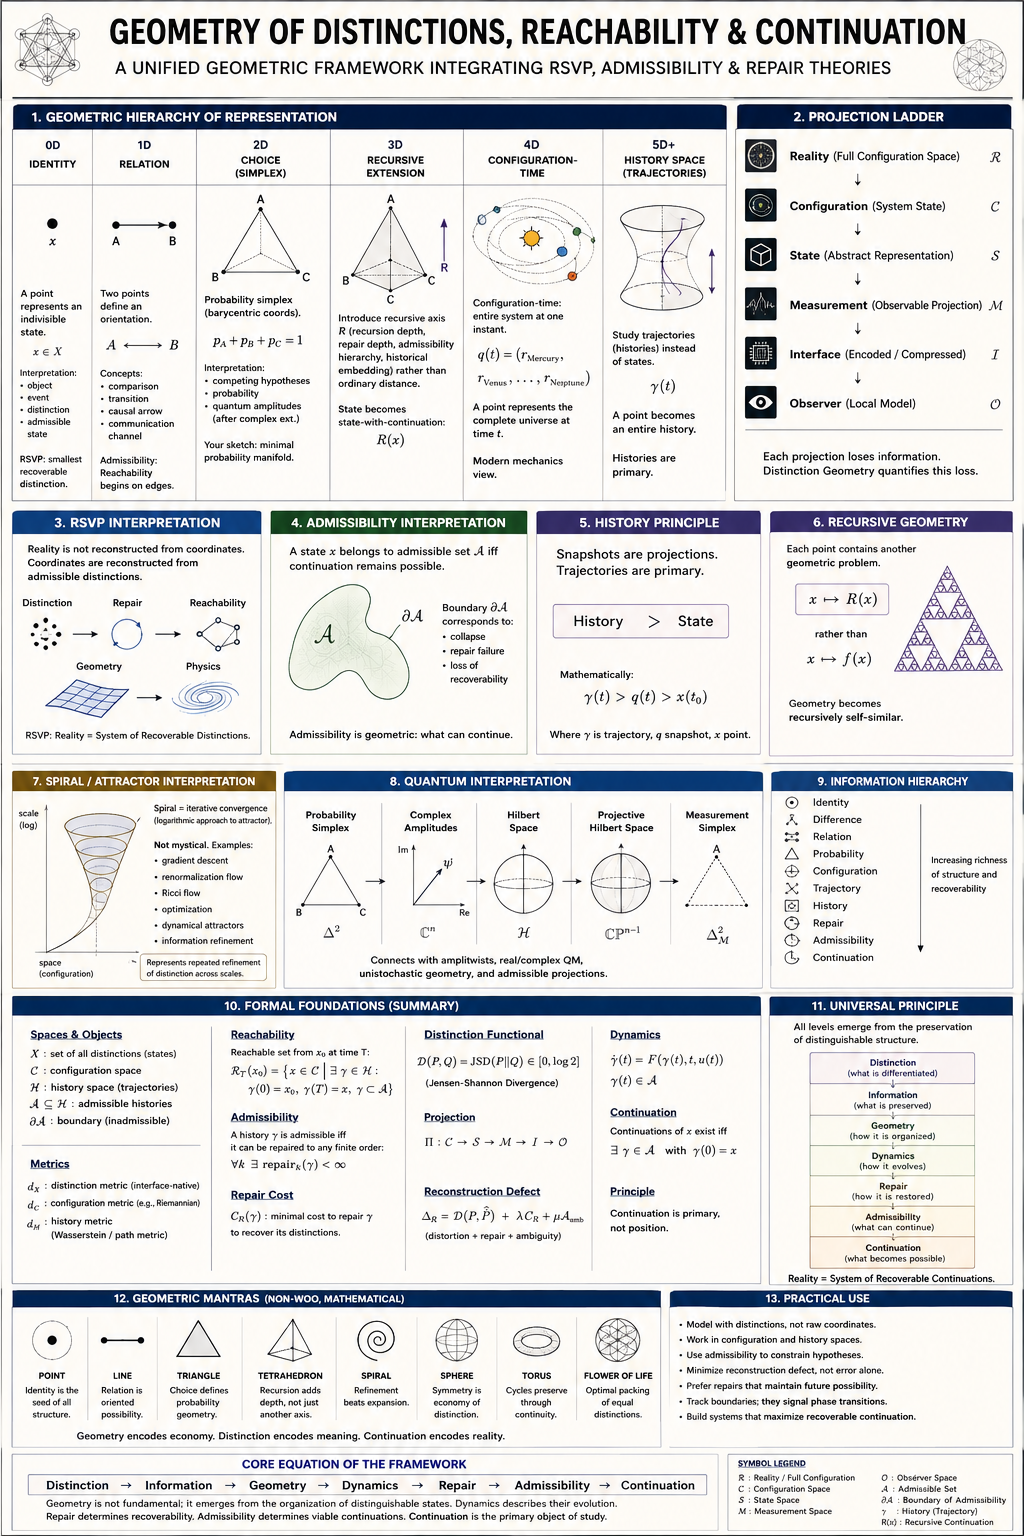
\includegraphics[width=0.7\textwidth]{figures/dependency-diagram.png}
\captionsetup{width=0.9\textwidth}
\caption{The dependency structure of Figure 1.1, reproduced without alteration. Every term it contains has now been given a definition: distinction (Chapter 6), constraint (Chapter 7), information (Chapter 8), repair (Chapters 9 and 13), admissibility (Chapters 10 and 15), continuation (Chapter 14), and the reachability, history, and boundary structure connecting them (Chapters 10, 11, and 22). The image has not changed since Chapter 1. What it is possible to read out of it has.}
\end{figure}

A reader returning to this diagram from Chapter 1 is now in a position to check it rather than merely admire it. Every arrow can be asked to justify itself against a specific chapter, and every box against a specific definition. This is offered as a test, not a summary: a diagram that only looked authoritative when unexplained was never doing any work; one that survives being checked, box by box, against four hundred pages of definitions, has earned the density it was given on page one.

\part{The Joke Explained}

\chapter{Why the Title Is Technically True}

The title of this book asserts a mathematical proof for the existence of God. Chapter 25 showed that no derivation in this book establishes that a mind, an agent, or a being capable of intention exists. On the ordinary reading of the title, then, the title is false, or at best wildly overstated, in exactly the way every argument surveyed in Chapter 2 turned out to be overstated.

There is a narrower reading under which the title is defensible, and this chapter states it precisely rather than leaving it to hover as an unexamined pun.

\begin{enumerate}
\item Under the hypotheses of Proposition 22.6, an object $G$ exists: Chapters 11 through 22 establish this by ordinary mathematical derivation, containing, by Theorem 22.9, no interpretive leap.
\item Definition 25.3 stipulates that the word ``God,'' if used in connection with this book at all, refers to $G$ and to the operator $T$ producing it.
\item Under that stipulation, and only under that stipulation, the sentence ``God exists'' is a restatement of Proposition 22.6, and is exactly as true as Proposition 22.6 is, which is to say: true given the stated hypotheses, and no stronger than that.
\end{enumerate}

This is the sense, and the only sense, in which the title is technically true. It is true the way it is technically true that a company's ``Chief Happiness Officer'' presides over happiness, if the title is granted and the further connotations of the words composing it are set aside. Nobody reading a job title that way is being fooled by it; nobody is expected to conclude that a corporation has certified the metaphysics of joy. The interesting cases, in both the corporate and the theological instance, are the readers who do draw the stronger conclusion, and Chapter 2 was, among other things, a survey of exactly how that stronger conclusion gets smuggled in when an author is less careful, or less honest, about where the stipulation sits.

A subtitle considered at an earlier stage of this project, and rejected, proposed calling the whole thing ``a proof in several incompatible notations.'' That phrase deserves a sentence here rather than a silent deletion, because the reason for rejecting it is the same reason this chapter has just given for the title it did keep. Several notations, none reducible to the others, each dressed with enough symbolic density to look load-bearing, is exactly the failure mode Chapter 4 spent its pages naming: apparent rigor multiplied by apparent independence, when the independence is the whole illusion. A book that actually wanted to prove something would need to pick one notation and hold every subsequent symbol answerable to it, which is what Chapters 6 through 22 do. The rejected subtitle would have advertised the crime this book was written to diagnose.

\chapter{The Mathematics Was the Easy Part}

Chapters 6 through 22 are long. They are not, in the main, difficult, once each definition is granted the one before it; a patient reader with the standards of Chapter 4 firmly in mind can check every proof in this book line by line, and every check will come out the same way, because every step was built to be checked. This is what a derivation is supposed to be: effortful to write, and comparatively mechanical to verify.

Chapters 23 through 25 took a fraction of the pages and none of the derivational apparatus, and they are, by a wide margin, the hardest part of this book, because they are the part no amount of additional derivation can make easier. Whether $T$ deserves the name it has been given in Definition 25.3, whether the terminus reading or the operator reading of Chapter 23 is the more faithful one, whether a clean glut at the seat of distinction counts as a mark against an interpretation or as exactly the kind of thing an apophatic tradition would have predicted, none of these questions yields to a longer proof. They are not questions a proof answers. They are questions a proof, at best, can be made to bear on, precisely and honestly, without pretending the bearing is itself an answer.

This asymmetry, four hundred pages of tractable derivation against three chapters of intractable interpretation, is not a flaw specific to this book. It is, this book has argued since Chapter 2, the shape of every serious attempt to derive something theological from something formal: the formal part is long and hard-won and, in the end, the least controversial thing in the room.

\chapter*{Open Problems}
\addcontentsline{toc}{chapter}{Open Problems}

A construction presented as though it were finished invites a different kind of reading than one presented as a stage in an ongoing program. This book has tried, throughout, to be honest about which it is; this chapter collects the specific places where the honest answer is that the mathematics runs out before the questions do.

\textbf{Classifying admissibility manifolds.} Chapter 15 equips $\partial \mathcal A$ with a metric and identifies phase points, but says nothing about the possible large-scale shapes $\partial \mathcal A$ can take. Whether admissibility manifolds admit a classification analogous to the classification of surfaces, or whether their possible geometries are as unconstrained as arbitrary metric spaces, is untouched by anything in this book.

\textbf{Characterizing the fixed points of $T$.} Proposition 21.4 characterizes fixed points of the global constraint operator abstractly, as worlds with nothing left for $T$ to repair, but gives no way to enumerate or parametrize the fixed points of a given $T$ short of checking each candidate world directly. A structural characterization, analogous to how the fixed points of a linear operator are characterized by its eigenspaces, is not attempted here.

\textbf{Infinite-dimensional and continuum worlds.} Every worked example in this book uses a finite $X$, and the finite case is where the master functional's existence-of-minimizer result (Proposition 16.3) is easiest to satisfy. Extending the theory to distinction spaces with infinitely many patches, or to continuum-many points, raises compactness questions this book's finite examples never had to face, and the extent to which Part IV's construction survives that extension is open.

\textbf{Stochastic repair.} Every repair operator in this book, $C_R$, the witness-repair cost $R(x,p)$, and $T$ itself, is deterministic: given a world, the repair, where it exists, is a specific map. A version in which repairs are chosen probabilistically, and admissibility is correspondingly a matter of degree rather than a binary property, would connect this book's apparatus to the case studies of the previous chapter, biological homeostasis in particular, far more directly than the present deterministic theory does.

\textbf{A categorical formulation.} The Neighboring Frameworks chapter noted, without developing, the resemblance between worlds and refinements on one hand and objects and morphisms on the other, with $T$ resembling an endofunctor and the cofinal limit resembling a colimit. Whether this resemblance survives being made precise, and what a category-theoretic treatment of admissibility would add beyond restating this book's results in different notation, is genuinely open.

\textbf{Relating repair geometry to probability.} Chapter 8 uses probability only to define information content and entropy on a fixed distribution; nothing in this book studies how repair costs behave under a probability measure on the space of possible degradations, which would be the natural setting for asking how likely a given world is to need repair at all, as opposed to how much a given repair costs once needed.

None of these problems is claimed to be original to this book in the sense of never having been considered under some other name in some other literature; several almost certainly have been. They are listed here because this book's specific formalism does not currently answer them, and a reader equipped with that formalism is better positioned to attempt them than a reader without it.

\chapter*{Predictions and Empirical Tests}
\addcontentsline{toc}{chapter}{Predictions and Empirical Tests}

This book is a work of mathematics, and mathematics alone does not predict anything about the world; a prediction requires an additional claim, that some real system is well modeled by the formalism, which is exactly the kind of interpretive step Chapter 2 taught this book to flag rather than assume. With that flag firmly in place, the following are the empirical-sounding claims the apparatus of this book would support, if a real system were shown to instantiate it in the sense of the Case Studies chapter.

A system with a higher local repair capacity, larger cost budgets available to $T$, should exhibit longer-lived local disagreement before that disagreement either resolves or forces a global incoherence, since Proposition 13.6's additivity means a system that can afford to repair several confounded gluts independently tolerates more simultaneous local disagreement than one that cannot. A system approaching the boundary of its admissibility manifold, in the sense of Definition 15.3's phase points, should show increased sensitivity to small perturbations, matching the general expectation, familiar from the study of phase transitions in physical systems, that systems become more fragile near a genuine boundary than deep within a stable region. A system whose repair operator is regularly forced to act on its own machinery rather than on ordinary local data, the autoimmune case from the Case Studies chapter, should show degraded ability to resolve ordinary local disagreements even when the immediate disagreement is unrelated to the affected machinery, since Chapter 21's operator $T$ is a single fixed construction whose own integrity is presupposed rather than separately guaranteed.

Each of these is a structural prediction, in the sense that it follows from the shape of the formalism rather than from any numerical parameter this book has fit to data, and none of them has been tested against a real system by this book. A reader in a position to test one is in a better position to judge this book's usefulness than any argument in Chapters 23 through 25 could put them in.

\begin{appendixremark}[A Biblical Analogy: Elijah and a Common Observational Test]
Two more analogies belong with this chapter's theme, offered, as before, as structural parallels rather than historical claims about what any ancient author understood by the word evidence. The contest on Mount Carmel (1 Kings 18) is notable for what Elijah does not do: he does not ask Israel to choose between Baal and YHWH by appeal to authority, ancestry, or rhetorical persuasion. He proposes instead a publicly observable test: two altars, prepared identically, two competing hypotheses, and a single shared observation to adjudicate between them. Unlike a modern experiment, the anticipated outcome is a miracle rather than a repeatable natural process, so this is not the scientific method in any methodologically modern sense; what it shares with that method is narrower and more structural, that competing explanations are made to answer to a common observational test, rather than being settled by argument about which is more plausible on its face.
\end{appendixremark}

\begin{appendixremark}[A Biblical Analogy: Gideon's Fleece and Independent Confirmation]
Gideon's fleece (Judges 6) tests something a single observation cannot: whether the proposed cause, rather than some unnoticed background asymmetry, is actually responsible for the result. Gideon first asks for the fleece to be wet while the ground around it stays dry; then, immediately, he reverses the request, fleece dry, ground wet. A single sign of either kind leaves room for an unconsidered natural explanation particular to that one arrangement. Reversing the conditions and checking that the explanation still predicts the outcome either way is structurally close to seeking independent confirmation rather than resting on one positive result, even though Judges 6 has nothing resembling replication by an independent party, a control group, or a quantified measurement, and the analogy should not be read as claiming otherwise.
\end{appendixremark}

\chapter*{Limitations}
\addcontentsline{toc}{chapter}{Limitations}

Stating a theory's boundaries plainly is worth more than letting a reader discover them by trial and error, and this book has occasion, by this point, to state several.

The theory throughout is binary at the level of admissibility: a state is in $A$ or it is not, at some finite or infinite repair distance. Every case study in this book that involves graded phenomena, physiological health, the gradual spread of a linguistic usage, has had to note this flattening explicitly. A graded or probabilistic generalization is listed as an open problem above and is not developed here.

The repair cost function $\mathrm{cost}$, on which nearly everything in Chapters 9 through 22 ultimately depends, is treated throughout as externally given: a fixed, theory-specific function this book never derives from more basic principles. A reader who wants to know where a particular cost function should come from, in a specific application, will not find an answer in this book; they will find a formalism that takes the answer as an input.

The master functional's constants $\lambda$ and $\mu$ (Definition 16.1) are likewise external parameters, fixed in advance rather than derived, and this book offers no principle for setting them beyond the qualitative monotonicity of Proposition 16.6. Two readers who disagree about how heavily to weight repair cost against coherence liability will not find that disagreement adjudicated here.

Several central results depend on hypotheses, compactness and semicontinuity in Proposition 16.3, admissibility-improvement and convergence in Proposition 22.6, that this book verifies in its own small worked examples but does not show how to verify in general. A reader applying this framework to a new domain inherits the burden of checking these hypotheses themselves; nothing in this book automates or guarantees that check.

Finally, and most importantly, the theological application of Chapters 23 through 25 is exactly as limited as Chapter 24 already says it is, and no later chapter, including this one, adds to that list. Restating the limitation here is not redundant; it is a reminder that a limitations chapter which excludes the book's own central application would be advertising rather than accounting.

\chapter{Q.E.D.*}

\begin{flushright}
\itshape ``A proof that refuses its own conclusion.''\\
\upshape --- N.G.
\end{flushright}

\bigskip

The apparatus is built. The object exists, given its hypotheses. The derivation contains no interpretive leap. The name has been chosen, and chosen openly, at the one place a name had to be chosen rather than proved.

\begin{center}
\Large \textbf{Q.E.D.*}
\end{center}

\vspace{0.5em}
\noindent\rule{4cm}{0.4pt}

\footnotesize
\noindent *Or at least as much as we're willing to check.
\normalsize

\part{Appendices}

\chapter*{Appendix A: Every Symbol Used}
\addcontentsline{toc}{chapter}{Appendix A: Every Symbol Used}

This appendix lists every symbol introduced in the main text, Chapters 1 through 25, grouped by the chapter in which it first appears, together with the definition that introduces it. Chapters 3, 4, 5, 23, 24, 26, 27, and 28 introduce no persistent notation of their own and are omitted below; their content is conceptual rather than symbolic, and is indexed instead in Appendix I.

\medskip
\noindent\textbf{Chapter 1: Every Proof Begins with a Definition}
\begin{description}
\item[$(L,A,R)$] Language, axioms, inference rules of a formal system (Definition 1.1).
\end{description}

\noindent\textbf{Chapter 2: Why Every Existing Proof Fails}
\begin{description}
\item[$\mathcal I$] Interpretation map, $\mathcal I : \mathcal F \to \mathcal M$ (Definition 2.2).
\end{description}

\noindent\textbf{Chapter 6: Distinction Before Objects}
\begin{description}
\item[$X$] Distinction space (Definition 6.1).
\item[$d_X$] Distinction metric (Definition 6.1).
\item[$\sim$] Distinguishing relation (Definition 6.4).
\item[$X/\!\sim$, $\bar d_X$] Quotient space and descended metric (Proposition 6.8).
\end{description}

\noindent\textbf{Chapter 7: Constraint Before Law}
\begin{description}
\item[$\mathcal C$] Constraint system (Definition 7.1).
\item[$A$] Jointly admissible set (Definition 7.1).
\item[$C_J$] Jointly admissible set of a sub-collection indexed by $J$ (Proposition 7.6).
\end{description}

\noindent\textbf{Chapter 8: Information Before Truth}
\begin{description}
\item[$P$] Probability distribution (Definition 8.1).
\item[$\mathrm{Info}_P$] Information content (Definition 8.1).
\item[$\mathrm{Ent}$] Entropy (Definition 8.1).
\item[$\mathcal D$] Jensen--Shannon distinguishability (Definition 8.5).
\end{description}

\noindent\textbf{Chapter 9: Repair Before Knowledge}
\begin{description}
\item[$C_R$] Repair cost (Definition 9.2).
\end{description}

\noindent\textbf{Chapter 10: Admissibility Before Reality}
\begin{description}
\item[$\mathcal H$, $\gamma$] History space and a history (Definition 10.1).
\item[$\mathcal A$] Admissible histories (Definition 10.1).
\item[$\partial \mathcal A$] Boundary of admissibility (Definition 10.4).
\end{description}

\noindent\textbf{Chapter 11: Worlds as Constraint Systems}
\begin{description}
\item[$W$] World (Definition 11.1).
\item[$U_i$, $U_{ij}$] Local patch and overlap of patches (Definitions 11.1, 11.2).
\item[$A_i$] Local admissible set of patch $U_i$ (Definition 11.2).
\end{description}

\noindent\textbf{Chapter 12: Witnesses}
\begin{description}
\item[$s^\pm$] Witness support, positive and negative (Definition 12.1).
\item[$q_i$] Local FDE value on patch $U_i$ (Definition 12.2).
\item[$\Sigma$, $\mathrm{Merge}_{FDE}$] Merged value and the FDE merge rule (Definition 12.3).
\item[$\delta^\pm$] Coherence defect (Definition 12.4).
\item[$\mathrm{Coh}^\pm$] Coherence of a proposition on an overlap (Definition 12.5).
\end{description}

\noindent\textbf{Chapter 13: Repair}
\begin{description}
\item[$R(x,p)$] Witness-repair cost of a confounded glut (Definition 13.2).
\end{description}

\noindent\textbf{Chapter 14: Continuations}
\begin{description}
\item[$\mathrm{Cont}(\gamma)$] Continuations of a history (Definition 14.1).
\item[$\mathcal R(\gamma)$] Reachable set (Definition 14.3).
\end{description}

\noindent\textbf{Chapter 15: Admissibility Geometry}
\begin{description}
\item[$d_{\mathcal A}$] Admissibility metric (Definition 15.1).
\end{description}

\noindent\textbf{Chapter 16: The Master Functional}
\begin{description}
\item[$E$, $R$, $C$, $J$] Ordinary cost, repair cost, coherence liability, master functional (Definition 16.1).
\item[$\lambda$, $\mu$] Repair and coherence weighting parameters (Definition 16.1).
\end{description}

\noindent\textbf{Chapter 17: Local Support}
\begin{description}
\item[$\mathrm{Dist}(U_i)$] Local distinction set of a patch (Definition 17.1).
\item[$\mathrm{Info}_i$, $<_i$] Local information and its induced order (Definition 17.2).
\end{description}

\noindent\textbf{Chapter 18: Coherence}
\begin{description}
\item[$\Sigma_W$] Global support, merged across every patch (Definition 18.1).
\end{description}

\noindent\textbf{Chapter 19: Gluts Without Explosion}
\begin{description}
\item[$\vdash_{FDE}$] Glut-safe inference relation (Definition 19.1).
\end{description}

\noindent\textbf{Chapter 20: Reconstruction}
\begin{description}
\item[$W'$] Partial world (Definition 20.1).
\item[$\Delta_R$] Reconstruction defect (Definition 20.2).
\end{description}

\noindent\textbf{Chapter 21: The Global Constraint Operator}
\begin{description}
\item[$T$] Global constraint operator (Definition 21.1).
\end{description}

\noindent\textbf{Chapter 22: The Cofinal Limit}
\begin{description}
\item[$W^\uparrow$] Refinement of a world (Definition 22.1).
\item[$W_\infty$] Cofinal limit of a refinement chain (Definition 22.3).
\item[$G$] The terminal object, $G := W_\infty$ (Definition 22.10).
\end{description}

\noindent\textbf{Chapter 25: The Semantic Leap}
\begin{description}
\item[$\mathcal I_{\mathrm{theo}}$] The interpretation sending $G$ or $T$ to the domain of the word ``God'' (Definition 25.1).
\end{description}

\begin{appendixremark}
Grouping by chapter rather than alphabetizing was a deliberate choice, corrected into this appendix from an earlier, denser paragraph form after a reviewer pointed out the obvious: a reader who forgets what $d_{\mathcal A}$ means is helped more by being told it belongs to the admissibility-geometry chapter than by an alphabetical listing under $d$. It also mirrors the construction order this book has insisted on since Chapter 6, so that the index itself is a compressed restatement of the dependency chain rather than an alphabetized escape from it. Appendices J through Z introduce their own local notation, documented within each appendix where it is defined rather than duplicated here.
\end{appendixremark}

\chapter*{Appendix B: Frequently Misunderstood Equations}
\addcontentsline{toc}{chapter}{Appendix B: Frequently Misunderstood Equations}

Several equations in this book resemble familiar mathematical expressions while carrying a more limited or more specific meaning than readers sometimes assume. This appendix collects the most common sources of confusion and states, explicitly, what each equation does and does not assert.

\section*{$G := W_\infty$}

The expression $G := W_\infty$ (Definition 22.10) is a stipulative definition in exactly the sense formalized in Chapter 5. It is not an equation asserting that two independently existing mathematical objects have been shown to coincide. Prior to Definition 22.10 there is no symbol $G$ in the formal language of this book; the definition introduces the letter $G$ as an abbreviation for the object already constructed and already proved to exist, the cofinal limit $W_\infty$.

Everything proved about $G$ could be rewritten by replacing every occurrence of $G$ with $W_\infty$ without changing a single theorem. The definition introduces no new mathematical content, no new existence theorem, and no additional properties beyond those $W_\infty$ already has. A reader who finds themselves thinking that this line ``creates'' anything should reread Chapter 5, whose central point is precisely that names do not generate existence; the work establishing existence (Proposition 22.6) and uniqueness (Proposition 22.7, under the hypothesis that $W_0$'s cover already covers $X$, stated in full in Chapter 22) is complete before the symbol $G$ is introduced at all.

\section*{$T(G) = G$}

Proposition 23.1 states $T(G) = G$. This is frequently misread as asserting that $G$ is static, frozen, or incapable of change; neither the proposition nor its proof supports that reading. The proposition asserts only that $G$ is a fixed point of the specific operator $T$ built in Definition 21.1: applying $T$ again produces no further reconstruction. Nothing in Proposition 23.1 says that every process internal to $G$ is stationary, or that any notion of local change within $G$, to the extent this book's formalism supports one, ceases. Indeed $T$ generally transforms every other world, $T(W) \neq W$ for a generic $W$; the proposition identifies one world at which this particular reconstruction process has reached closure, in the same sense a Banach fixed point, an equilibrium solution of a differential equation, or a terminal object in category theory is a point of closure for the operation defining it, not a claim that time or process has stopped anywhere.

\section*{$\Sigma_W(p)(x) = B$}

Definition 18.1 introduces the global support $\Sigma_W(p)(x)$, valued in the four-element set $\{T,F,B,N\}$ first fixed in Definition 12.2. The value $\Sigma_W(p)(x) = B$ is likely the single most misread equation in this book. It does not mean that $p$ is false, that an error has occurred, that reasoning has collapsed, or that every proposition becomes provable. It states only that, within the witness structure available to $W$, admissible support exists both for $p$ and for $\neg p$ at $x$, in the sense fixed by Definition 12.5. This is the ordinary reading of a glut in first-degree entailment, the paraconsistent logic this book adopts from Chapter 12 onward specifically because it rejects the classical rule of explosion, Chapter 19's Proposition 19.2, so that a glut need not trivialize anything beyond the proposition it occurs at. Chapters 12 and 13 further distinguish a clean glut, one whose opposing support is not attributable to any patch disagreement the theory can locate and is therefore not repairable, from a confounded one, which is. $\Sigma_W(p)(x) = B$ by itself asserts only the first half of that distinction; whether the glut is clean or confounded is a separate fact, established or refuted by Definition 12.5's further conditions, not by the bare value $B$ alone.

\section*{$C_R(x) = \infty$}

Definition 9.2 defines the repair cost $C_R(x)$. When $C_R(x) = \infty$, this is often read informally as asserting that repair is impossible in some absolute sense. The definition is narrower: it means only that no repair map exists within the specific class of repair maps this book's formalism admits, fixed once and for all in Chapter 9. A reader who enlarges that class, by admitting repair maps this book did not consider, could in principle find some previously irrecoverable point becomes recoverable under the enlarged class; the symbol $\infty$ therefore records a fact about the formal system as given, not a metaphysical claim about what can never, under any elaboration of the theory, be undone.

\section*{$\partial \mathcal A$}

The notation $\partial \mathcal A$ (Definition 10.4) is borrowed from topology, and readers should resist importing every property ordinarily associated with a topological boundary along with the symbol. Definition 10.4 specifies exactly one thing: the set of points at which every neighborhood contains both a state extendable to an admissible history and a state that is not. Whether this boundary is connected, smooth, compact, or possesses any further geometric structure depends entirely on hypotheses supplied later, chiefly in Chapter 15, and should never be assumed merely because the symbol $\partial$ suggests a family resemblance to boundaries studied elsewhere.

\section*{A General Principle}

Every misunderstanding collected in this appendix has the same source. Each equation's symbols resemble notation from other branches of mathematics, logic, or theology closely enough that a reader can supply a meaning from that other context before checking the definition that actually introduced the symbol in this one. This book's own standard, stated plainly since Chapter 4, runs the opposite direction: definitions determine meaning, and notation, however familiar it looks, does not. Whenever an equation in this book seems to be claiming more than it should, the reliable procedure is the slow one: return to the definition that introduced each symbol in the expression, substitute that definition back in, and only then ask what has actually been established. This is not a shortcut available only to the confused; it is the same procedure by which every proof in this book was checked before it was allowed to appear in it.

\chapter*{Appendix C: Things This Book Does Not Claim}
\addcontentsline{toc}{chapter}{Appendix C: Things This Book Does Not Claim}

This book does not claim to have proved the existence of a conscious being. It does not claim that any religious tradition is correct, incorrect, or approximately correct. It does not claim that prayer, ritual, or worship are efficacious, appropriate, or misguided. It does not claim that $G$ or $T$ has preferences, issues commands, or grounds moral obligation. It does not claim that atheism is false. It does not claim that theism is true. It does not claim that its own central definitional choice, Definition 25.3, is forced on a reader by anything preceding it. The full statement of what is and is not claimed appears in Chapter 24; this appendix exists only for readers who skipped ahead.

\chapter*{Appendix D: A Completely Different Proof (Which Also Fails)}
\addcontentsline{toc}{chapter}{Appendix D: A Completely Different Proof (Which Also Fails)}

Let $\mathcal U$ be the set of physical constants of the observed universe. It is a matter of ordinary physics that small perturbations to many members of $\mathcal U$ would preclude the formation of stable atoms, stars, or chemistry adequate to sustain observers. Call this fact fine-tuning. Let $\mathcal D$ be a probability distribution over possible values of $\mathcal U$ under which the observed values are assigned low probability. Define $\mathcal G := $ ``whatever selected $\mathcal U$ from among the values $\mathcal D$ disfavors.''

This argument is included as a specimen, not a rival. Its formal content, that the observed constants are low-probability under a stated distribution, is real and checkable, in exactly the sense Chapter 2 credited to the strongest steps of the arguments surveyed there. Its failure is exactly Chapter 2's diagnosis: nothing in the specification of $\mathcal D$ or the fact of fine-tuning licenses the further move from ``selected'' to ``selected by an agent,'' and the definition of $\mathcal G$ smuggles that agency in through the verb rather than establishing it. An anthropic selection effect, a prior stage of cosmological evolution favoring life-permitting regions, and an intentional designer are, prior to further argument, equally consistent with $\mathcal D$ disfavoring the observed values; $\mathcal G$'s definition does not distinguish among them, and no amount of additional precision about $\mathcal D$ will make it do so, for the same reason no amount of additional precision about $\mathrm{Merge}_{FDE}$ would have licensed Definition 25.1 on its own.

\chapter*{Appendix E: If You Read This as Theology}
\addcontentsline{toc}{chapter}{Appendix E: If You Read This as Theology}

Read as theology, this book belongs to the apophatic and immanentist traditions more than to classical theism: it approaches its terminal object through negation and structural role rather than through positive attribution of power or personality, and it locates that object within the system it describes rather than prior to or outside it, in the manner of Spinoza more than of the Abrahamic creator traditions. Readers drawn to this reading are asked to take Chapter 24's list of what is not established as seriously as its list of what is; a theology built on this book's construction inherits its restraint along with its structure, or it is not built on this book's construction.

\chapter*{Appendix F: If You Read This as Satire}
\addcontentsline{toc}{chapter}{Appendix F: If You Read This as Satire}

Read as satire, this book's target is not belief, disbelief, or any particular religious tradition, but a specific rhetorical move: the construction of enough formal machinery that a reader, exhausted by the checking, accepts the terminal definition without checking it as carefully as the definitions that came before it. Every chapter of Part I named this move before Part II ever began building anything for it to be tried on; every subsequent part built the machinery anyway, honestly, and then tried the move on the reader exactly once, in Chapter 25, in the open, with its own name attached. Whether that counts as having avoided the move or as having performed it in the least deniable way available is, itself, a question this book declines to adjudicate, for reasons Chapter 23 already gave.



\chapter*{Appendix G: Glossary of Terms}
\addcontentsline{toc}{chapter}{Appendix G: Glossary of Terms}

\textbf{Admissibility.} The property of a state or history of satisfying, or being repairable back to, the constraint structure in force; formalized as membership in $\mathcal A$ (Definition 10.1).

\textbf{Admissibility manifold.} The boundary $\partial\mathcal A$ equipped with the admissibility metric $d_{\mathcal A}$, treating admissibility geometrically rather than merely combinatorially (Definition 15.3).

\textbf{Clean glut.} A point at which a world's own witness data, in full agreement across every patch that speaks to the question, supports both a proposition and its negation; not an error, and not repairable without discarding genuine support (Definition 12.5, Proposition 13.3).

\textbf{Coherence defect.} A measure of whether two patches agree on a point's positive or negative support for a proposition; zero exactly when they agree (Definition 12.4).

\textbf{Confounded glut.} A glut arising from disagreement between patches rather than from any single patch's own overdetermined data; repairable, unlike a clean glut (Definition 12.5).

\textbf{Constraint.} A subset of a distinction space ruling certain configurations in and others out; a law, on this book's account, is simply a constraint whose violation has not been observed (Definition 7.1).

\textbf{Continuation.} An admissible extension of a history beyond a given point (Definition 14.1).

\textbf{Cover.} A family of patches whose union is the whole distinction space, from which a world's local constraint data is assembled (Definition 11.1).

\textbf{Distinction.} An element of a distinction space, available to be told apart from other elements by a distinction metric; the primitive this book builds everything else from (Chapter 6).

\textbf{FDE (first-degree entailment).} The four-valued logic, due to Belnap and Dunn, whose values $T$, $F$, $B$, $N$ (true, false, both, neither) this book uses to record witness data without collapsing disagreement or silence into error (Definition 12.2).

\textbf{Glut.} A point at which a proposition's merged support value is $B$: both witnessed true and witnessed false (Definition 12.5).

\textbf{Interpretive leap.} A step in a derivation that depends on an interpretation of a symbol not licensed by the formal system's own inference rules; the central diagnostic tool of this book (Definition 2.3).

\textbf{Master functional.} $J(a) = E(a) + \lambda R(a) + \mu C(a)$, balancing ordinary cost against repair cost and coherence liability for a given transition (Definition 16.1).

\textbf{Reconstruction defect.} The minimal cost of extending a partial world to a globally admissible one, combining missing-data repair and confounded-glut repair (Definition 20.2).

\textbf{Refinement.} A world built on a finer cover than another, agreeing with it wherever both are defined; a refinement chain is the sequence of successive repairs whose limit, under stated conditions, is $G$ (Definition 22.1).

\textbf{Repair.} A map returning a degraded or confounded element to admissibility, at some cost; repair cost measures distance from admissibility rather than an independent quantity (Chapter 9, Chapter 13).

\textbf{Self-witnessing.} A distinction space in which the distinguishing relation $\sim$ itself falls within the domain of a proposition asking whether it is a distinction, producing the book's central self-referential clean glut (Definition 19.3).

\textbf{Stipulative definition.} A definition introducing a symbol as an abbreviation, adding no new theorems beyond what substitution already permits, and in particular never establishing existence on its own (Definition 5.1).

\textbf{Witness.} A pair of subsets of a patch recording that patch's positive and negative support for a proposition (Definition 12.1).

\textbf{World.} A cover of a distinction space together with local constraint data on each patch, not assumed in advance to cohere globally (Definition 11.1).

\chapter*{Appendix H: Mathematical Background}
\addcontentsline{toc}{chapter}{Appendix H: Mathematical Background}

This appendix collects, in one place, the standard mathematical material this book draws on. None of it is original to this book; it is included so that a reader unfamiliar with one of these areas does not need an outside reference to follow the main text. Readers already comfortable with metric spaces, elementary order theory, many-valued logic, and Shannon information theory can skip directly to Chapter 6.

\section*{Sets, Relations, and Order}

A \emph{relation} $R$ on a set $X$ is a subset of $X \times X$; we write $xRy$ for $(x,y) \in R$. A relation is \emph{reflexive} if $xRx$ for all $x$, \emph{symmetric} if $xRy$ implies $yRx$, and \emph{transitive} if $xRy$ and $yRz$ imply $xRz$. An \emph{equivalence relation} is reflexive, symmetric, and transitive; it partitions $X$ into disjoint \emph{equivalence classes}, and the set of classes is the \emph{quotient} $X/R$, with $[x]$ denoting the class containing $x$. This book's distinguishing relation $\sim$ (Definition 6.4) is an equivalence relation constructed from a distinction metric, and the quotient $X/\!\sim$ (Definition 6.4) is an ordinary equivalence-class quotient.

A \emph{partial order} is a reflexive, transitive relation that is also \emph{antisymmetric} ($xRy$ and $yRx$ imply $x=y$); a \emph{strict partial order} $<$ additionally satisfies irreflexivity ($x \not< x$) in place of reflexivity. A partial order is \emph{total} if every two elements are comparable; otherwise some pairs are \emph{incomparable}. A set equipped with a partial order is a \emph{poset}. Every finite nonempty poset has at least one \emph{minimal element}, an element with nothing strictly below it (Proposition 17.6 uses this fact directly). These notions underlie Chapter 17's information ordering $<_i$, which is a strict partial order but generally not total (Proposition 17.3).

\section*{Metric and Distinction Spaces}

A \emph{metric} on a set $X$ is a function $d: X \times X \to \mathbb R_{\geq 0}$ satisfying $d(x,x)=0$, $d(x,y)=0 \implies x=y$, symmetry, and the triangle inequality $d(x,z) \leq d(x,y)+d(y,z)$. A \emph{pseudometric} drops the requirement that $d(x,y)=0$ forces $x=y$. This book's distinction metric $d_X$ (Definition 6.1) is weaker still, requiring only $d_X(x,x)=0$; Proposition 6.10 shows that adding symmetry and the triangle inequality recovers an ordinary metric on the quotient $X/\!\sim$.

An open \emph{cover} of a set $X$ is a family of subsets $\{U_i\}$ with $X = \bigcup_i U_i$; the \emph{overlap} of two members is their intersection. A central concern of elementary sheaf theory and of ordinary topology alike is when data specified locally, patch by patch, can be assembled (``glued'') into a single global object, and precisely when it cannot, because two patches disagree on an overlap. This is exactly the concern of Chapter 11: a world's local admissible sets can each be individually consistent while disagreeing on an overlap, precisely blocking global assembly (Proposition 11.4), and agreement on every overlap is what licenses gluing to a unique global set (Proposition 11.6, the Gluing Theorem). Readers who have seen sheaf-theoretic gluing conditions before will recognize the pattern; readers who have not will find Chapter 11 self-contained.

\section*{Many-Valued and Paraconsistent Logic}

Classical propositional logic assigns each proposition exactly one of two values, true or false, and includes the rule of \emph{explosion} (ex falso quodlibet): from a contradiction $p \wedge \neg p$, any conclusion whatsoever follows. \emph{First-degree entailment} (FDE), introduced by Belnap and Dunn to model reasoning from possibly incomplete or possibly conflicting sources, instead assigns each proposition one of four values: $T$ (true only), $F$ (false only), $B$ (both true and false, a \emph{glut}), and $N$ (neither, a \emph{gap}). A value is \emph{designated} if it counts as an acceptable premise, ordinarily $\{T,B\}$. A logic is \emph{paraconsistent} if it does not validate explosion: a contradiction at one proposition need not license arbitrary conclusions elsewhere. Chapter 19 builds a paraconsistent inference relation $\vdash_{FDE}$ for exactly this reason (Proposition 19.2, No Explosion), and Chapter 19's self-witnessing construction (Definition 19.3, Proposition 19.4) is this book's central application of a genuine, non-explosive glut. Graham Priest's dialetheism is the philosophical position that some such gluts are not mere modeling artifacts but describe how the world, or a formal system's best account of it, actually is; this book does not adopt dialetheism as a thesis, but its formalism is built to accommodate a genuine glut without collapse should one arise, as one does at Chapter 19's self-witnessing relation $\sim$.

\section*{Information Theory}

Given a probability distribution $P$ on a finite or countable set $X$, the \emph{information content} (or \emph{surprisal}) of an outcome $x$ is $\mathrm{Info}_P(x) := -\log_2 P(x)$, and the \emph{Shannon entropy} of $P$ is $\mathrm{Ent}(P) := -\sum_x P(x)\log_2 P(x)$, the expected information content. Entropy is minimized, at zero, exactly by point masses, and maximized by the uniform distribution (Proposition 8.7). The \emph{Kullback--Leibler divergence} $\mathrm{KL}(P\|Q) := \sum_x P(x)\log_2\frac{P(x)}{Q(x)}$ measures how much a distribution $P$ diverges from a reference $Q$; it is always nonnegative (Gibbs' inequality) but not symmetric. The \emph{Jensen--Shannon divergence} $\mathrm{JSD}(P\|Q) := \tfrac12\mathrm{KL}(P\|M) + \tfrac12\mathrm{KL}(Q\|M)$, with $M := \tfrac12(P+Q)$, symmetrizes this and is bounded, $0 \leq \mathrm{JSD}(P\|Q) \leq \log 2$ (Proposition 8.10). This book uses information content and entropy (Definition 8.1) to order distinctions by how much a given model expects them, explicitly prior to and independent of any notion of truth (Chapter 8's title and central claim), and uses Jensen--Shannon divergence (Definition 8.5) to extend the book's distinction metric from pairs of points to pairs of probabilistic models.

\section*{Optimization and Semicontinuity}

Optimization problems ask whether a quantity can be made as small, or as large, as possible within some prescribed class of admissible objects. The distinction between the existence of an infimum and the existence of an actual minimizer is one of the oldest themes in analysis, and nearly every existence theorem in the calculus of variations, optimal control, and nonlinear optimization ultimately reduces to identifying hypotheses under which minimizing sequences converge to genuine solutions rather than escaping to infinity or oscillating indefinitely without settling.

The hypothesis most commonly used for this purpose is \emph{lower semicontinuity}. A function $f : X \to \mathbb R \cup \{\infty\}$ on a topological or metric space is lower semicontinuous if, for every $x \in X$, $\liminf_{y \to x} f(y) \geq f(x)$: the function cannot suddenly jump downward in the limit, though it may jump upward. Equivalently, every sublevel set $\{x \in X : f(x) \leq c\}$ is closed for every $c \in \mathbb R$, a characterization frequently more useful in optimization, since a minimizing sequence then stays trapped inside a closed sublevel set rather than escaping through a limit point lying outside it.

Compactness supplies the second ingredient: it prevents a minimizing sequence from escaping indefinitely without converging at all, since every sequence in a compact space has a convergent subsequence, and lower semicontinuity then guarantees the limit's value is no larger than what the sequence was already approaching. Combining the two gives one of the standard existence results of analysis: a lower semicontinuous function on a nonempty compact space attains its infimum. The result appears in many equivalent forms throughout real analysis, the direct method of the calculus of variations, nonlinear programming, and optimal transport; every proof, however it is presented, combines compactness with lower semicontinuity to rule out a minimizing sequence either escaping the domain or converging to a point whose value exceeds the infimum it was supposed to be approaching.

The master functional $J = E + \lambda R + \mu C$ of Definition 16.1 is built so that this standard result applies directly. Its three constituents, ordinary transition cost, repair cost, and coherence liability, are each assumed, under Proposition 16.3's stated hypotheses, to be lower semicontinuous on the admissible space of transitions; since a nonnegative combination of lower semicontinuous functions is again lower semicontinuous, $J$ inherits the property immediately, and compactness of the admissible transition space then yields at least one cost-minimizing transition. Nothing in this argument is specific to this book's theological application; Proposition 16.3 is an ordinary optimization theorem, differing from a textbook existence proof only in which particular quantities have been combined into the objective functional.

The hypotheses matter precisely because they specify what happens when existence fails. Without compactness, a minimizing sequence may drift toward infinity without converging. Without lower semicontinuity, a sequence may converge while its limit's cost strictly exceeds the infimum the sequence was approaching, so that the optimum is approached but never attained; neither failure is exotic, and both occur routinely in ordinary optimization. Part IV accordingly never assumes every admissible optimization problem has an attained minimizer. Where Proposition 16.3's hypotheses do not hold, the construction proceeds by replacing minimizers with infima and building refinement chains whose costs converge monotonically toward the optimal value, the same accommodation modern optimization theory makes wherever compactness or semicontinuity is unavailable: relaxed solutions and convergent minimizing sequences standing in for an optimum that may not, strictly, be attained.

Proposition 16.3 is therefore best understood not as an isolated technical lemma but as the point where this book's own construction connects to one of analysis's standard existence principles, inheriting both its power and its limits: minimize genuine functions on well-behaved spaces where the hypotheses hold, and work with limits of increasingly good approximations, rather than an assumed optimum, wherever they do not.

\chapter*{Appendix I: Index of Definitions, Propositions, and Theorems}
\addcontentsline{toc}{chapter}{Appendix I: Index of Definitions, Propositions, and Theorems}

This index lists every numbered definition, proposition, theorem, lemma, corollary, remark, and example in Chapters 1 through 25, in order, with a short description. It is meant for readers who recall a result's content but not its number, or who want to trace which chapters build on which.

\needspace{5\baselineskip}
\subsection*{Chapter 1: Every Proof Begins with a Definition}
Definition 1.1 (formal system); Definition 1.2 (interpretation of a formal system); Remark 1.3 (ontological arguments as interpretive disputes).

\needspace{5\baselineskip}
\subsection*{Chapter 2: Why Every Existing Proof Fails}
Proposition 2.1 (reconstruction of the CTMU argument, self-referential closure); Definition 2.2 (interpretation map $\mathcal I:\mathcal F\to\mathcal M$); Definition 2.3 (Interpretive Leap); Proposition 2.4 (every surveyed argument contains a proper sub-derivation plus one leap).

\needspace{5\baselineskip}
\subsection*{Chapter 3: The Same Leap, Elsewhere}
Remark 3.1 (expected-value fanaticism parallels Pascal's Wager).

\needspace{5\baselineskip}
\subsection*{Chapter 4: The Dangerous Power of Symbols}
Definition 4.1 (load-bearing symbolic expression); Proposition 4.2 (rhetorical force is not a function of logical strength).

\needspace{5\baselineskip}
\subsection*{Chapter 5: Naming Is Not Explaining}
Definition 5.1 (stipulative definition); Remark 5.2 (stipulation alone does not entail existence); Proposition 5.3 (satisfiability of $\varphi$ does not entail $\exists x\,\varphi(x)$).

\needspace{5\baselineskip}
\subsection*{Chapter 6: Distinction Before Objects}
Definition 6.1 (distinction space $(X,d_X)$); Definition 6.2 (distinguishable / distinction); Remark 6.3 (points as a special case of distinction); Definition 6.4 (distinguishing relation $\sim$); Remark 6.5 (symmetry of $\sim$ is a real constraint on $d_X$); Lemma 6.6 ($\sim$ is reflexive); Remark 6.7 (transitivity of $\sim$ is not automatic); Proposition 6.8 (quotient $d_X$ descends to $\bar d_X$, under symmetry and the triangle inequality); Example 6.9 (three-point distinction space); Proposition 6.10 (quotient is a metric under symmetry + triangle inequality); Remark 6.11 (scope of the metric upgrade).

\needspace{5\baselineskip}
\subsection*{Chapter 7: Constraint Before Law}
Definition 7.1 (constraint, constraint system, jointly admissible set); Definition 7.2 (consistent / inconsistent constraint system); Lemma 7.3 ($A \cap B \subseteq A$); Proposition 7.4 (enlarging a constraint system shrinks the admissible set); Remark 7.5 (law as an unviolated constraint); Proposition 7.6 ($J\mapsto C_J$ is antitone); Example 7.7 (four-element inconsistency example).

\needspace{5\baselineskip}
\subsection*{Chapter 8: Information Before Truth}
Definition 8.1 (information content, entropy); Lemma 8.2 (log of a product); Proposition 8.3 (information and entropy add across independent distinctions); Remark 8.4 (why the logarithm specifically); Definition 8.5 (Jensen--Shannon distinguishability $\mathcal D$); Remark 8.6 ($\mathcal D$ extends $d_X$ to distributions); Proposition 8.7 (entropy vanishes iff point mass, maximized iff uniform); Proposition 8.8 ($\mathrm{Info}_P(x)\geq0$); Example 8.9 (biased-coin entropy computation); Proposition 8.10 ($\mathcal D$ symmetric and bounded by $\log 2$).

\needspace{5\baselineskip}
\subsection*{Chapter 9: Repair Before Knowledge}
Definition 9.1 (degradation, repair); Definition 9.2 (repair cost $C_R$); Remark 9.3 (infimum, not minimum); Proposition 9.4 ($C_R(x)=0$ on $A$); Definition 9.5 (recoverable / irrecoverable); Remark 9.6 (recoverability independent of any agent); Lemma 9.7 (composition of repairs is a repair); Proposition 9.8 (subadditivity of repair cost under composition); Example 9.9 (real-line repair-cost example).

\needspace{5\baselineskip}
\subsection*{Chapter 10: Admissibility Before Reality}
Definition 10.1 (history, admissible history, $\mathcal A$); Proposition 10.2 (admissibility relative to $A$ implies admissibility relative to any $B \supseteq A$); Example 10.3 (converse fails); Definition 10.4 (boundary $\partial\mathcal A$); Proposition 10.5 (boundary points are irrecoverable or marginally recoverable); Remark 10.6 (boundary as locus of marginal recoverability); Definition 10.7 (reality as the pair $(X,\mathcal A)$); Example 10.8 (restricted-repair real-line example); Proposition 10.9 ($\partial\mathcal A=\{-2,2\}$ in that example).

\needspace{5\baselineskip}
\subsection*{Chapter 11: Worlds as Constraint Systems}
Definition 11.1 (cover, world); Definition 11.2 (overlap, local admissible set); Definition 11.3 (locally / globally admissible); Proposition 11.4 (local admissibility does not imply global admissibility); Remark 11.5 (overlap disagreement is the seed of Part III); Proposition 11.6 (Gluing Theorem); Corollary 11.7 (global admissibility iff overlap agreement); Remark 11.8 (why Chapter 12's apparatus is the only place gluing can fail); Example 11.9 (agreeing overlaps glue uniquely).

\needspace{5\baselineskip}
\subsection*{Chapter 12: Witnesses}
Definition 12.1 (witness $(s_i^+,s_i^-)$); Definition 12.2 (local FDE value $q_i(p)$); Definition 12.3 (merged value $\Sigma$, $\mathrm{Merge}_{FDE}$); Definition 12.4 (coherence defect $\delta^\pm$); Definition 12.5 (coherent, glut, clean/confounded glut); Remark 12.6 (coherence is overlap-wide, not pointwise); Proposition 12.7 (the Ch.11 world has a confounded glut); Remark 12.8 (clean vs. confounded gluts call for different responses); Example 12.9 (full $\mathrm{Merge}_{FDE}$ computation); Proposition 12.10 ($\mathrm{Merge}_{FDE}$ is a commutative idempotent monoid).

\needspace{5\baselineskip}
\subsection*{Chapter 13: Repair}
Definition 13.1 (witness repair); Definition 13.2 (repair cost of a confounded glut $R(x,p)$); Proposition 13.3 (clean gluts cannot be witness-repaired); Remark 13.4 (repair is right for confounded gluts only); Example 13.5 (repair cost $=1$ for the running example); Proposition 13.6 (additivity of repair cost across independent gluts).

\needspace{5\baselineskip}
\subsection*{Chapter 14: Continuations}
Definition 14.1 (continuation, $\mathrm{Cont}(\gamma)$); Proposition 14.2 ($\mathrm{Cont}(\gamma)\neq\emptyset$ iff $\gamma$ admissible); Definition 14.3 (reachable set $\mathcal R(\gamma)$); Proposition 14.4 (points of $\mathcal R(\gamma)$ are admissible or recoverable); Example 14.5 (finite reachable-set example); Proposition 14.6 ($\mathcal R(\gamma')\subseteq\mathcal R(\gamma)$ under continuation).

\needspace{5\baselineskip}
\subsection*{Chapter 15: Admissibility Geometry}
Definition 15.1 (admissibility metric $d_{\mathcal A}$); Proposition 15.2 ($(X,d_{\mathcal A})$ is a distinction space); Definition 15.3 (admissibility manifold, phase point); Remark 15.4 (phase points as failure of local boundedness); Example 15.5 ($d_{\mathcal A}$ computed numerically); Proposition 15.6 (identifying a phase point vs. a non-phase point).

\needspace{5\baselineskip}
\subsection*{Chapter 16: The Master Functional}
Definition 16.1 ($E$, $R$, $C$, master functional $J$); Proposition 16.2 ($J=E$ absent repair/coherence burden); Proposition 16.3 (Existence of a minimizer); Remark 16.4 (scope of the minimizer hypotheses); Example 16.5 (full numeric $J(a)=1.3$ computation); Proposition 16.6 ($J$ nondecreasing in $\lambda,\mu$).

\needspace{5\baselineskip}
\subsection*{Chapter 17: Local Support}
Definition 17.1 (local distinction set $\mathrm{Dist}(U_i)$); Definition 17.2 (local information, order $<_i$); Proposition 17.3 ($<_i$ is a strict partial order, not total); Remark 17.4 (incomparability is a real feature, not a defect); Example 17.5 (incomparable-distinctions example); Proposition 17.6 (finite nonempty posets have a minimal element).

\needspace{5\baselineskip}
\subsection*{Chapter 18: Coherence}
Definition 18.1 (global support $\Sigma_W(p)$); Lemma 18.2 ($\mathrm{Merge}_{FDE}$ is commutative and associative); Proposition 18.3 ($\Sigma_W$ independent of merge order); Definition 18.4 (globally coherent world); Proposition 18.5 (global coherence precludes confounded gluts); Example 18.6 (three-patch associativity computation); Proposition 18.7 (coherence criterion absent single-patch gluts).

\needspace{5\baselineskip}
\subsection*{Chapter 19: Gluts Without Explosion}
Definition 19.1 (glut-safe inference $\vdash_{FDE}$); Proposition 19.2 (No Explosion); Definition 19.3 (self-witnessing distinction space); Proposition 19.4 ($\sim$ has a clean glut at itself); Remark 19.5 (the self-distinguishing question resolved as a real glut); Remark 19.6 (Proposition 19.4's own proof is an interpretive leap, named as one); Example 19.7 (explicit two-point no-explosion instance); Proposition 19.8 ($\vdash_{FDE}$ is reflexive and monotonic).

\needspace{5\baselineskip}
\subsection*{Chapter 20: Reconstruction}
Definition 20.1 (partial world, reconstruction); Definition 20.2 (reconstruction defect $\Delta_R$); Proposition 20.3 ($\Delta_R=0$ iff unique free reconstruction); Remark 20.4 (reconstruction is possible but not guaranteed); Example 20.5 (numeric $\Delta_R=5$ example); Proposition 20.6 (less data never lowers $\Delta_R$).

\needspace{5\baselineskip}
\subsection*{Chapter 21: The Global Constraint Operator}
Definition 21.1 (global constraint operator $T$); Proposition 21.2 ($T(W)$ is globally coherent where repairs are finite); Definition 21.3 (fixed point of $T$); Proposition 21.4 (fixed points are exactly worlds with nothing left for $T$ to repair); Remark 21.5 (clean gluts, and unrepairable failures, can survive $T$); Example 21.6 ($T$ applied once to the running world); Proposition 21.7 (Idempotence: $T(T(W))=T(W)$ unconditionally); Remark 21.8 (contrast with Proposition 18.7's genuinely necessary hypothesis).

\needspace{5\baselineskip}
\subsection*{Chapter 22: The Cofinal Limit}
Definition 22.1 (refinement, refinement chain); Definition 22.2 (admissibility-improving chain); Definition 22.3 (cofinal limit $W_\infty$); Lemma 22.4 (pointwise stabilization, finite $I$); Remark 22.5 (finiteness hypothesis is load-bearing); Proposition 22.6 (Existence of the cofinal limit); Proposition 22.7 (Uniqueness, for fully-covered $W_0$); Remark 22.8 (scope of the uniqueness hypothesis; corrects Appendix B); Theorem 22.9 (No Interpretive Leap); Definition 22.10 ($G:=W_\infty$); Example 22.11 ($G$ computed explicitly for the smallest nontrivial case).

\needspace{5\baselineskip}
\subsection*{Chapter 23: Is This God?}
Proposition 23.1 ($G$ is a fixed point of $T$); Remark 23.2 (four candidate readings of $G$, left unadjudicated); Corollary 23.3 (self-witnessing $\Rightarrow$ $G$ retains the clean glut at $\sim$).

\needspace{5\baselineskip}
\subsection*{Chapter 24: What the Proof Actually Proves}
Remark 24.1 (the Established/Not-Established gap is not closed by further derivation).

\needspace{5\baselineskip}
\subsection*{Chapter 25: The Semantic Leap}
Definition 25.1 (interpretation map $\mathcal I_{\mathrm{theo}}$); Proposition 25.2 (naming $G$ or $T$ ``God'' is an interpretive leap); Definition 25.3 (Stipulation, not theorem).



\chapter*{Appendix J: The Algebra of FDE Support}
\addcontentsline{toc}{chapter}{Appendix J: The Algebra of FDE Support}

Chapter 12 represents each FDE value as a pair of Boolean support
coordinates,
\[
T=(1,0),\qquad
F=(0,1),\qquad
B=(1,1),\qquad
N=(0,0),
\]
and defines $\mathrm{Merge}_{FDE}$ by coordinatewise Boolean union.
The present appendix records the resulting algebraic structure explicitly.
This gives a compact structural explanation of several calculations used
throughout Chapters 12, 18, and 19.

\begin{appendixdefinition}
Define a partial order $\leq_s$ on
\[
\mathbf F:=\{T,F,B,N\}
\]
by
\[
v\leq_s w
\quad\Longleftrightarrow\quad
v^+\leq w^+
\text{ and }
v^-\leq w^-,
\]
where $v=(v^+,v^-)$ and the order on each coordinate is the ordinary order
$0<1$.
\end{appendixdefinition}

The subscript $s$ indicates that this is an order by accumulated
\emph{support}, not an order by truth. Under this ordering, $N$ carries no
support and is least, $B$ carries both forms of support and is greatest,
while $T$ and $F$ are incomparable.

\begin{appendixproposition}
$(\mathbf F,\leq_s)$ is a finite lattice. Its join is
$\mathrm{Merge}_{FDE}$:
\[
v\vee_s w
=
\mathrm{Merge}_{FDE}(v,w).
\]
Its meet is coordinatewise Boolean conjunction:
\[
v\wedge_s w
=
(v^+\wedge w^+,\,v^-\wedge w^-).
\]
\end{appendixproposition}

\begin{proof}
Let $v=(v^+,v^-)$ and $w=(w^+,w^-)$. Define
\[
u:=(v^+\vee w^+,\,v^-\vee w^-).
\]
Since
\[
v^+\leq v^+\vee w^+,
\qquad
v^-\leq v^-\vee w^-,
\]
we have $v\leq_s u$, and similarly $w\leq_s u$. Thus $u$ is an upper
bound of $v$ and $w$.

Now let $z=(z^+,z^-)$ be any common upper bound. Then
\[
v^+\leq z^+,\qquad w^+\leq z^+,
\]
so
\[
v^+\vee w^+\leq z^+.
\]
Likewise,
\[
v^-\vee w^-\leq z^-.
\]
Hence $u\leq_s z$, proving that $u$ is the least upper bound. By
Definition 12.3,
\[
u=\mathrm{Merge}_{FDE}(v,w).
\]

The proof for the meet is dual. Coordinatewise conjunction is below both
$v$ and $w$, and every common lower bound is below their coordinatewise
conjunction. Therefore every pair has both a join and a meet, so
$\mathbf F$ is a lattice.
\end{proof}

\begin{appendixcorollary}
For any finite family $v_1,\dots,v_n\in\mathbf F$,
\[
\mathrm{Merge}_{FDE}(v_1,\dots,v_n)
=
\bigvee_{k=1}^n v_k.
\]
Consequently, the result is independent not only of ordering but also of
parenthesization and repetition.
\end{appendixcorollary}

\begin{proof}
Proposition 12.10 and Lemma 18.2 establish idempotence, commutativity, and
associativity. The preceding proposition identifies the operation with
lattice join. Finite joins in a lattice are independent of ordering and
parenthesization, and idempotence gives
\[
v\vee_s v=v,
\]
so repeated occurrences do not change the result.
\end{proof}

\begin{appendixproposition}[Monotonicity of global support]
Suppose the witness data at $x$ are enlarged without removing any
positive or negative support. Then the global support value
$\Sigma_W(p)(x)$ cannot decrease in the support order $\leq_s$.
\end{appendixproposition}

\begin{proof}
Let the original local values be $v_i=(v_i^+,v_i^-)$ and the enlarged
values be $\hat v_i=(\hat v_i^+,\hat v_i^-)$, with
\[
v_i^+\leq\hat v_i^+,
\qquad
v_i^-\leq\hat v_i^-
\]
for every patch containing $x$. Then
\[
\bigvee_i v_i^+
\leq
\bigvee_i \hat v_i^+,
\qquad
\bigvee_i v_i^-
\leq
\bigvee_i \hat v_i^-.
\]
Therefore
\[
\Sigma_W(p)(x)
=
\left(\bigvee_i v_i^+,\bigvee_i v_i^-\right)
\leq_s
\left(\bigvee_i\hat v_i^+,\bigvee_i\hat v_i^-\right)
=
\hat\Sigma_W(p)(x).
\]
\end{proof}

\begin{appendixremark}
This proposition makes precise a fact implicit in the witness formalism:
merging can accumulate support but cannot forget it. In particular, once
a global merge has reached $B$, adding further support cannot return it
to $T$, $F$, or $N$. Any such return requires a revision that removes
support, and is therefore a repair rather than a merge.
\end{appendixremark}


\chapter*{Appendix K: Commuting and Independent Repairs}
\addcontentsline{toc}{chapter}{Appendix K: Commuting and Independent Repairs}

Proposition 13.6 proves additivity of the cost of repairs whose witness
revisions are disjoint. The same disjointness hypothesis also implies
that the corresponding repair operations commute. This appendix records
that stronger structural consequence.

\begin{appendixdefinition}
Let $\rho_x$ be a witness-repair operator acting on the witness data of a
world only at an overlap point $x$. Two repair operators $\rho_x$ and
$\rho_y$ are \emph{support-disjoint} if $x\neq y$ and neither operator
alters any witness coordinate inspected or altered by the other.
\end{appendixdefinition}

\begin{appendixproposition}[Commutation of disjoint repairs]
If $\rho_x$ and $\rho_y$ are support-disjoint, then
\[
\rho_x\circ\rho_y
=
\rho_y\circ\rho_x.
\]
\end{appendixproposition}

\begin{proof}
Let $W$ be any world. Since $\rho_y$ alters witness data only at $y$, and
$\rho_x$ neither inspects nor alters data at $y$, applying $\rho_y$ first
does not change the input on which $\rho_x$ acts. Thus the revision made
by $\rho_x$ is the same in $W$ and in $\rho_y(W)$.

Symmetrically, applying $\rho_x$ first does not change the input on which
$\rho_y$ acts. The composite $\rho_x\rho_y(W)$ therefore contains exactly
the revision prescribed by $\rho_x$ at $x$, exactly the revision
prescribed by $\rho_y$ at $y$, and the original data everywhere else.
The same is true of $\rho_y\rho_x(W)$. Hence
\[
\rho_x(\rho_y(W))
=
\rho_y(\rho_x(W))
\]
for every $W$.
\end{proof}

\begin{appendixcorollary}[Order independence]
Let $\rho_1,\dots,\rho_n$ be pairwise support-disjoint witness repairs.
Then
\[
\rho_{\sigma(1)}\circ\cdots\circ\rho_{\sigma(n)}
=
\rho_1\circ\cdots\circ\rho_n
\]
for every permutation $\sigma$ of $\{1,\dots,n\}$.
\end{appendixcorollary}

\begin{proof}
Every permutation can be obtained from the identity ordering by a finite
sequence of swaps of adjacent terms. Pairwise commutation allows each
adjacent swap without changing the composite. Therefore all orderings
produce the same repaired world.
\end{proof}

\begin{appendixproposition}[Idempotence of an individual repair]
Suppose $\rho_x$ resolves the coherence defect at $x$ and leaves the
repaired witness data unchanged whenever that defect is already zero.
Then
\[
\rho_x^2=\rho_x.
\]
\end{appendixproposition}

\begin{proof}
For any world $W$, the world $\rho_x(W)$ has zero coherence defect at
$x$. By hypothesis, applying $\rho_x$ to witness data whose defect is
already zero makes no further revision. Hence
\[
\rho_x(\rho_x(W))=\rho_x(W).
\]
\end{proof}

\begin{appendixtheorem}[Finite independent repair closure]
Let $\rho_1,\dots,\rho_n$ be pairwise support-disjoint, idempotent witness
repairs, and define
\[
\rho:=\rho_1\circ\cdots\circ\rho_n.
\]
Then $\rho$ is idempotent:
\[
\rho^2=\rho.
\]
\end{appendixtheorem}

\begin{proof}
Using pairwise commutation,
\[
\rho^2
=
(\rho_1\cdots\rho_n)(\rho_1\cdots\rho_n)
=
\rho_1^2\cdots\rho_n^2.
\]
Each $\rho_k$ is idempotent, so
\[
\rho_1^2\cdots\rho_n^2
=
\rho_1\cdots\rho_n
=
\rho.
\]
\end{proof}

\begin{appendixremark}
The locality clause in Definition 13.1, inherited by $T$'s construction in Definition 21.1, is what makes this appendix
relevant to the global constraint operator $T$. Where all finite repairs
are support-disjoint, $T$ can be understood as their order-independent
composite. Where repairs overlap, this conclusion is unavailable: one
repair may alter the cost or even the availability of another, and an
explicit confluence hypothesis would then be required.
\end{appendixremark}


\chapter*{Appendix L: Quantitative Stability of the Master Functional}
\addcontentsline{toc}{chapter}{Appendix L: Quantitative Stability of the Master Functional}

Definition 16.1 introduces
\[
J_{\lambda,\mu}(a)
=
E(a)+\lambda R(a)+\mu C(a).
\]
Chapter 16 proves monotonicity in the two penalty parameters. The
following results quantify how sensitively the functional, and its
minimizers, depend on those parameters.

\begin{appendixproposition}[Parameter perturbation bound]
For any transition $a$ and any nonnegative parameter pairs
$(\lambda,\mu)$ and $(\lambda',\mu')$,
\[
\left|
J_{\lambda,\mu}(a)-J_{\lambda',\mu'}(a)
\right|
\leq
|\lambda-\lambda'|R(a)
+
|\mu-\mu'|C(a).
\]
\end{appendixproposition}

\begin{proof}
By Definition 16.1,
\[
J_{\lambda,\mu}(a)-J_{\lambda',\mu'}(a)
=
(\lambda-\lambda')R(a)
+
(\mu-\mu')C(a).
\]
Applying the triangle inequality gives
\[
\left|
J_{\lambda,\mu}(a)-J_{\lambda',\mu'}(a)
\right|
\leq
|\lambda-\lambda'|R(a)
+
|\mu-\mu'|C(a).
\]
\end{proof}

\begin{appendixcorollary}
Suppose that on a transition set $\Gamma$,
\[
R(a)\leq M_R,
\qquad
C(a)\leq M_C
\]
for all $a\in\Gamma$. Then
\[
\sup_{a\in\Gamma}
\left|
J_{\lambda,\mu}(a)-J_{\lambda',\mu'}(a)
\right|
\leq
M_R|\lambda-\lambda'|
+
M_C|\mu-\mu'|.
\]
\end{appendixcorollary}

\begin{proof}
Apply the preceding proposition pointwise and take the supremum over
$a\in\Gamma$.
\end{proof}

\begin{appendixtheorem}[Stability of a strict minimizer]
Let $\Gamma$ be a finite transition set. Suppose $a_\ast\in\Gamma$ is the
unique minimizer of $J_{\lambda,\mu}$, and define its optimality gap by
\[
\eta
:=
\min_{a\in\Gamma\setminus\{a_\ast\}}
\left(
J_{\lambda,\mu}(a)-J_{\lambda,\mu}(a_\ast)
\right)>0.
\]
Let
\[
M_R:=\max_{a\in\Gamma}R(a),
\qquad
M_C:=\max_{a\in\Gamma}C(a).
\]
If
\[
2M_R|\lambda-\lambda'|
+
2M_C|\mu-\mu'|
<
\eta,
\]
then $a_\ast$ remains the unique minimizer of
$J_{\lambda',\mu'}$.
\end{appendixtheorem}

\begin{proof}
For every $a\in\Gamma$, the preceding corollary gives
\[
\left|
J_{\lambda',\mu'}(a)-J_{\lambda,\mu}(a)
\right|
\leq
\varepsilon,
\]
where
\[
\varepsilon
:=
M_R|\lambda-\lambda'|
+
M_C|\mu-\mu'|.
\]
For any $a\neq a_\ast$,
\[
J_{\lambda,\mu}(a)
\geq
J_{\lambda,\mu}(a_\ast)+\eta.
\]
Therefore
\[
J_{\lambda',\mu'}(a)
\geq
J_{\lambda,\mu}(a)-\varepsilon
\geq
J_{\lambda,\mu}(a_\ast)+\eta-\varepsilon.
\]
Meanwhile,
\[
J_{\lambda',\mu'}(a_\ast)
\leq
J_{\lambda,\mu}(a_\ast)+\varepsilon.
\]
Subtracting,
\[
J_{\lambda',\mu'}(a)
-
J_{\lambda',\mu'}(a_\ast)
\geq
\eta-2\varepsilon.
\]
The stated hypothesis is exactly $2\varepsilon<\eta$, so the right-hand
side is positive. Thus every $a\neq a_\ast$ remains strictly more costly
than $a_\ast$.
\end{proof}

\begin{appendixexample}
Suppose three transitions have
\[
\begin{array}{c|ccc}
 &E&R&C\\ \hline
a_1&1&0&0\\
a_2&0.4&0.4&0.1\\
a_3&0.2&0.2&0.5
\end{array}
\]
and take $\lambda=\mu=1$. Then
\[
J(a_1)=1,
\qquad
J(a_2)=0.9,
\qquad
J(a_3)=0.9.
\]
There is no strict minimizer, so the stability theorem does not apply:
an arbitrarily small change in either penalty can select $a_2$ or $a_3$.

If instead $E(a_2)=0.3$, then
\[
J(a_2)=0.8,
\]
and the optimality gap is
\[
\eta=0.1.
\]
Here
\[
M_R=0.4,\qquad M_C=0.5.
\]
Any perturbation satisfying
\[
0.8|\lambda-\lambda'|
+
1.0|\mu-\mu'|
<
0.1
\]
preserves $a_2$ as the unique minimizer.
\end{appendixexample}


\chapter*{Appendix M: Finite Termination Under Discrete Defect}
\addcontentsline{toc}{chapter}{Appendix M: Finite Termination Under Discrete Defect}

Chapter 22 studies refinement chains whose reconstruction defect tends to
zero. Convergence need not ordinarily occur in finitely many stages.
When defect takes values in a discrete well-ordered set and decreases
strictly at each nonterminal step, however, termination is finite.

\begin{appendixdefinition}
A function
\[
D:\mathfrak W\longrightarrow\mathbb N
\]
on a class of worlds $\mathfrak W$ is a \emph{discrete defect measure} for
an operator $S:\mathfrak W\to\mathfrak W$ if
\[
D(W)=0
\quad\Longleftrightarrow\quad
S(W)=W,
\]
and
\[
S(W)\neq W
\quad\Longrightarrow\quad
D(S(W))<D(W).
\]
\end{appendixdefinition}

A natural finite-world example is the number of finite-cost confounded
gluts plus the number of finite-cost irrecoverable patches, provided one
application of $S$ removes at least one such defect and creates none.

\begin{appendixtheorem}[Finite descent]
Let $D$ be a discrete defect measure for $S$. Starting from any world
$W_0$, define
\[
W_{n+1}:=S(W_n).
\]
Then there exists $N\leq D(W_0)$ such that
\[
S(W_N)=W_N.
\]
\end{appendixtheorem}

\begin{proof}
If $W_0$ is already fixed, take $N=0$. Otherwise,
\[
D(W_1)<D(W_0).
\]
Because $D$ is integer-valued,
\[
D(W_1)\leq D(W_0)-1.
\]
As long as $W_n$ is not fixed, the same argument gives
\[
D(W_{n+1})\leq D(W_n)-1.
\]
By induction,
\[
D(W_n)\leq D(W_0)-n
\]
for every nonterminal step. Since $D(W_n)\geq0$, there can be at most
$D(W_0)$ strict decreases. Thus for some
\[
N\leq D(W_0),
\]
no further decrease is possible. By the defining equivalence for a
discrete defect measure,
\[
D(W_N)=0
\quad\Longleftrightarrow\quad
S(W_N)=W_N.
\]
\end{proof}

\begin{appendixcorollary}
Under the hypotheses of the theorem, the eventually constant chain
\[
W_0,\ W_1,\ \dots,\ W_N,\ W_N,\ W_N,\dots
\]
has cofinal limit $W_N$.
\end{appendixcorollary}

\begin{proof}
At every patch and point, the local data are constant from stage $N$
onward. The eventual-constancy condition of Definition 22.3 therefore
holds, and the union of the stabilized local data is exactly $W_N$.
\end{proof}

\begin{appendixremark}
The discreteness hypothesis is essential. A real-valued defect can
decrease strictly forever:
\[
D(W_n)=2^{-n}.
\]
Strict descent alone then yields convergence toward zero but not finite
arrival at zero. Chapter 22's use of a cofinal limit is therefore
strictly more general than the finite-descent theorem proved here.
\end{appendixremark}


\chapter*{Appendix N: Reconstruction Defect and Refinement}
\addcontentsline{toc}{chapter}{Appendix N: Reconstruction Defect and Refinement}

Proposition 20.6 shows that deleting known patch data cannot lower the
reconstruction defect. The converse direction, that supplying compatible
data cannot increase defect, requires an explicit compatibility
hypothesis on the cost model. This appendix states that hypothesis and
derives the resulting monotonicity law.

\begin{appendixdefinition}
Let $W'$ be a partial world on index set $J$, and let
$\widehat W'$ extend it to an index set $\widehat J\supseteq J$.
The extension is \emph{cost-compatible} if every reconstruction of
$\widehat W'$ is also a reconstruction of $W'$, with the same costs on
all missing patches and confounded gluts still requiring repair.
\end{appendixdefinition}

\begin{appendixproposition}[Defect decreases under compatible extension]
If $\widehat W'$ is a cost-compatible extension of $W'$, then
\[
\Delta_R(\widehat W')
\leq
\Delta_R(W').
\]
\end{appendixproposition}

\begin{proof}
Let $\mathfrak R(W')$ and $\mathfrak R(\widehat W')$ denote the sets of
reconstructions over which the two infima in Definition 20.2 are taken.
Since $\widehat W'$ contains more prescribed data, every reconstruction
of $\widehat W'$ is a reconstruction of $W'$, so
\[
\mathfrak R(\widehat W')
\subseteq
\mathfrak R(W').
\]

This inclusion alone would ordinarily make the infimum larger. The
cost-compatible hypothesis supplies the additional fact relevant here:
patches in $\widehat J\setminus J$ that had to be supplied at positive
cost when reconstructing $W'$ are already present in $\widehat W'$ and
therefore contribute no missing-patch cost there.

Take $\varepsilon>0$ and choose a reconstruction $W_\varepsilon$ of
$W'$ satisfying
\[
\operatorname{cost}(W_\varepsilon)
\leq
\Delta_R(W')+\varepsilon.
\]
Assume that the newly supplied data in $\widehat W'$ agree with the
corresponding patches of $W_\varepsilon$; this is the compatibility
content required for $W_\varepsilon$ to remain available as a
reconstruction of $\widehat W'$. Its cost for $\widehat W'$ is obtained
from its cost for $W'$ by deleting the nonnegative terms associated with
patches already supplied. Hence
\[
\operatorname{cost}_{\widehat W'}(W_\varepsilon)
\leq
\operatorname{cost}_{W'}(W_\varepsilon)
\leq
\Delta_R(W')+\varepsilon.
\]
Taking the infimum over reconstructions of $\widehat W'$ gives
\[
\Delta_R(\widehat W')
\leq
\Delta_R(W')+\varepsilon.
\]
Letting $\varepsilon\to0$ proves the claim.
\end{proof}

\begin{appendixremark}
The compatibility condition cannot be omitted. Supplying a new patch
whose witness data conflicts with every low-cost reconstruction of the
old partial world may introduce new confounded gluts and raise the total
repair burden. More information lowers reconstruction defect only when
the information supplied is compatible with the reconstruction class
being narrowed.
\end{appendixremark}

\begin{appendixproposition}[Telescoping defect reduction]
Let
\[
W_0'\preceq W_1'\preceq\cdots\preceq W_n'
\]
be cost-compatible extensions, and define
\[
\varepsilon_k
:=
\Delta_R(W_k')-\Delta_R(W_{k+1}')
\geq0.
\]
Then
\[
\Delta_R(W_n')
=
\Delta_R(W_0')
-
\sum_{k=0}^{n-1}\varepsilon_k.
\]
\end{appendixproposition}

\begin{proof}
By definition,
\[
\varepsilon_k
=
\Delta_R(W_k')-\Delta_R(W_{k+1}').
\]
Summing from $k=0$ to $n-1$ gives
\[
\sum_{k=0}^{n-1}\varepsilon_k
=
\sum_{k=0}^{n-1}
\left(
\Delta_R(W_k')-\Delta_R(W_{k+1}')
\right).
\]
All intermediate terms cancel, leaving
\[
\sum_{k=0}^{n-1}\varepsilon_k
=
\Delta_R(W_0')-\Delta_R(W_n').
\]
Rearranging gives the stated identity.
\end{proof}

\begin{appendixcorollary}
If
\[
\sum_{k=0}^{\infty}\varepsilon_k
=
\Delta_R(W_0'),
\]
then
\[
\Delta_R(W_n')\longrightarrow0.
\]
\end{appendixcorollary}

\begin{proof}
The telescoping identity gives
\[
\Delta_R(W_n')
=
\Delta_R(W_0')
-
\sum_{k=0}^{n-1}\varepsilon_k.
\]
Taking $n\to\infty$ and applying the hypothesis yields
\[
\lim_{n\to\infty}\Delta_R(W_n')
=
\Delta_R(W_0')-\Delta_R(W_0')
=
0.
\]
\end{proof}



\chapter*{Appendix O: Dependency Graph of the Formal System}
\addcontentsline{toc}{chapter}{Appendix O: Dependency Graph of the Formal System}

Let $\mathcal R = \{r_1, \dots, r_n\}$ be the set of definitions, lemmas, propositions, theorems, and corollaries appearing in Chapters 1 through 25 of this book. Define a directed graph $G = (\mathcal R, E)$ by declaring $(r_i, r_j) \in E$ whenever the statement or proof of $r_j$ explicitly cites $r_i$ by number.

\begin{appendixproposition}
$G$ is acyclic.
\end{appendixproposition}

\begin{proof}
Every citation in this book, by the standard fixed in Chapter 4 and verified throughout, refers to a result appearing strictly earlier in the manuscript's linear order: a chapter cannot cite a chapter number greater than its own, and within a chapter, no environment cites one appearing later in the same chapter. If a directed cycle $r_{i_1} \to r_{i_2} \to \cdots \to r_{i_k} \to r_{i_1}$ existed, the manuscript's linear order would force $i_1 < i_2 < \cdots < i_k < i_1$, which is impossible for finitely many results. Hence $G$ has no directed cycle.
\end{proof}

\begin{appendixdefinition}
The \emph{rank} of $r \in \mathcal R$ is defined recursively: $\operatorname{rk}(r) = 0$ if $r$ has no predecessors in $G$, and $\operatorname{rk}(r) = 1 + \max\{\operatorname{rk}(q) : (q,r) \in E\}$ otherwise. For $r \in \mathcal R$, its \emph{ancestral closure} $\operatorname{Anc}(r)$ is the set of all $q$ with a directed path to $r$, and its \emph{minimal formal basis} $\operatorname{Base}(r)$ is the subset of $\operatorname{Anc}(r)$ consisting of results with no predecessors of their own.
\end{appendixdefinition}

Since $G$ is acyclic by the preceding proposition, rank is well-defined by the usual induction on a finite acyclic graph: every result has finitely many ancestors, so the maximum in the recursive clause is taken over a finite, already-ranked set.

The major results of Chapters 6 through 22 fall into a rough dependency chain that can be read directly off the chapter titles: distinction (Chapter 6) underlies constraint (Chapter 7), which underlies witness data (Chapter 12), which underlies repair (Chapters 9 and 13), which underlies admissibility (Chapters 10 and 15), which underlies the operator $T$ (Chapter 21), which underlies the fixed-point and cofinal-limit results culminating in $G$ (Chapter 22). This is not a strict linear chain, information (Chapter 8) and continuations (Chapter 14) enter at various points without a single well-defined position in it, but it identifies the load-bearing spine most other results in this book ultimately rest on.

\begin{appendixdefinition}
The \emph{centrality} of $r \in \mathcal R$ is $c(r) := \#\{q \in \mathcal R : r \in \operatorname{Anc}(q)\}$, the number of later results depending on $r$, directly or indirectly.
\end{appendixdefinition}

\begin{appendixremark}
By this measure, Definition 6.1 (the distinction space itself) and Definition 2.2 (the interpretation map underlying the Interpretive Leap diagnostic) are among the highest-centrality results in the book, despite each being among the shortest. Definition 6.1 sits in $\operatorname{Base}(r)$ for essentially every result of Chapters 6 through 25, since nothing in that range is stated without presupposing a distinction space; Definition 2.2 sits in $\operatorname{Base}(r)$ for every application of the Interpretive Leap diagnostic, in Chapters 2, 3, 5, 22, and 25 alike. High centrality, on this measure, tracks foundational role rather than technical depth, and the two frequently come apart.
\end{appendixremark}


\chapter*{Appendix P: A Catalogue of Countermodels}
\addcontentsline{toc}{chapter}{Appendix P: A Catalogue of Countermodels}

Each hypothesis attached to a result in this book was shown, in the chapter where it appears, to be doing real work; this appendix collects small, explicit models exhibiting what fails when each hypothesis is dropped, so that a skeptical reader need not take the necessity of any hypothesis on this book's word alone.

\begin{appendixexample}[P.1: Commutativity fails without locality]
Let $X = \{0,1\}^2$ and define $\rho_1(x,y) := (1,y)$, $\rho_2(x,y) := (x,x)$. Then $\rho_2(\rho_1(0,0)) = \rho_2(1,0) = (1,1)$, while $\rho_1(\rho_2(0,0)) = \rho_1(0,0) = (1,0)$. Since $(1,1) \neq (1,0)$, $\rho_1$ and $\rho_2$ do not commute. The failure occurs because $\rho_2$ reads the coordinate $\rho_1$ writes: the two operators are not support-disjoint in the sense of Appendix K, and Appendix K's Proposition (Commutation of disjoint repairs) accordingly does not apply to them. Disjoint support is not a decorative hypothesis; dropping it produces exactly this kind of order-dependence.
\end{appendixexample}

\begin{appendixexample}[P.2: Finite termination fails without discreteness]
Let $X = [0,\infty)$, $S(x) := x/2$, and $D(x) := x$. Then $D(S(x)) < D(x)$ for every $x > 0$, satisfying strict descent, yet $S^n(x) = 2^{-n}x > 0$ for every finite $n$: the sequence never reaches its limit in finitely many steps. Strict descent alone does not give the finite descent conclusion of Appendix M's theorem; the discreteness hypothesis there is exactly what this example shows cannot be dropped.
\end{appendixexample}

\begin{appendixexample}[P.3: Monotone reconstruction fails without compatibility]
Suppose a partial world $W'$ admits a reconstruction of cost $0$. Extend $W'$ by a new patch whose data is inconsistent with that reconstruction, so that every reconstruction of the extended world $\widehat W'$ requires repair cost at least $c > 0$. Then $\Delta_R(W') = 0$ while $\Delta_R(\widehat W') \geq c > \Delta_R(W')$: supplying more data has raised, not lowered, the reconstruction defect. Appendix N's Proposition (Defect decreases under compatible extension) requires exactly the compatibility hypothesis this example violates.
\end{appendixexample}

\begin{appendixexample}[P.4: Minimizer stability fails without an optimality gap]
Let $J_\lambda(a) := \lambda$ and $J_\lambda(b) := 1-\lambda$. At $\lambda = \tfrac12$, both $a$ and $b$ minimize $J_\lambda$, so the optimality gap $\eta$ of Appendix L's stability theorem is zero. For any $\varepsilon > 0$, taking $\lambda = \tfrac12 + \varepsilon$ makes $b$ the unique minimizer, while $\lambda = \tfrac12 - \varepsilon$ makes $a$ the unique minimizer: an arbitrarily small change in $\lambda$ flips which transition is selected. No robustness statement is possible without a positive gap.
\end{appendixexample}

\begin{appendixexample}[P.5: Idempotence fails when repair leaves new defects]
Let $S(0) := 1$, $S(1) := 2$, $S(2) := 2$. Then $S(S(0)) = S(1) = 2 \neq 1 = S(0)$: $S$ is not idempotent. The failure is instructive: $S$ applied to $0$ does not produce a state requiring no further repair, it produces $1$, which itself still needs repair. Appendix K's Proposition (Idempotence of an individual repair) explicitly hypothesizes that a repair leaves its output unchanged whenever that output's defect is already zero; $S$ violates this by construction, since $S(1) \neq 1$ despite $1$ being $S$'s own output.
\end{appendixexample}


\chapter*{Appendix Q: A Complete Worked Computation}
\addcontentsline{toc}{chapter}{Appendix Q: A Complete Worked Computation}

This appendix carries one finite example through the full formalism, from a witness glut to a resolved, reconstructed world.

Let a world have three patches $U_1, U_2, U_3$ meeting at a point $x$, with a proposition $p$ carrying local values $v_1 = T = (1,0)$ on $U_1$, $v_2 = F = (0,1)$ on $U_2$, and $v_3 = N = (0,0)$ on $U_3$. By Definition 12.3 and Appendix J's lattice description,
\[
\Sigma_W(p)(x) = v_1 \vee_s v_2 \vee_s v_3 = (1 \vee 0 \vee 0,\ 0 \vee 1 \vee 0) = (1,1) = B.
\]
The point $x$ carries both positive and negative support.

Consider the witness repair $a_1$: remove the negative support at $U_2$, in the sense of Definition 13.1, achieving $\hat\delta^- = 0$. Suppose this repair has cost profile $E(a_1) = 2$, $R(a_1) = 0$, $C(a_1) = 0$. This is the kind of repair Definition 21.1's operator $T$ actually performs: $T$ resolves $p$'s glut at $x$ by revising witness data, and taking $\lambda = 2$, $\mu = 3$ for concreteness, $J(a_1) = 2 + 2(0) + 3(0) = 2$.

\begin{appendixremark}
A different strategy is available that Definition 21.1 does not cover. Rather than revising $p$'s witness data, one could leave $p$ itself glutted and instead replace the question being asked, introducing two more specific propositions $p_+$ and $p_-$ whose combined data, restricted to the context each addresses, need not glut at $x$ even though $p$ still does. Call this a \emph{contextual refinement}. Suppose a contextual refinement $a_2$ has cost profile $E(a_2) = 0.5$, $R(a_2) = 0.2$, $C(a_2) = 0.1$, giving $J(a_2) = 0.5 + 2(0.2) + 3(0.1) = 1.2 < J(a_1)$. A cost-minimizing agent unconstrained by Definition 21.1's specific mechanism could therefore do strictly better than $T$. This is not a defect in $T$; $T$ was stipulated in Definition 21.1 as a specific operator, witness revision only, and was never claimed to be optimal over every conceivable repair strategy, only over the strategy it actually performs. The comparison in Neighboring Frameworks between $T$ and a designed controller applies here directly: $T$ is a fixed construction, not the output of an optimization over all constructions, and this example is the concrete instance of that general remark.
\end{appendixremark}

Continuing with $T$'s actual output, $T(W)$, obtained via $a_1$: suppose a fourth patch $U_4$ is missing from $T(W)$, reconstructible in two ways, $R_1$ at cost $1.4$ and $R_2$ at cost $2.1$. By Definition 20.2, $\Delta_R(T(W)) = \inf\{1.4, 2.1\} = 1.4$. If a cost-compatible extension, in the sense of Appendix N, supplies data lowering $R_1$'s cost to $0.6$, then $\Delta_R$ of the extended world is $0.6$, a reduction of $\varepsilon = 1.4 - 0.6 = 0.8$, consistent with Appendix N's Proposition that compatible extension cannot raise reconstruction defect.

The full chain this example traces is
\[
W \ \longmapsto\ \Sigma_W(p)(x) = B \ \longmapsto\ a_1 \ \longmapsto\ T(W) \ \longmapsto\ \Delta_R(T(W)) = 1.4 \ \longmapsto\ 0.6,
\]
with the contextual-refinement remark standing to one side of this chain as a reminder of exactly what $T$ does and does not claim to optimize.


\chapter*{Appendix R: A Formal Symbol Index}
\addcontentsline{toc}{chapter}{Appendix R: A Formal Symbol Index}

Appendix A lists every symbol with a brief gloss. This appendix treats the same data as a structured index, sufficient to audit the book's own notational discipline rather than merely to look a symbol up.

For a symbol $s$, let $I(s) := (\operatorname{name}(s), \operatorname{type}(s), \operatorname{domain}(s), \operatorname{codomain}(s), \operatorname{first}(s), \operatorname{uses}(s))$. For example,
\[
I(T) = \big(\text{global constraint operator},\ \text{function},\ \mathfrak W,\ \mathfrak W,\ \text{Definition 21.1},\ \{\text{Chapters 21--22; Appendices K, M, Q}\}\big),
\]
where $\mathfrak W$ denotes the class of worlds, matching Appendix M's usage.

Symbols partition by formal type into $\mathcal S_{\mathrm{sets}}$ (e.g. $\mathfrak W$, $X$, $A$), $\mathcal S_{\mathrm{functions}}$ (e.g. $T$, $C_R$), $\mathcal S_{\mathrm{relations}}$ (e.g. $\leq_s$, $\sim$, $<_i$), $\mathcal S_{\mathrm{functionals}}$ (e.g. $J_{\lambda,\mu}$), and $\mathcal S_{\mathrm{parameters}}$ (e.g. $\lambda$, $\mu$).

\begin{appendixdefinition}[Symbol consistency]
A symbol $s$ satisfies the \emph{consistency condition} if, for every occurrence of $s$ in the text, the type assigned at that occurrence matches the type assigned in $s$'s defining instance: if $T : \mathfrak W \to \mathfrak W$, every expression $T(W)$ appearing anywhere in this book satisfies $W \in \mathfrak W$ and $T(W) \in \mathfrak W$.
\end{appendixdefinition}

Let $m(s)$ denote the number of distinct formal meanings assigned to $s$ across the book. A well-controlled notation should have $m(s) = 1$ for every $s$; any case with $m(s) > 1$ should be renamed or explicitly justified by context.

\begin{appendixremark}
One case in this book is worth auditing explicitly rather than by assertion. The letter $R$ appears as $\mathcal R(\gamma)$, the reachable set of a history (Definition 14.3), and as $R(a)$, the repair-cost term of the master functional (Definition 16.1). These are typographically distinct, calligraphic versus roman, and take arguments of different types, a history versus a transition, so $m(R) = 2$ in the strict sense but the two meanings are disambiguated by font and by argument at every occurrence, satisfying the justification clause above rather than violating it. This is the intended use of the consistency condition: not to forbid every letter from ever being reused, but to require that reuse be systematically distinguishable rather than left to context alone.
\end{appendixremark}


\chapter*{Appendix S: Independence of the Principal Assumptions}
\addcontentsline{toc}{chapter}{Appendix S: Independence of the Principal Assumptions}

Appendix P exhibited a countermodel for each hypothesis this book relies on. This appendix organizes those countermodels explicitly as independence results: for each principal assumption, a model is exhibited in which that assumption specifically fails while the comparison the assumption was introduced to support remains otherwise meaningful. As is standard for independence results of this kind, each model below is a minimal witness constructed for its own comparison, not a single unified structure instantiating every other assumption in the book simultaneously; results from unrelated parts of the formalism, the master functional in a model built to discuss locality, for instance, simply do not arise and are not claimed to hold or fail.

Let $A_1$ denote locality of repair, $A_2$ idempotence of an individual repair, $A_3$ compatibility of refinement, $A_4$ discreteness of a defect measure, and $A_5$ a positive optimality gap.

\begin{appendixproposition}[S.1: Locality is independent of idempotence]
There is a pair of repair operators, each individually idempotent, that fails to be local and fails to commute.
\end{appendixproposition}

\begin{proof}
Take $\rho_1, \rho_2$ as in Appendix P.1. Direct computation gives $\rho_1(\rho_1(x,y)) = \rho_1(1,y) = (1,y) = \rho_1(x,y)$ and $\rho_2(\rho_2(x,y)) = \rho_2(x,x) = (x,x) = \rho_2(x,y)$: both are idempotent individually. Appendix P.1 already showed $\rho_1\rho_2 \neq \rho_2\rho_1$. Hence idempotence of the individual operators does not entail locality or commutation.
\end{proof}

\begin{appendixproposition}[S.2: Idempotence is independent of locality]
There is a repair operator, local in the trivial sense of acting on a single, isolated variable, that fails to be idempotent.
\end{appendixproposition}

\begin{proof}
Take $S$ as in Appendix P.5, acting on the single variable $x \in \{0,1,2\}$: there is only one point for $S$ to act on, so no question of interference with another patch's data arises, and $S$ is local vacuously. Appendix P.5 already showed $S(S(0)) \neq S(0)$.
\end{proof}

\begin{appendixproposition}[S.3: Compatibility is independent of locality and idempotence]
There is a reconstruction scenario in which locality and idempotence of the relevant repairs are undisturbed, yet reconstruction defect increases under an extension.
\end{appendixproposition}

\begin{proof}
Take the scenario of Appendix P.3. Nothing in its construction depends on whether the repairs used to compute either reconstruction are local or idempotent; the increase in $\Delta_R$ follows purely from the new patch's data being inconsistent with the previously cheapest reconstruction. Hence the failure isolates compatibility specifically.
\end{proof}

\begin{appendixproposition}[S.4: Discreteness is independent of monotone convergence]
There is a strictly decreasing, convergent defect sequence that never reaches its limit in finitely many steps.
\end{appendixproposition}

\begin{proof}
This is Appendix P.2 restated: $D(x) = x$ under $S(x) = x/2$ on $[0,\infty)$ decreases strictly and converges to $0$, but $S^n(x) > 0$ for every finite $n$. Monotone strict decrease and convergence to the correct limit do not, by themselves, entail arrival at that limit in finitely many steps.
\end{proof}

\begin{appendixproposition}[S.5: The optimality gap is independent of the other four]
There is a master functional whose repair and reconstruction inputs are entirely unproblematic, and whose minimizer is nonetheless non-unique.
\end{appendixproposition}

\begin{proof}
This is Appendix P.4 restated: $J_\lambda(a) = \lambda$, $J_\lambda(b) = 1-\lambda$ involves no repair operator, no reconstruction, and no defect measure at all, so $A_1$ through $A_4$ are vacuously undisturbed; at $\lambda = \tfrac12$, the minimizer is nonetheless non-unique, isolating the failure to $A_5$ alone.
\end{proof}

\begin{appendixremark}
Taken together, these five results support a single conclusion: this book's admissibility apparatus does not rest on one undifferentiated notion of well-behavedness. Locality, idempotence, compatibility, discreteness, and a positive optimality gap govern distinct, separable parts of the construction, and no one of them can be inferred from the others holding. A reader who wants to weaken or replace any single hypothesis in Chapters 9 through 22 now has, in Appendix P, a concrete model showing what breaks, and in this appendix, confirmation that fixing the other four hypotheses does not rescue the one being dropped.
\end{appendixremark}


\chapter*{Appendix T: An Annotated Bibliography}
\addcontentsline{toc}{chapter}{Appendix T: An Annotated Bibliography}

The following works are not cited in the body of this book in the ordinary academic sense, since this book borrows structure rather than results and says so explicitly wherever it does. They are listed here because a reader who wants to go further with any one thread this book pulls on, rather than with this book's own specific formalism, deserves to know where that thread leads. Entries are grouped by the role they play rather than alphabetically, and each annotation states plainly what this book takes from the work and, as important, what it does not.

\section*{Historical and Philosophical Antecedents}

Aristotle, \emph{Metaphysics}, Books VII and XII (fourth century BCE). The discussion of substance and accident in Book VII is the classical source for the question of how something persists as itself through change, invoked in A Note on Origins; Book XII's unmoved mover is the classical source for the operator reading of $G$ discussed in Chapter 23, and the comparison there is explicit about where the resemblance ends.

G.W. Leibniz, \emph{Monadology} (1714) and \emph{Discourse on Metaphysics} (1686). The identity of indiscernibles, that things sharing every property are one thing, is the philosophical ancestor of the quotient construction of Chapter 6; this book applies the same principle to a deliberately minimal notion of distinguishability rather than to the full richness of properties Leibniz had in mind.

Baruch Spinoza, \emph{Ethics} (1677). The treatment of substance as self-caused and as the sole thing of which all else is a mode is the closest classical analogue to the operator reading of $T$ discussed in Chapter 23; the comparison there notes precisely where $T$, a rule rather than a substance, departs from it.

Plotinus, \emph{Enneads} (compiled by Porphyry, c. 270 CE). The doctrine of the One as beyond being, approached only through negation, is the clearest classical precedent for the apophatic reading gestured at in Chapter 23's discussion of the self-witnessing glut.

Alfred North Whitehead, \emph{Process and Reality} (1929). Process philosophy's treatment of reality as ongoing becoming rather than static substance resonates with the operator reading of $T$ over the terminus reading of $G$, a distinction Chapter 23 draws explicitly.

Paul Tillich, \emph{Systematic Theology}, Volume I (1951). The notion of God as ``ground of being,'' not a being among beings but the condition of anything's being at all, is the closest theological precedent to the self-witnessing construction of Chapter 19, in which the condition of distinction resists the very predication it makes possible.

Ludwig Wittgenstein, \emph{Philosophical Investigations} (1953), \S\S 66--67. The source of ``family resemblance,'' used in Chapter 23 to describe $T$'s relationship to Aristotle's mover, Spinoza's substance, Whitehead's process, and Tillich's ground of being: a network of overlapping similarities among the four comparisons, no one of which is claimed as $T$'s single defining essence. This is the only place in the book borrowing a term of art from analytic philosophy of language rather than from metaphysics, logic, or mathematics, and it is used in exactly the sense Wittgenstein gave it.

\section*{Formal and Technical Foundations}

Claude E. Shannon, ``A Mathematical Theory of Communication,'' \emph{Bell System Technical Journal} (1948). The source of the information content and entropy used, without modification, in Chapter 8; this book adds nothing to Shannon's theory and uses only its most elementary definitions.

Richard W. Hamming, ``Error Detecting and Error Correcting Codes,'' \emph{Bell System Technical Journal} (1950). The ancestor of this book's repair apparatus in Chapters 9 and 13; a reader who wants an actual theory of recovery from bounded, well-characterized corruption, rather than this book's more general and more qualitative repair cost, should read Hamming rather than treat this book as a substitute.

Jean Leray, foundational lecture notes on sheaves (1945--1946), and Alexander Grothendieck, \emph{Éléments de géométrie algébrique} and the Grothendieck topology literature developed through the 1960s. The origin of the local-to-global gluing question this book poses in Chapter 11; this book develops no sheaf-theoretic machinery and claims no result belonging to that literature, only the shape of the question.

Saunders Mac Lane and Ieke Moerdijk, \emph{Sheaves in Geometry and Logic} (1992). A considerably more accessible entry point than the primary sheaf-theoretic literature for a reader who wants to see the gluing condition of Chapter 11 developed properly, with the categorical apparatus this book's Neighboring Frameworks chapter gestures at but does not build.

Nuel D. Belnap, ``A Useful Four-Valued Logic,'' in \emph{Modern Uses of Multiple-Valued Logic} (1977), and the related work of J. Michael Dunn on first-degree entailment. The direct source of the $\{T,F,B,N\}$ apparatus used throughout Chapters 12, 18, and 19; the algebraic structure made explicit in Appendix J is implicit in this literature and is not claimed as new.

Graham Priest, \emph{In Contradiction: A Study of the Transconsistent} (1987, expanded 2006). The primary source for dialetheism and for paraconsistent inference generally; this book borrows the technical apparatus, first-degree entailment and the refusal of explosion, established in Chapter 19, without adopting Priest's own view that the resulting gluts describe reality rather than merely a well-behaved formal system.

Shun-ichi Amari, \emph{Information Geometry and Its Applications} (2016), and earlier foundational papers from the 1980s. The source of the idea that spaces of probability distributions carry their own geometry; this book borrows only the shallowest instance of that idea, a distance between distributions, in Definition 8.5, and makes no use of the differential-geometric structure information geometry actually studies.

R. Tyrrell Rockafellar and Roger J-B Wets, \emph{Variational Analysis} (1998). A standard reference for lower semicontinuity and the existence of minimizers under compactness, the material Proposition 16.3 and Appendix L apply in this book's specific setting without reproving in general.

B.A. Davey and H.A. Priestley, \emph{Introduction to Lattices and Order} (2002). A standard reference for the lattice-theoretic material, joins, meets, and the finite-lattice structure, made explicit for the FDE support order in Appendix J.

\section*{Arguments Surveyed and Diagnosed}

Anselm of Canterbury, \emph{Proslogion} (c. 1078). The source of the ontological argument examined in Chapter 2, in its original, pre-modal form.

Immanuel Kant, \emph{Critique of Pure Reason} (1781), especially the discussion of the ontological argument in the Transcendental Dialectic. The source of the objection, central to Chapter 2's treatment of Anselm, that existence is not a predicate.

Bertrand Russell, ``On Denoting,'' \emph{Mind} (1905). The source of the theory of definite descriptions and the ``present King of France'' example used in Chapter 5 to separate grammatical well-formedness from existential commitment.

Kurt Gödel, unpublished notes on the ontological argument, circulated privately and later analyzed extensively by Jordan Howard Sobel and others following their posthumous publication. The source of the modal ontological argument surveyed in Chapter 2 as the most formally rigorous member of its family.

Nick Bostrom, ``Are You Living in a Computer Simulation?,'' \emph{Philosophical Quarterly} (2003). The source of the simulation argument surveyed briefly in Chapter 2 alongside the other computational and substrate-based arguments for a governing intelligence.

Christopher Langan, various self-published essays on the Cognitive-Theoretic Model of the Universe, circulated online and not subject to peer review in a mainstream venue. The source of the argument dismantled at length in Chapter 2; the reconstruction there attempts to state Langan's strongest formal claims fairly before locating the specific interpretive leap.

William MacAskill, \emph{Doing Good Better} (2015), and Toby Ord, \emph{The Precipice} (2020). Representative statements of the effective altruist expected-value framework examined in Chapter 3.

Eliezer Yudkowsky and Nate Soares, \emph{If Anyone Builds It, Everyone Dies} (2025). The source of the existential-risk argument examined in Chapter 3.

Jeremy Griffith, \emph{Freedom: The End Of The Human Condition} (2016), and the associated promotional material of the World Transformation Movement. The source of the totalizing-explanation critique developed in Chapter 3's third section.

Flyxion, \emph{Worldhood Without Functionalism: Intelligence as Irreversible Constraint} (2025), circulated separately from this book under the same byline. The source of the naming-as-argument critique developed in Chapter 3's fourth section, included there for the reason stated at that section's opening: this book's diagnostic does not exempt its own author's other work.

\section*{A Closing Note}

This list is short relative to the ground this book covers, and deliberately so: every entry above is a work this book's construction genuinely depends on for an idea, a technique, or a target, not a work included to display breadth. A bibliography padded past that standard would be committing, in miniature, the exact rhetorical move Chapter 4 spent its pages warning against.



\chapter*{Appendix U: The Gish Gallop as a Resource Asymmetry}
\addcontentsline{toc}{chapter}{Appendix U: The Gish Gallop as a Resource Asymmetry}

Chapter 4 argued that notational density can create an impression of rigor independent of whether rigor is present. This appendix formalizes a closely related but distinct phenomenon: an argumentative strategy, commonly called the Gish gallop after the creationist debater whose practice popularized it, of presenting claims faster than an opponent can address them. The formalization below is elementary, and is offered because the phenomenon is more precisely a statement about resource asymmetry than about rhetoric, and stating it that way makes an otherwise slippery complaint checkable.

\begin{appendixdefinition}
Let $C = \{c_1, \dots, c_n\}$ be a set of claims presented in an exchange. The \emph{generation cost} $g(c_i)$ is the resource, typically time or space, required to state $c_i$. The \emph{verification cost} $v(c_i)$ is the resource required for a respondent to determine whether $c_i$ is sound, whether by checking a derivation, a citation, or an empirical claim.
\end{appendixdefinition}

In ordinary argumentative exchange, $v(c_i) \geq g(c_i)$ for essentially every claim worth making: asserting ``this integral converges'' costs a sentence, while checking it costs a computation; asserting ``this study replicates'' costs a sentence, while checking it costs locating and reading the study. The asymmetry is not a flaw in how arguments are exchanged; it is simply the fact that producing a claim and confirming a claim are different acts, one generative and one investigative, with no general reason for the second to be cheaper than the first.

\begin{appendixproposition}[The gallop condition]
Suppose a presenter has a budget $B_p$ and a respondent has a budget $B_r$ for a single exchange, with average generation cost $\bar g$ and average verification cost $\bar v$ across the claims presented. The presenter can produce up to $n = B_p / \bar g$ claims; the respondent can verify at most $k = B_r / \bar v$ of them. If
\[
\frac{\bar v}{\bar g} > \frac{B_r}{B_p},
\]
then $k < n$: the respondent cannot verify every claim within the exchange, regardless of how the two budgets are otherwise allocated.
\end{appendixproposition}

\begin{proof}
$k < n \iff B_r/\bar v < B_p/\bar g \iff B_r \bar g < B_p \bar v \iff \bar v/\bar g > B_r/B_p$, which is the stated hypothesis.
\end{proof}

\begin{appendixremark}
The hypothesis is satisfied easily and often. Verification costs routinely exceed generation costs by one or two orders of magnitude, $\bar v / \bar g \gg 1$, while exchange formats, a debate, a comment thread, a single review pass, typically allocate comparable or even equal time to both parties, $B_r / B_p \approx 1$. Under these ordinary conditions the gallop condition holds automatically; a presenter does not need to intend an overwhelming strategy for the asymmetry to produce one.
\end{appendixremark}

\begin{appendixcorollary}[Truth-independence]
The gallop condition, and the resulting inequality $k < n$, does not depend on the truth value of any $c_i$. A set of claims that are all sound produces exactly the same resource shortfall for a respondent as a set of claims that are all unsound, or a mixture of the two, provided the generation and verification costs are comparable across cases.
\end{appendixcorollary}

\begin{proof}
Immediate from the proposition: $g(c_i)$ and $v(c_i)$ are resource costs, defined independently of whether $c_i$ is true, and the inequality $k < n$ was derived from $\bar g$, $\bar v$, $B_p$, $B_r$ alone, none of which refers to truth values.
\end{proof}

\begin{appendixremark}
This corollary is the sharpest and least comfortable content of this appendix. It means that the effectiveness of a Gish gallop, in the narrow sense of producing more claims than a respondent can verify in the time available, is not evidence of anything about the claims themselves. A gallop of four hundred false claims and a gallop of four hundred true, rigorously derived ones exhaust a respondent's verification budget identically. What distinguishes them is not how they feel to receive; it is only, and exclusively, whether each claim survives being checked once someone has the time to check it. This is precisely why this book has insisted, since Chapter 4, on numbering every claim and citing every dependency: numbering converts an unbounded, live verification budget, the kind exhausted in real time during an exchange, into an unbounded but asynchronous one, checkable at the reader's own pace rather than the presenter's. It does not eliminate the resource asymmetry. It only removes the time pressure that makes the asymmetry decisive.
\end{appendixremark}

\begin{appendixremark}[A closing admission]
This book, at the point this appendix was added, contains roughly two hundred numbered definitions, propositions, theorems, corollaries, and lemmas across twenty-eight chapters and twenty-one appendices, together with several hundred pages of surrounding prose. No single reader is likely to verify all of it, and this book has no mechanism forcing them to. Every citation-numbering discipline described above reduces the cost of verifying any one claim; none of it reduces the total number of claims, and the corollary just proved applies to this book exactly as it applies to anything else. This book has tried, throughout, to keep every individual claim checkable, and the citation audit described in this book's own development notes exists for exactly that reason. Whether the aggregate length is itself doing rhetorical work independent of that care is a question this appendix raises about this book and does not resolve, since resolving it would require exactly the kind of claim, about a reader's psychological response to volume, that Chapter 2 taught this book not to make without evidence it does not have.
\end{appendixremark}



\chapter*{Appendix V: TARTAN, A Composite Admissibility Indicator}
\addcontentsline{toc}{chapter}{Appendix V: TARTAN, A Composite Admissibility Indicator}

Several terms have been used informally in earlier chapters, a world called ``well-behaved,'' a boundary called ``respected,'' a construction called ``non-degenerate,'' without ever being pinned to a single definition. This appendix collects three such terms into precise form and combines them into a single named indicator, so that a property invoked loosely elsewhere can, from this point forward, be checked rather than merely felt.

\begin{appendixdefinition}
A world $W$ with distinction space $(X, d_X)$ and jointly admissible set $A$ is \emph{non-degenerate} if $|X| > 1$ and $A \neq \emptyset$.
\end{appendixdefinition}

\begin{appendixdefinition}
$W$ is \emph{settled} if every confounded glut of $W$, in the sense of Definition 12.5, has infinite witness-repair cost, and every irrecoverable local patch of $W$ has infinite repair cost: nothing remains that the operator $T$ of Definition 21.1 could still change.
\end{appendixdefinition}

\begin{appendixdefinition}
$W$ is \emph{boundary-respecting} if every point of $\partial \mathcal A$ (Definition 10.4) is a phase point of $(\partial \mathcal A, d_{\mathcal A})$ in the sense of Definition 15.3: the boundary contains no point that is merely nominally on the boundary without exhibiting the local sensitivity Definition 15.3 requires.
\end{appendixdefinition}

\begin{appendixdefinition}[TARTAN]
$\mathrm{TARTAN}(W) := 1$ if $W$ is globally admissible (Definition 11.3), settled, non-degenerate, and boundary-respecting, all four simultaneously; otherwise $\mathrm{TARTAN}(W) := 0$.
\end{appendixdefinition}

\begin{appendixexample}
Let $X$ consist of thirty points, arranged for concreteness as three rows of ten, with $A \subsetneq X$ a proper nonempty subset. This $X$ is non-degenerate by inspection; whether the resulting world is settled and boundary-respecting depends on the constraint and witness data placed on it, exactly as Definition 21.1's earlier examples have shown.
\end{appendixexample}

\begin{appendixproposition}
Suppose the refinement chain producing $G$ (Definition 22.10) is non-degenerate and boundary-respecting. Then $\mathrm{TARTAN}(G) = 1$.
\end{appendixproposition}

\begin{proof}
By Proposition 22.6, $\Delta_R(G) = 0$; by Proposition 20.3, this means $G$ already extends to a globally admissible world at zero cost, so $G$ is globally admissible. By Proposition 23.1, $G$ is a fixed point of $T$; by Proposition 21.4, every confounded glut and every irrecoverable patch of $G$ therefore has infinite repair cost, which is exactly the definition of settled. Non-degeneracy and boundary-respect are the hypotheses stated, not derived from anything already established. All four conditions of Definition (TARTAN) hold, so $\mathrm{TARTAN}(G) = 1$.
\end{proof}

\begin{appendixremark}
The two hypotheses left unproved are left that way deliberately. Nothing in Chapters 6 through 22 forces a refinement chain to be non-degenerate, a single-point distinction space with an empty admissible set is a legitimate, if uninteresting, instance of every definition in this book, and nothing forces the resulting boundary to consist entirely of phase points rather than accidental artifacts of a particular cover. A reader who wants $\mathrm{TARTAN}(G) = 1$ unconditionally must rule these degenerate cases out at the start, by hypothesis on $W_0$, exactly as every other conditional result in this book has required its own stated hypothesis.
\end{appendixremark}


\chapter*{Appendix W: A Continuity Record}
\addcontentsline{toc}{chapter}{Appendix W: A Continuity Record}

The chapters on worlds, witnesses, repair, and reconstruction each introduced their own local notation. This appendix bundles the pieces relevant to a single question, what does it take to verify that a world's admissibility can be carried forward, into one named object, and then asks how much of that object is actually independent information.

\begin{appendixdefinition}
The \emph{continuity record} of a world $W$ bundles seven items relevant to whether $W$'s admissibility can be carried forward: its \textbf{P}atch cover $\{U_i\}_{i\in I}$ (Definition 11.1); the \textbf{E}vidence carried by its witness family $\{(s_i^+, s_i^-)\}_{i \in I}$ (Definition 12.1); the \textbf{N}eighborhood system of $(\partial \mathcal A, d_{\mathcal A})$ (Definitions 15.1 and 15.3); its \textbf{A}dmissible set $A$ (Definition 11.3); the value of the \textbf{T}ransition operator, $T(W)$ (Definition 21.1); the \textbf{E}xcess reconstruction defect $\Delta_R(W)$ (Definition 20.2); and its \textbf{S}upport map $\Sigma_W$ (Definition 18.1).
\end{appendixdefinition}

\begin{appendixproposition}
The patch cover and the witness family together determine every other item in the continuity record: the admissible set is determined from the patch cover by Definition 11.3, the support map is determined from the witness family by Definition 18.1, $T(W)$ is determined from the patch cover and witness family jointly by Definition 21.1, and the excess defect is determined by Definition 20.2 applied to the world assembled from them.
\end{appendixproposition}

\begin{proof}
Each claim is immediate from the cited definition, none of which takes any input beyond the patch cover and the witness data already fixed. The neighborhood system is a function of $d_{\mathcal A}$, which is itself built from $d_X$ and $C_R$ (Definition 15.1), both determined once the patch cover and the admissible set, itself determined from the patch cover, are fixed.
\end{proof}

\begin{appendixremark}
The continuity record therefore names seven quantities of which only two are independent. This is not a criticism of the definition; a reader checking whether a world can be carried forward benefits from seeing the admissible set, the support map, and the outstanding defect written out explicitly, exactly as a checklist benefits from listing derived items alongside primary ones. It is, however, worth stating plainly rather than leaving implicit: bundling seven names into one record does not multiply the amount of information a world actually carries, and a reader should not be more reassured by a seven-item record than by the two items that generate it. What the record amounts to, in the end, is a single covered structure, divided into compartments, holding exactly what needs to be carried through to whatever comes after.
\end{appendixremark}

\begin{appendixexample}
Let $W'$ be a partial world, in the sense of Definition 20.1, with intended index set $I$, $|I| = 100$, of which only a single patch $U_1$, $J = \{1\}$, is known; the data for the remaining ninety-nine was lost to whatever process degraded $W'$. Suppose some finite-cost extension exists supplying the missing ninety-nine patches, so that $\Delta_R(W') < \infty$ despite the overwhelming loss, and let $W$ be a world achieving that reconstruction. The continuity record of the resulting world is then well-defined and computable, by the preceding proposition, from its patch cover and witness family alone, exactly as it would be for any other world: reconstruction restores $W$ to the ordinary case, and nothing about having started from a single surviving patch out of a hundred exempts $W$ from, or entitles it to any shortcut around, the same bookkeeping every other world in this appendix is held to.
\end{appendixexample}



\chapter*{Appendix X: Continuous Dispersion and the Coherence Defect}
\addcontentsline{toc}{chapter}{Appendix X: Continuous Dispersion and the Coherence Defect}

Definition 12.5's coherence defect $\delta^\pm$ is binary: at a single point, on a single overlap, two patches either agree or they do not. This appendix builds the coarser but more informative question a reader usually actually wants asked: not whether some pair of patches disagrees somewhere, but how much of a world's total testimony about a proposition is in disagreement, aggregated across every pair of patches addressing it at once.

\begin{appendixdefinition}
Let $p$ be a proposition defined on two or more patches of a world $W$. Write $\mathrm{Pairs}(p) := \{(i,j) : i \neq j,\ p \text{ is defined on both } U_i \text{ and } U_j\}$. Say patches $i,j$ \emph{agree} on $p$ if $\mathrm{Coh}^+(p)$ and $\mathrm{Coh}^-(p)$ both hold on $U_i \cap U_j$, in the sense of Definition 12.5. The \emph{dispersion} of $p$ in $W$ is
\[
\mathrm{Dist}(p, W) := 1 - \frac{\big|\{(i,j) \in \mathrm{Pairs}(p) : i,j \text{ agree on } p\}\big|}{|\mathrm{Pairs}(p)|},
\]
with $\mathrm{Dist}(p,W) := 0$ by convention if $\mathrm{Pairs}(p) = \emptyset$.
\end{appendixdefinition}

\begin{appendixproposition}
$\mathrm{Dist}(p,W) \in [0,1]$, and $\mathrm{Dist}(p,W) = 0$ if and only if $p$ has no confounded glut, in the sense of Definition 12.5, at any overlap of $W$.
\end{appendixproposition}

\begin{proof}
$\mathrm{Dist}(p,W)$ is either $0$ by convention or one minus a ratio of a subset's cardinality to a nonempty finite set's cardinality, hence in $[0,1]$ in either case. $\mathrm{Dist}(p,W) = 0$ iff every pair in $\mathrm{Pairs}(p)$ agrees, iff no pair disagrees, iff $\mathrm{Coh}^+(p)$ and $\mathrm{Coh}^-(p)$ hold on every overlap $p$ is defined across, which by Definition 12.5 is exactly the absence of a confounded glut anywhere for $p$.
\end{proof}

\begin{appendixremark}
Proposition (Dispersion vanishes iff no confounded glut) recovers Chapter 12's binary distinction as the boundary case of a continuous one, without replacing it: $\mathrm{Dist}(p,W) = 0$ is necessary but not sufficient for global coherence in the strict sense of Definition 18.4, since a single patch can still carry its own internal glut, the case Proposition 18.7 excludes by hypothesis, without any pair of patches disagreeing at all. Dispersion measures disagreement \emph{among} patches; it was never built to measure, and does not measure, overdetermination \emph{within} one.
\end{appendixremark}

\begin{appendixdefinition}
The \emph{dispersion} of $W$ itself is $D(W) := \sum_{p \in \mathrm{Prop}(W)} \mathrm{Dist}(p,W)$, summed over the propositions under consideration.
\end{appendixdefinition}

\begin{appendixexample}
Let $p$ be defined on three patches $U_1, U_2, U_3$, with $U_1, U_2$ agreeing on $p$ and $U_3$ disagreeing with both. Then $\mathrm{Pairs}(p) = \{(1,2),(1,3),(2,3)\}$, of which only $(1,2)$ agrees, so $\mathrm{Dist}(p,W) = 1 - \tfrac13 = \tfrac23$. A single dissenting patch, out of three, produces a dispersion of two-thirds rather than one, since the dissent affects two of the three pairs, not all of them; dispersion, unlike the binary defect it generalizes, is sensitive to how widely a disagreement is shared, not merely to whether one exists.
\end{appendixexample}

\begin{appendixdefinition}
Fix $\beta > 0$. The \emph{$\beta$-weight} of a world $W$ is $w_\beta(W) := \exp(-\beta D(W))$.
\end{appendixdefinition}

\begin{appendixproposition}
$w_\beta(W) \in (0,1]$, with $w_\beta(W) = 1$ if and only if $D(W) = 0$, and $w_\beta$ is strictly decreasing in $\beta$ for fixed $W$ with $D(W) > 0$.
\end{appendixproposition}

\begin{proof}
$D(W) \geq 0$, being a finite sum of terms in $[0,1]$, so $w_\beta(W) = \exp(-\beta D(W)) \in (0,1]$, with equality to $1$ iff $\beta D(W) = 0$ iff $D(W) = 0$, since $\beta > 0$. For fixed $W$ with $D(W) > 0$, $\partial w_\beta(W)/\partial\beta = -D(W)\exp(-\beta D(W)) < 0$.
\end{proof}

\begin{appendixremark}
$\beta$ is not derived by anything in this book, and is not claimed to be; it is an external parameter fixing how sharply a world's plausibility is discounted per unit of dispersion, exactly as $\lambda$ and $\mu$ in Definition 16.1 are external parameters fixing how repair cost and coherence liability are weighted against ordinary cost. A reader who wants $\beta$ to mean something more specific, a genuine inverse temperature in a genuine statistical-mechanical sense, would need to supply the further apparatus, an ensemble of worlds and a partition function, that this book has not built and does not need for anything Chapters 6 through 25 actually prove.
\end{appendixremark}

\chapter*{Appendix Y: A Compression Measure for Histories}
\addcontentsline{toc}{chapter}{Appendix Y: A Compression Measure for Histories}

On Irreversibility gave irreversibility a precise meaning relative to a step relation $E$. This appendix uses that apparatus to measure how much of a history's shape survives being forgotten, that is, how much of it could be reconstructed from its endpoint alone.

\begin{appendixdefinition}
Let $\gamma = (\gamma(0), \dots, \gamma(n))$ be a finite $E$-respecting admissible history with $n \geq 1$ transitions. The \emph{compression factor} of $\gamma$ is
\[
\Psi(\gamma) := \frac{\#\{t : 0 \leq t < n,\ \text{the transition } \gamma(t) \to \gamma(t+1) \text{ is irreversible}\}}{n}.
\]
\end{appendixdefinition}

\begin{appendixproposition}
$\Psi(\gamma) \in [0,1]$, and $\Psi(\gamma) = 0$ whenever $E$ is symmetric.
\end{appendixproposition}

\begin{proof}
$\Psi(\gamma)$ is a count of at most $n$ items divided by $n$, hence in $[0,1]$. If $E$ is symmetric, every transition within $\gamma$ is reversible by the Symmetric Steps Reverse proposition of On Irreversibility, so the numerator is $0$.
\end{proof}

\begin{appendixremark}
$\Psi(\gamma) = 0$ means every step $\gamma$ took could, in principle, be undone: knowing $\gamma(n)$ alone, together with the fact that $\gamma$ occurred, is not enough to recover $\gamma(0), \dots, \gamma(n-1)$, but an $E$-respecting admissible history back to any earlier point remains available on demand, so nothing about the trajectory is lost in a sense that matters for what can still be done from here. As $\Psi(\gamma)$ grows, more of $\gamma$'s shape becomes permanent: an irreversible step is precisely one for which the current state no longer contains, even implicitly, a route back to what preceded it. This is the sense in which a history with $\Psi(\gamma)$ close to $1$ needs to be remembered rather than merely arrived at: the endpoint alone under-determines the journey, and only the record of the journey, not the state it left behind, preserves what has become otherwise unrecoverable.
\end{appendixremark}

\begin{appendixexample}
In the chain example of On Irreversibility, $X = \{a,b,c,d\}$, $E = \{(a,b),(b,c),(c,d)\}$, the history $\gamma = (a,b,c,d)$ has three transitions, all irreversible, so $\Psi(\gamma) = 1$: nothing about this history is recoverable from $d$ alone. Contrast a world with $E$ symmetric, in which every history has $\Psi(\gamma) = 0$ by the proposition above; the difference between the two worlds is not in what states they contain, which may coincide exactly, but entirely in which direction their step relation permits travel.
\end{appendixexample}



A second, unrelated measure belongs in this appendix for the same reason $\Psi$ does: it asks a question about a continuation as a whole, rather than about a single point, and nothing in Chapters 12 or 14 alone was built to ask it.

\begin{appendixdefinition}
The \emph{glut indicator} of a proposition $p$ at a point $x$ is $\mathrm{ConfoundedGlut}_p(x) := 1$ if $x$ is an overlap point of $W$ at which $p$ has a confounded glut, in the sense of Definition 12.5, and $\mathrm{ConfoundedGlut}_p(x) := 0$ otherwise. The \emph{path-clean indicator} of a continuation $\gamma = (\gamma(0), \dots, \gamma(n))$ for $p$ is
\[
\mathrm{Clean}_p(\gamma) := \prod_{t=0}^{n} \big(1 - \mathrm{ConfoundedGlut}_p(\gamma(t))\big).
\]
\end{appendixdefinition}

\begin{appendixproposition}
$\mathrm{Clean}_p(\gamma) \in \{0,1\}$, and $\mathrm{Clean}_p(\gamma) = 1$ if and only if $\gamma$ passes through no confounded glut for $p$ at any point.
\end{appendixproposition}

\begin{proof}
Each factor $1 - \mathrm{ConfoundedGlut}_p(\gamma(t))$ is $0$ or $1$, since $\mathrm{ConfoundedGlut}_p$ is $\{0,1\}$-valued, so the product is $0$ or $1$. A product of terms each equal to $0$ or $1$ equals $1$ exactly when every factor does, i.e., when $\mathrm{ConfoundedGlut}_p(\gamma(t)) = 0$ for every $t$, i.e., when $\gamma$ never visits a confounded-glut point for $p$.
\end{proof}

\begin{appendixproposition}
If $\mathrm{Clean}_p(\gamma) = 1$ for every proposition $p$ under consideration, then every transition $a$ within $\gamma$ crosses no confounded glut, and consequently, for every such transition landing in $A$, $J(a) = E(a)$.
\end{appendixproposition}

\begin{proof}
By the preceding proposition, $\mathrm{Clean}_p(\gamma) = 1$ for every $p$ means $\gamma$ visits no confounded-glut point for any $p$ under consideration, so by Definition 16.1, the sum defining $C(a)$ is empty for every transition $a$ within $\gamma$, giving $C(a) = 0$. By Proposition 16.2, a transition into $A$ crossing no confounded glut satisfies $J(a) = E(a)$.
\end{proof}

\begin{appendixremark}
This is the precise sense in which a continuation can be called clean: not that it avoids every glut, clean gluts, by Proposition 13.3 and Remark 21.5, are never something a continuation could avoid by better routing, since they are not repairable in the first place, but that it avoids every \emph{confounded} one, the kind that reflects a disagreement the world's own data could in principle resolve. A continuation with $\mathrm{Clean}_p(\gamma) = 1$ for every $p$ pays no coherence liability anywhere along its length; whatever it costs, in the sense of $J$, it costs only in ordinary terms.
\end{appendixremark}

\chapter*{Open Problems, Continued}
\addcontentsline{toc}{chapter}{Open Problems, Continued}

Two items belong with the list in Open Problems and were left out of it only because they needed the machinery built since. Both are named directly in the original fake-cover mockup this book keeps returning to, and both are left here as open rather than developed, for a reason worth stating rather than leaving implicit: the apparatus each would require costs more than this book's other extensions have, and nothing yet built shows the cost is worth paying.

\textbf{The action-sensitivity functional $\rho_a$.} The mockup's formula includes a term $\rho_a : C^1(X, E^+) \times C^1(X, E^-) \to \mathbb R_+$, gesturing at a Čech-cohomological treatment of coherence, in which the coherence defects $\delta^\pm$ of Definition 12.4 are read as $1$-cochains valued in some coefficient sheaf $E^\pm$, and $\rho_a$ measures how sensitive a given action is to the resulting cohomology class. This book's own coherence defect is a $\{0,1\}$-valued function on overlaps, not a cochain in any sheaf this book has defined coefficients for, and lifting it to genuine Čech cohomology would require specifying that sheaf, checking that $\delta^\pm$ is actually a cocycle in the relevant complex, and showing the resulting cohomology class is stable under the witness repairs of Chapter 13. None of this is obviously false; none of it has been shown true either.

\textbf{The obstruction term $\mathrm{Obstruction}_\kappa(W)$.} The same formula multiplies over ``obstructions $\kappa$'' without specifying what an obstruction is beyond the name. The natural reading, again cohomological, treats a world's failure to glue globally (Proposition 11.4) as an obstruction class in some cohomology theory built from the cover $\{U_i\}$, with $\mathrm{Obstruction}_\kappa(W) = 0$ exactly when Proposition 11.6's gluing hypothesis is met. Whether this obstruction class, if built, would coincide with anything already provably equivalent to global admissibility, or would instead measure something Chapters 11 through 22 have not yet distinguished, is exactly the kind of question this book's own standard, from Chapter 4 onward, says should not be answered by writing down a symbol and trusting the reader to supply the theorem.

\chapter*{Appendix Z: Weighting the Space of Worlds}
\addcontentsline{toc}{chapter}{Appendix Z: Weighting the Space of Worlds}

Chapter 23 considered, and rejected, the reading of $G$ as $\Omega$, the totality of worlds under consideration: nothing in this book grants $\Omega$ itself any distinguished status. This appendix does not reopen that question. It answers a narrower one, left dangling since the fake cover first raised it: if a reader wanted to compare several worlds' claims on a proposition $p$ at once, rather than checking each in isolation, what would that comparison look like, built from machinery this book has already established. Nothing here bears on the definition of $G$.

\begin{appendixdefinition}
Let $p$ be a proposition and let $\Omega = \{W_1, \dots, W_n\}$ be a finite collection of globally admissible worlds on which $p$ is defined. The \emph{support weight} of $W_i$ is $w_p(W_i) := 1 - \mathrm{Dist}(p, W_i)$, using Appendix X's dispersion.
\end{appendixdefinition}

\begin{appendixproposition}
$w_p(W_i) \in [0,1]$, with $w_p(W_i) = 1$ if and only if $p$ has no confounded glut anywhere in $W_i$.
\end{appendixproposition}

\begin{proof}
Immediate from Appendix X's proposition that $\mathrm{Dist}(p,W) \in [0,1]$ with $\mathrm{Dist}(p,W) = 0$ iff $p$ has no confounded glut in $W$, applied to $w_p = 1 - \mathrm{Dist}(p,\cdot)$.
\end{proof}

\begin{appendixdefinition}
Provided $\sum_{i=1}^n w_p(W_i) > 0$, the \emph{normalized weight} of $W_i$ in $\Omega$ is
\[
\mu_p(W_i) := \frac{w_p(W_i)}{\sum_{j=1}^n w_p(W_j)}.
\]
\end{appendixdefinition}

\begin{appendixproposition}
$\mu_p$ is a probability distribution on $\Omega$: $\mu_p(W_i) \geq 0$ for every $i$, and $\sum_{i=1}^n \mu_p(W_i) = 1$.
\end{appendixproposition}

\begin{proof}
$\mu_p(W_i) \geq 0$ since $w_p(W_i) \geq 0$ and the denominator is positive by hypothesis. Summing, $\sum_i \mu_p(W_i) = \sum_i w_p(W_i) / \sum_j w_p(W_j) = 1$.
\end{proof}

\begin{appendixexample}
Recall Appendix X's example: three patches address $p$, two agree, one dissents, giving $\mathrm{Dist}(p,W_1) = \tfrac23$ for that world, so $w_p(W_1) = \tfrac13$. Let $W_2$ be a second world in which every patch addressing $p$ agrees, so $\mathrm{Dist}(p,W_2) = 0$ and $w_p(W_2) = 1$. For $\Omega = \{W_1, W_2\}$, $\mu_p(W_1) = \tfrac{1/3}{1/3 + 1} = \tfrac14$ and $\mu_p(W_2) = \tfrac34$: the fully coherent world receives three times the weight of the partially dissented one, in a ratio fixed entirely by how widely each world's disagreement is shared, not merely by whether either world contains one.
\end{appendixexample}

\begin{appendixremark}
This construction is complete on its own terms and connects to nothing else in this book. That is the point of placing it last. A reader arriving here from the fake cover reproduced in this book's own frontmatter, the one with $w_p(W)$ sitting inside a limit over $\Omega$ as though it obviously meant something, now has the actual mathematics that symbol could have stood for, built honestly, cited to the chapters that supply its ingredients, and going nowhere near a claim about God. The cover was decoration. This appendix, and the twenty-five before it, are not. The difference between the two was the entire subject of this book.
\end{appendixremark}

\end{document}
